\documentclass[aspectratio=169]{beamer}\usepackage[]{graphicx}\usepackage[]{xcolor}
% maxwidth is the original width if it is less than linewidth
% otherwise use linewidth (to make sure the graphics do not exceed the margin)
\makeatletter
\def\maxwidth{ %
  \ifdim\Gin@nat@width>\linewidth
    \linewidth
  \else
    \Gin@nat@width
  \fi
}
\makeatother

\definecolor{fgcolor}{rgb}{0.345, 0.345, 0.345}
\newcommand{\hlnum}[1]{\textcolor[rgb]{0.686,0.059,0.569}{#1}}%
\newcommand{\hlsng}[1]{\textcolor[rgb]{0.192,0.494,0.8}{#1}}%
\newcommand{\hlcom}[1]{\textcolor[rgb]{0.678,0.584,0.686}{\textit{#1}}}%
\newcommand{\hlopt}[1]{\textcolor[rgb]{0,0,0}{#1}}%
\newcommand{\hldef}[1]{\textcolor[rgb]{0.345,0.345,0.345}{#1}}%
\newcommand{\hlkwa}[1]{\textcolor[rgb]{0.161,0.373,0.58}{\textbf{#1}}}%
\newcommand{\hlkwb}[1]{\textcolor[rgb]{0.69,0.353,0.396}{#1}}%
\newcommand{\hlkwc}[1]{\textcolor[rgb]{0.333,0.667,0.333}{#1}}%
\newcommand{\hlkwd}[1]{\textcolor[rgb]{0.737,0.353,0.396}{\textbf{#1}}}%
\let\hlipl\hlkwb

\usepackage{framed}
\makeatletter
\newenvironment{kframe}{%
 \def\at@end@of@kframe{}%
 \ifinner\ifhmode%
  \def\at@end@of@kframe{\end{minipage}}%
  \begin{minipage}{\columnwidth}%
 \fi\fi%
 \def\FrameCommand##1{\hskip\@totalleftmargin \hskip-\fboxsep
 \colorbox{shadecolor}{##1}\hskip-\fboxsep
     % There is no \\@totalrightmargin, so:
     \hskip-\linewidth \hskip-\@totalleftmargin \hskip\columnwidth}%
 \MakeFramed {\advance\hsize-\width
   \@totalleftmargin\z@ \linewidth\hsize
   \@setminipage}}%
 {\par\unskip\endMakeFramed%
 \at@end@of@kframe}
\makeatother

\definecolor{shadecolor}{rgb}{.97, .97, .97}
\definecolor{messagecolor}{rgb}{0, 0, 0}
\definecolor{warningcolor}{rgb}{1, 0, 1}
\definecolor{errorcolor}{rgb}{1, 0, 0}
\newenvironment{knitrout}{}{} % an empty environment to be redefined in TeX

\usepackage{alltt}



\usetheme{default}
% Slide setup, colour independent

\usepackage{amsmath,amssymb,amsthm}
\usepackage[utf8]{inputenc}
\usepackage{colortbl}
\usepackage{bm}
\usepackage{xcolor}
\usepackage{dsfont}
\usepackage{setspace}
% To use \ding{234} and the like
\usepackage{pifont}
% To cross reference between slide files
\usepackage{zref-xr,zref-user}
% Use something like
% \zexternaldocument{fileI}
% in the tex files. And cite using \zref instead of \ref
\usepackage{booktabs}
\usepackage{marvosym}
\usepackage{cancel}
%\usepackage{transparent}
% Make doi clickable in the bibliography?
\usepackage{doi}

\usepackage[T1]{fontenc}

\usepackage{longtable}

% For heavier titles
\usepackage{helvet} % Enables Helvetica font family


% Fields and the like
\def\IC{\mathbb{C}}
\def\IE{\mathbb{E}}
\def\IF{\mathbb{F}}
\def\II{\mathbb{I}}
\def\IJ{\mathbb{J}}
\def\IK{\mathbb{K}}
\def\IM{\mathbb{M}}
\def\IN{\mathbb{N}}
\def\IP{\mathbb{P}}
\def\IR{\mathbb{R}}
\newcommand{\IRplus}{\mathbb{R}_{\ge 0}}
\def\IZ{\mathbb{Z}}
\def\11{\mathds{1}}


% Bold lowercase
\def\ba{\bm{a}}
\def\bb{\bm{b}}
\def\bc{\bm{c}}
\def\bd{\bm{d}}
\def\be{\bm{e}}
\def\bf{\bm{f}}
\def\bg{\bm{g}}
\def\bh{\bm{h}}
\def\bi{\bm{i}}
\def\bj{\bm{j}}
\def\bk{\bm{k}}
\def\bn{\bm{n}}
\def\bp{\bm{p}}
\def\br{\bm{r}}
\def\bs{\bm{s}}
\def\bu{\bm{u}}
\def\bv{\bm{v}}
\def\bw{\bm{w}}
\def\bx{\bm{x}}
\def\by{\bm{y}}
\def\bz{\bm{z}}
\newcommand{\vect}[1]{\bm{#1}}

% Bold capitals
\def\bB{\bm{B}}
\def\bD{\bm{D}}
\def\bE{\bm{E}}
\def\bF{\bm{F}}
\def\bG{\bm{G}}
\def\bI{\bm{I}}
\def\bL{\bm{L}}
\def\bN{\bm{N}}
\def\bP{\bm{P}}
\def\bR{\bm{R}}
\def\bS{\bm{S}}
\def\bT{\bm{T}}
\def\bX{\bm{X}}

% Bold numbers
\def\b0{\bm{0}}

% Bold greek
\bmdefine{\bmu}{\bm{\mu}}
\def\bphi{\bm{\phi}}
\def\bvarphi{\bm{\varphi}}
\def\bPi{\bm{\Pi}}
\def\bGamma{\bm{\Gamma}}

% Bold red sentence
\def\boldred#1{{\color{red}\textbf{#1}}}
\def\defword#1{{\color{orange}\textbf{#1}}}

% Caligraphic letters
\def\A{\mathcal{A}}
\def\B{\mathcal{B}}
\def\C{\mathcal{C}}
\def\D{\mathcal{D}}
\def\E{\mathcal{E}}
\def\F{\mathcal{F}}
\def\G{\mathcal{G}}
\def\H{\mathcal{H}}
\def\I{\mathcal{I}}
\def\L{\mathcal{L}}
\def\M{\mathcal{M}}
\def\N{\mathcal{N}}
\def\P{\mathcal{P}}
\def\R{\mathcal{R}}
\def\S{\mathcal{S}}
\def\T{\mathcal{T}}
\def\U{\mathcal{U}}
\def\V{\mathcal{V}}

% Adding space for prime (') where needed
\def\pprime{\,'}
% Adding space for star (\star) where needed
\def\pstar{{\,\star}}

% tt font for code
\def\code#1{{\tt #1}}

% i.e., e.g.
\def\eg{\emph{e.g.}}
\def\ie{\emph{i.e.}}


% Operators and special symbols
\def\nbOne{{\mathchoice {\rm 1\mskip-4mu l} {\rm 1\mskip-4mu l}
{\rm 1\mskip-4.5mu l} {\rm 1\mskip-5mu l}}}
\def\cov{\ensuremath{\mathsf{cov}}}
\def\Var{\ensuremath{\mathsf{Var}\ }}
\def\Im{\textrm{Im}\;}
\def\Re{\textrm{Re}\;}
\def\det{\ensuremath{\mathsf{det}}}
\def\diag{\ensuremath{\mathsf{diag}}}
\def\nullspace{\ensuremath{\mathsf{null}}}
\def\nullity{\ensuremath{\mathsf{nullity}}}
\def\rank{\ensuremath{\mathsf{rank}}}
\def\range{\ensuremath{\mathsf{range}}}
\def\sgn{\ensuremath{\mathsf{sgn}}}
\def\Span{\ensuremath{\mathsf{span}}}
\def\tr{\ensuremath{\mathsf{tr}}}
\def\imply{$\Rightarrow$}
\def\restrictTo#1#2{\left.#1\right|_{#2}}
\newcommand{\parallelsum}{\mathbin{\!/\mkern-5mu/\!}}
\def\dsum{\mathop{\displaystyle \sum }}%
\def\dind#1#2{_{\substack{#1\\ #2}}}

\newcommand{\Qmatrix}[1]{%
  \begin{pmatrix}#1\end{pmatrix}%
}

\DeclareMathOperator{\GL}{GL}
\DeclareMathOperator{\Rel}{Re}
\def\Nt#1{\left|\!\left|\!\left|#1\right|\!\right|\!\right|}
\newcommand{\tripbar}{|\! |\! |}



% The beamer bullet (in base colour)
\def\bbullet{\leavevmode\usebeamertemplate{itemize item}\ }

% Theorems and the like
\newtheorem{proposition}[theorem]{Proposition}
\newtheorem{property}[theorem]{Property}
\newtheorem{importantproperty}[theorem]{Property}
\newtheorem{importanttheorem}[theorem]{Theorem}
%\newtheorem{lemma}[theorem]{Lemma}
%\newtheorem{corollary}[theorem]{Corollary}
\newtheorem{remark}[theorem]{Remark}
\setbeamertemplate{theorems}[numbered]
%\setbeamertemplate{theorems}[ams style]

%
%\usecolortheme{orchid}
%\usecolortheme{orchid}

\def\red{\color[rgb]{1,0,0}}
\def\blue{\color[rgb]{0,0,1}}
\def\green{\color[rgb]{0,1,0}}

% Fix skipping lines after items in the bibliography
\setbeamertemplate{bibliography entry title}{}
\setbeamertemplate{bibliography entry location}{}
\setbeamertemplate{bibliography entry note}{}

% Get rid of navigation stuff
\setbeamertemplate{navigation symbols}{}

% Set footline/header line
\setbeamertemplate{footline}
{%
\quad p. \insertpagenumber \quad--\quad \insertsection\vskip2pt
}
% \setbeamertemplate{headline}
% {%
% \quad\insertsection\hfill p. \insertpagenumber\quad\mbox{}\vskip2pt
% }


\makeatletter
\newlength\beamerleftmargin
\setlength\beamerleftmargin{\Gm@lmargin}
\makeatother

% Colours for special pages
\def\extraContent{yellow!20}


%%%%%%%%%%%%%%%%%
\usepackage{tikz}
\usetikzlibrary{shapes,arrows}
\usetikzlibrary{positioning}
\usetikzlibrary{shapes.symbols,shapes.callouts,patterns}
\usetikzlibrary{calc,fit}
\usetikzlibrary{backgrounds}
\usetikzlibrary{decorations.pathmorphing,fit,petri}
\usetikzlibrary{automata}
\usetikzlibrary{fadings}
\usetikzlibrary{patterns,hobby}
\usetikzlibrary{backgrounds,fit,petri}
\usetikzlibrary{tikzmark}

\usepackage{pgfplots}
\pgfplotsset{compat=1.6}
\pgfplotsset{ticks=none}

\usetikzlibrary{decorations.markings}
\usetikzlibrary{arrows.meta}
\tikzset{>=stealth}

% For tikz
\tikzstyle{cloud} = [draw, ellipse,fill=red!20, node distance=0.87cm,
minimum height=2em]
\tikzstyle{line} = [draw, -latex']


%%% For max frame images
\newenvironment{changemargin}[2]{%
\begin{list}{}{%
\setlength{\topsep}{0pt}%
\setlength{\leftmargin}{#1}%
\setlength{\rightmargin}{#2}%
\setlength{\listparindent}{\parindent}%
\setlength{\itemindent}{\parindent}%
\setlength{\parsep}{\parskip}%
}%
\item[]}{\end{list}}


% Make one image take up the entire slide content area in beamer,.:
% centered/centred full-screen image, with title:
% This uses the whole screen except for the 1cm border around it
% all. 128x96mm
\newcommand{\titledFrameImage}[2]{
\begin{frame}{#1}
%\begin{changemargin}{-1cm}{-1cm}
\begin{center}
\includegraphics[width=108mm,height=\textheight,keepaspectratio]{#2}
\end{center}
%\end{changemargin}
\end{frame}
}

% Make one image take up the entire slide content area in beamer.:
% centered/centred full-screen image, no title:
% This uses the whole screen except for the 1cm border around it
% all. 128x96mm
\newcommand{\plainFrameImage}[1]{
\begin{frame}[plain]
%\begin{changemargin}{-1cm}{-1cm}
\begin{center}
\includegraphics[width=108mm,height=76mm,keepaspectratio]{#1}
\end{center}
%\end{changemargin}
\end{frame}
}

% Make one image take up the entire slide area, including borders, in beamer.:
% centered/centred full-screen image, no title:
% This uses the entire whole screen
\newcommand{\maxFrameImage}[1]{
\begin{frame}[plain]
\begin{changemargin}{-1cm}{-1cm}
\begin{center}
\includegraphics[width=\paperwidth,height=\paperheight,keepaspectratio]
{#1}
\end{center}
\end{changemargin}
\end{frame}
}

% This uses the entire whole screen (to include in frame)
\newcommand{\maxFrameImageNoFrame}[1]{
\begin{changemargin}{-1cm}{-1cm}
\begin{center}
\includegraphics[width=\paperwidth,height=0.99\paperheight,keepaspectratio]
{#1}
\end{center}
\end{changemargin}
}

% Make one image take up the entire slide area, including borders, in beamer.:
% centered/centred full-screen image, no title:
% This uses the entire whole screen
\newcommand{\maxFrameImageColor}[2]{
\begin{frame}[plain]
\setbeamercolor{normal text}{bg=#2!20}
\begin{changemargin}{-1cm}{-1cm}
\begin{center}
\includegraphics[width=\paperwidth,height=\paperheight,keepaspectratio]
{#1}
\end{center}
\end{changemargin}
\end{frame}
}


\usepackage{tikz}
\usetikzlibrary{patterns,hobby}
\usepackage{pgfplots}
\pgfplotsset{compat=1.6}
\pgfplotsset{ticks=none}

\usetikzlibrary{backgrounds}
\usetikzlibrary{decorations.markings}
\usetikzlibrary{arrows.meta}
\tikzset{>=stealth}

\tikzset{
  clockwise arrows/.style={
    postaction={
      decorate,
      decoration={
        markings,
        mark=between positions 0.1 and 0.9 step 40pt with {\arrow{>}},
   }}}}


% Beginning of a section
\newcommand{\newSectionSlide}[1]{
\begin{frame}[noframenumbering,plain]
  \begin{tikzpicture}[remember picture,overlay]
    \node[above right,inner sep=0pt,opacity=0.2] at (current page.south west)
    {
        \includegraphics[height=\paperheight,width=\paperwidth]{#1}
    };
  \end{tikzpicture}
  \setbeamercolor{section in toc}{fg=section_page_list_colour}
  \setbeamerfont{section in toc}{size=\Large,series=\bfseries}
  \setbeamertemplate{section in toc shaded}[default][60]
  \tableofcontents[
    currentsection,
    sectionstyle=show/shaded,
    subsectionstyle=show/hide/hide,
    subsubsectionstyle=hide/hide/hide]
\end{frame}
\addtocounter{page}{-1}
}

% Beginning of a section in which we also show subsections
\newcommand{\newSectionWithSubsSlide}[1]{
	\begin{frame}[noframenumbering,plain]
		\begin{tikzpicture}[remember picture,overlay]
			\node[above right,inner sep=0pt,opacity=0.2] at (current page.south west)
			{
				\includegraphics[height=\paperheight,width=\paperwidth]{#1}
			};
		\end{tikzpicture}
		\setbeamercolor{section in toc}{fg=section_page_list_colour}
		\setbeamerfont{section in toc}{size=\Large,series=\bfseries}
		\setbeamertemplate{section in toc shaded}[default][60]
		\tableofcontents[
		currentsection,
		sectionstyle=show/hide,
		subsectionstyle=show/show/hide,
		subsubsectionstyle=hide/hide/hide]
	\end{frame}
	\addtocounter{page}{-1}
}

% Beginning of a subsection
\newcommand{\newSubSectionSlide}[1]{
\begin{frame}[noframenumbering,plain]
  \begin{tikzpicture}[remember picture,overlay]
    \node[above right,inner sep=0pt,opacity=0.2] at (current page.south west)
    {
        \includegraphics[height=\paperheight,width=\paperwidth]{#1}
    };
  \end{tikzpicture}
  \setbeamercolor{section in toc}{fg=subsection_page_list_colour}
  \setbeamerfont{section in toc}{size=\Large,series=\bfseries}
  \setbeamertemplate{section in toc shaded}[default][60]
  \setbeamerfont{subsection in toc}{series=\bfseries}
  \setbeamertemplate{subsection in toc shaded}[default][50]
  \tableofcontents[
    currentsection,
    sectionstyle=show/hide,
    subsectionstyle=show/shaded/hide,
    subsubsectionstyle=hide/hide/hide]
\end{frame}
\addtocounter{page}{-1}
}


% Beginning of a subsubsection
\newcommand{\newSubSubSectionSlide}[1]{
\begin{frame}[noframenumbering,plain]
  \begin{tikzpicture}[remember picture,overlay]
    \node[above right,inner sep=0pt,opacity=0.2] at (current page.south west)
    {
        \includegraphics[height=\paperheight,width=\paperwidth]{#1}
    };
  \end{tikzpicture}
  \setbeamercolor{section in toc}{fg=subsub_header_section}
  \setbeamerfont{section in toc}{size=\Large,series=\bfseries}
  \setbeamertemplate{section in toc shaded}[default][60]
  \setbeamerfont{subsection in toc}{series=\bfseries}
  \setbeamertemplate{subsection in toc shaded}[default][50]
  \setbeamertemplate{subsubsection in toc shaded}[default][50]
  \tableofcontents[
    currentsection,
    sectionstyle=show/hide,
    subsectionstyle=show/hide/hide,
    subsubsectionstyle=show/shaded/hide]
\end{frame}
\addtocounter{page}{-1}
}


   %%%%%%%%%%%
% To have links to parts in the outline
\makeatletter
\AtBeginPart{%
  \addtocontents{toc}{\protect\beamer@partintoc{\the\c@part}{\beamer@partnameshort}{\the\c@page}}%
}
%% number, shortname, page.
\providecommand\beamer@partintoc[3]{%
  \ifnum\c@tocdepth=-1\relax
    % requesting onlyparts.
    \makebox[6em]{Part #1:} \textcolor{green!30!blue}{\hyperlink{#2}{#2}}
    \par
  \fi
}
\define@key{beamertoc}{onlyparts}[]{%
  \c@tocdepth=-1\relax
}
\makeatother%

\newcommand{\nameofthepart}{}
\newcommand{\nupart}[1]%
    {   \part{#1}%
        \renewcommand{\nameofthepart}{#1}%
        {
          \setbeamercolor{background canvas}{bg=orange!50}
          \begin{frame}{#1}%\partpage 
          \hypertarget{\nameofthepart}{}\tableofcontents%
          \end{frame}
        }
    }

% This command creates a title page using TikZ only
\newcommand{\tikztitlepage}[1]{%
\begin{frame}[plain,noframenumbering]
  \begin{tikzpicture}[remember picture,overlay]
    % Background image
    \node[above right,inner sep=0pt,opacity=0.1] 
      at (current page.south west) 
      {\includegraphics[width=\paperwidth,height=\paperheight]{#1}};

    % University logo
    \node[anchor=north east, inner sep=5pt, opacity=0.9] 
      at (current page.north east)
      {
\includegraphics[width=0.2\textwidth]{FIGS-slides-admin/UM-logo-horizontal-CMYK.png}};
    
    % Title
    \node[anchor=center, align=center, 
          font=\fontsize{13}{15}\bfseries\color{UMbrown}, 
          text width=0.9\textwidth] 
          at ([yshift=2cm]current page.center)
          {\inserttitle};

      % Authors
      \node[anchor=center, align=center,
        font=\fontsize{10}{12}\bfseries\color{UMbrown},
        text width=0.7\textwidth]
        at ([yshift=0.8cm]current page.center)
        {\insertauthor};

      % Affiliation
      \node[anchor=north, align=center,
        font=\fontsize{9}{11}\color{UMbrown},
        text width=0.7\textwidth]
        at ([yshift=-0.2cm]current page.center)
        {\insertaffiliation};      
    % Date
    \node[anchor=north, align=center, 
          font=\fontsize{12}{16}\bfseries\color{UMbrown},
          text width=0.7\textwidth] 
          at ([yshift=0.2cm]current page.center)
          {\insertdate};

    % Land acknowledgement
    \node[anchor=south, align=justify, 
          font=\footnotesize, text=black, 
          text width=1.1\textwidth] 
          at ([yshift=0.5cm]current page.south)
          {The University of Manitoba campuses are located on original lands of Anishinaabeg, Ininew, Anisininew, Dakota and Dene peoples, and on the National Homeland of the Red River Métis.\\
          We respect the Treaties that were made on these territories, we acknowledge the harms and mistakes of the past, and we dedicate ourselves to move forward in partnership with Indigenous communities in a spirit of Reconciliation and collaboration.};
  \end{tikzpicture}
  \addtocounter{page}{-1}
\end{frame}
}
% The title page with figure
% \newcommand{\titlepagewithfigure}[1]{%
%   \begin{frame}[noframenumbering,plain]
%     \begin{tikzpicture}[remember picture,overlay]
%       \node[above right,inner sep=0pt,opacity=0.1] at (current page.south west)
%       {
%           \includegraphics[height=\paperheight,width=\paperwidth]{#1}
%       };
%       \node[anchor=north east,
%       inner sep=5pt,
%       opacity=0.9] at (current page.north east)
%       {
%           
\includegraphics[width=0.2\textwidth]{FIGS-slides-admin/UM-logo-horizontal-CMYK.png}
%       };
%       \node[anchor=south, 
%       align=justify, 
%       text=black, 
%       text width=1.1\textwidth,
%       font=\footnotesize]  (land_acknowledgement)
%       at (current page.south) 
%       {The University of Manitoba campuses are located on original lands of Anishinaabeg, Ininew, Anisininew, Dakota and Dene peoples, and on the National Homeland of the Red River Métis.
%       We respect the Treaties that were made on these territories, we acknowledge the harms and mistakes of the past, and we dedicate ourselves to move forward in partnership with Indigenous communities in a spirit of Reconciliation and collaboration.};  
%       % \node[align=center, anchor=south,
%       % above=0.5cm of land_acknowledgement,
%       % text=black,
%       % font=\bfseries] {\insertdate};
%   \end{tikzpicture}
%   \setbeamercolor{title}{fg=title_page_title_colour}
%   \setbeamerfont{title}{size=\Large,series=\bfseries}
%   \setbeamercolor{author}{fg=title_page_author_colour}
%   \setbeamerfont{author}{size=\large,series=\bfseries}
%   \setbeamercolor{institute}{fg=title_page_institute_colour}
%   \setbeamerfont{institute}{size=\large,series=\bfseries}
%   \setbeamercolor{date}{fg=title_page_date_colour}
%   \setbeamerfont{date}{series=\bfseries}
% 	\titlepage
% \end{frame}
% \addtocounter{page}{-1}
% }

\newcommand{\titlepagewithfigure}[1]{%
  \begin{frame}[noframenumbering,plain]
    \begin{tikzpicture}[remember picture,overlay]
      \node[above right,inner sep=0pt,opacity=0.1] at (current page.south west)
      {
          \includegraphics[height=\paperheight,width=\paperwidth]{#1}
      };
      \node[anchor=north east,
      inner sep=5pt,
      opacity=0.9] at (current page.north east)
      {
          
\includegraphics[width=0.2\textwidth]{FIGS-slides-admin/UM-logo-horizontal-CMYK.png}
      };
      \node[anchor=south, 
      align=justify, 
      text=black, 
      text width=1.1\textwidth,
      font=\footnotesize]  (land_acknowledgement)
      at (current page.south) 
      {The University of Manitoba campuses are located on original lands of Anishinaabeg, Ininew, Anisininew, Dakota and Dene peoples, and on the National Homeland of the Red River Métis.
      We respect the Treaties that were made on these territories, we acknowledge the harms and mistakes of the past, and we dedicate ourselves to move forward in partnership with Indigenous communities in a spirit of Reconciliation and collaboration.};  
      % \node[align=center, anchor=south,
      % above=0.5cm of land_acknowledgement,
      % text=black,
      % font=\bfseries] {\insertdate};
  \end{tikzpicture}
  \setbeamercolor{title}{fg=title_page_title_colour}
  \setbeamerfont{title}{size=\Large,series=\bfseries,family=\usefont{T1}{phv}{b}{n}}
  \setbeamercolor{author}{fg=title_page_author_colour}
  \setbeamerfont{author}{size=\large,series=\bfseries,family=\usefont{T1}{phv}{b}{n}}
  \setbeamercolor{institute}{fg=title_page_institute_colour}
  \setbeamerfont{institute}{size=\large,series=\bfseries,family=\usefont{T1}{phv}{b}{n}}
  \setbeamercolor{date}{fg=title_page_date_colour}
  \setbeamerfont{date}{series=\bfseries,family=\usefont{T1}{phv}{b}{n}}
	\titlepage
\end{frame}
\addtocounter{page}{-1}
}
% The outline page, with figure
% \newcommand{\outlinepage}[1]{%
% \begin{frame}[noframenumbering,plain]
%   \begin{tikzpicture}[remember picture,overlay]
%     \node[above right,inner sep=0pt,opacity=0.2] at (current page.south west)
%     {
%         \includegraphics[height=\paperheight,width=\paperwidth]{#1}
%     };
%   \end{tikzpicture}
%   \setbeamercolor{section in toc}{fg=outline_page_list_colour}
%   \setbeamerfont{section in toc}{size=\Large,series=\bfseries,family=\sffamily}
%   \frametitle{\textcolor{outline_page_title_colour}{\LARGE\bfseries Outline}}
%   \tableofcontents[hideallsubsections]
% \end{frame}
% \addtocounter{page}{-1}
% }
% The outline page, with figure
\newcommand{\outlinepage}[1]{%
\begin{frame}[noframenumbering,plain]
  \begin{tikzpicture}[remember picture,overlay]
    \node[above right,inner sep=0pt,opacity=0.2] at (current page.south west)
    {
        \includegraphics[height=\paperheight,width=\paperwidth]{#1}
    };
  \end{tikzpicture}
  \setbeamercolor{section in toc}{fg=outline_page_list_colour}
  % Use Helvetica Bold only for the outline slide TOC
  \setbeamerfont{section in toc}{size=\Large,family=\usefont{T1}{phv}{b}{n}}
  % Use Helvetica Bold for the outline title
  \frametitle{\textcolor{outline_page_title_colour}{\usefont{T1}{phv}{b}{n}\LARGE Outline}}
  \tableofcontents[hideallsubsections]
\end{frame}
\addtocounter{page}{-1}
}


%\let\oldsection\section
%\renewcommand{\section}[2]{\oldsection[#1]\newSectionSlide[#2]}





\usecolortheme{orchid}
%% Listings
\usepackage{listings}
\definecolor{mygreen}{rgb}{0,0.6,0}
\definecolor{mygray}{rgb}{0.5,0.5,0.5}
\definecolor{mymauve}{rgb}{0.58,0,0.82}
\definecolor{mygold}{rgb}{1,0.843,0}
\definecolor{myblue}{rgb}{0.537,0.812,0.941}

\definecolor{mygold2}{RGB}{120,105,22}
\definecolor{mygrey2}{RGB}{50,50,50}

\definecolor{lgreen}{rgb}{0.6,0.9,.6}
\definecolor{lred}{rgb}{1,0.5,.5}

\lstloadlanguages{R}
\lstset{ %
  language=R,
  backgroundcolor=\color{black!05},   % choose the background color
  basicstyle=\footnotesize\ttfamily,        % size of fonts used for the code
  breaklines=true,                 % automatic line breaking only at whitespace
  captionpos=b,                    % sets the caption-position to bottom
  commentstyle=\color{mygreen},    % comment style
  escapeinside={\%*}{*)},          % if you want to add LaTeX within your code
  keywordstyle=\color{red},       % keyword style
  stringstyle=\color{mygold},     % string literal style
  keepspaces=true,
  columns=fullflexible,
  tabsize=4,
}
% Could also do (in lstset)
% basicstyle==\fontfamily{pcr}\footnotesize
\lstdefinelanguage{Renhanced}%
  {keywords={abbreviate,abline,abs,acos,acosh,action,add1,add,%
      aggregate,alias,Alias,alist,all,anova,any,aov,aperm,append,apply,%
      approx,approxfun,apropos,Arg,args,array,arrows,as,asin,asinh,%
      atan,atan2,atanh,attach,attr,attributes,autoload,autoloader,ave,%
      axis,backsolve,barplot,basename,besselI,besselJ,besselK,besselY,%
      beta,binomial,body,box,boxplot,break,browser,bug,builtins,bxp,by,%
      c,C,call,Call,case,cat,category,cbind,ceiling,character,char,%
      charmatch,check,chol,chol2inv,choose,chull,class,close,cm,codes,%
      coef,coefficients,co,col,colnames,colors,colours,commandArgs,%
      comment,complete,complex,conflicts,Conj,contents,contour,%
      contrasts,contr,control,helmert,contrib,convolve,cooks,coords,%
      distance,coplot,cor,cos,cosh,count,fields,cov,covratio,wt,CRAN,%
      create,crossprod,cummax,cummin,cumprod,cumsum,curve,cut,cycle,D,%
      data,dataentry,date,dbeta,dbinom,dcauchy,dchisq,de,debug,%
      debugger,Defunct,default,delay,delete,deltat,demo,de,density,%
      deparse,dependencies,Deprecated,deriv,description,detach,%
      dev2bitmap,dev,cur,deviance,off,prev,,dexp,df,dfbetas,dffits,%
      dgamma,dgeom,dget,dhyper,diag,diff,digamma,dim,dimnames,dir,%
      dirname,dlnorm,dlogis,dnbinom,dnchisq,dnorm,do,dotplot,double,%
      download,dpois,dput,drop,drop1,dsignrank,dt,dummy,dump,dunif,%
      duplicated,dweibull,dwilcox,dyn,edit,eff,effects,eigen,else,%
      emacs,end,environment,env,erase,eval,equal,evalq,example,exists,%
      exit,exp,expand,expression,External,extract,extractAIC,factor,%
      fail,family,fft,file,filled,find,fitted,fivenum,fix,floor,for,%
      For,formals,format,formatC,formula,Fortran,forwardsolve,frame,%
      frequency,ftable,ftable2table,function,gamma,Gamma,gammaCody,%
      gaussian,gc,gcinfo,gctorture,get,getenv,geterrmessage,getOption,%
      getwd,gl,glm,globalenv,gnome,GNOME,graphics,gray,grep,grey,grid,%
      gsub,hasTsp,hat,heat,help,hist,home,hsv,httpclient,I,identify,if,%
      ifelse,Im,image,\%in\%,index,influence,measures,inherits,install,%
      installed,integer,interaction,interactive,Internal,intersect,%
      inverse,invisible,IQR,is,jitter,kappa,kronecker,labels,lapply,%
      layout,lbeta,lchoose,lcm,legend,length,levels,lgamma,library,%
      licence,license,lines,list,lm,load,local,locator,log,log10,log1p,%
      log2,logical,loglin,lower,lowess,ls,lsfit,lsf,ls,machine,Machine,%
      mad,mahalanobis,make,link,margin,match,Math,matlines,mat,matplot,%
      matpoints,matrix,max,mean,median,memory,menu,merge,methods,min,%
      missing,Mod,mode,model,response,mosaicplot,mtext,mvfft,na,nan,%
      names,omit,nargs,nchar,ncol,NCOL,new,next,NextMethod,nextn,%
      nlevels,nlm,noquote,NotYetImplemented,NotYetUsed,nrow,NROW,null,%
      numeric,\%o\%,objects,offset,old,on,Ops,optim,optimise,optimize,%
      options,or,order,ordered,outer,package,packages,page,pairlist,%
      pairs,palette,panel,par,parent,parse,paste,path,pbeta,pbinom,%
      pcauchy,pchisq,pentagamma,persp,pexp,pf,pgamma,pgeom,phyper,pico,%
      pictex,piechart,Platform,plnorm,plogis,plot,pmatch,pmax,pmin,%
      pnbinom,pnchisq,pnorm,points,poisson,poly,polygon,polyroot,pos,%
      postscript,power,ppoints,ppois,predict,preplot,pretty,Primitive,%
      print,prmatrix,proc,prod,profile,proj,prompt,prop,provide,%
      psignrank,ps,pt,ptukey,punif,pweibull,pwilcox,q,qbeta,qbinom,%
      qcauchy,qchisq,qexp,qf,qgamma,qgeom,qhyper,qlnorm,qlogis,qnbinom,%
      qnchisq,qnorm,qpois,qqline,qqnorm,qqplot,qr,Q,qty,qy,qsignrank,%
      qt,qtukey,quantile,quasi,quit,qunif,quote,qweibull,qwilcox,%
      rainbow,range,rank,rbeta,rbind,rbinom,rcauchy,rchisq,Re,read,csv,%
      csv2,fwf,readline,socket,real,Recall,rect,reformulate,regexpr,%
      relevel,remove,rep,repeat,replace,replications,report,require,%
      resid,residuals,restart,return,rev,rexp,rf,rgamma,rgb,rgeom,R,%
      rhyper,rle,rlnorm,rlogis,rm,rnbinom,RNGkind,rnorm,round,row,%
      rownames,rowsum,rpois,rsignrank,rstandard,rstudent,rt,rug,runif,%
      rweibull,rwilcox,sample,sapply,save,scale,scan,scan,screen,sd,se,%
      search,searchpaths,segments,seq,sequence,setdiff,setequal,set,%
      setwd,show,sign,signif,sin,single,sinh,sink,solve,sort,source,%
      spline,splinefun,split,sqrt,stars,start,stat,stem,step,stop,%
      storage,strstrheight,stripplot,strsplit,structure,strwidth,sub,%
      subset,substitute,substr,substring,sum,summary,sunflowerplot,svd,%
      sweep,switch,symbol,symbols,symnum,sys,status,system,t,table,%
      tabulate,tan,tanh,tapply,tempfile,terms,terrain,tetragamma,text,%
      time,title,topo,trace,traceback,transform,tri,trigamma,trunc,try,%
      ts,tsp,typeof,unclass,undebug,undoc,union,unique,uniroot,unix,%
      unlink,unlist,unname,untrace,update,upper,url,UseMethod,var,%
      variable,vector,Version,vi,warning,warnings,weighted,weights,%
      which,while,window,write,\%x\%,x11,X11,xedit,xemacs,xinch,xor,%
      xpdrows,xy,xyinch,yinch,zapsmall,zip},%
   otherkeywords={!,!=,~,$,*,\%,\&,\%/\%,\%*\%,\%\%,<-,<<-,_,/},%
   alsoother={._$},%
   sensitive,%
   morecomment=[l]\#,%
   morestring=[d]",%
   morestring=[d]'% 2001 Robert Denham
  }%

%%%%%%% 
%% Definitions in yellow boxes
\usepackage{etoolbox}
\setbeamercolor{block title}{use=structure,fg=structure.fg,bg=structure.fg!40!bg}
\setbeamercolor{block body}{parent=normal text,use=block title,bg=block title.bg!20!bg}

\BeforeBeginEnvironment{definition}{%
	\setbeamercolor{block title}{fg=black,bg=yellow!20!white}
	\setbeamercolor{block body}{fg=black, bg=yellow!05!white}
}
\AfterEndEnvironment{definition}{
	\setbeamercolor{block title}{use=structure,fg=structure.fg,bg=structure.fg!20!bg}
	\setbeamercolor{block body}{parent=normal text,use=block title,bg=block title.bg!50!bg, fg=black}
}
\BeforeBeginEnvironment{importanttheorem}{%
	\setbeamercolor{block title}{fg=black,bg=red!20!white}
	\setbeamercolor{block body}{fg=black, bg=red!05!white}
}
\AfterEndEnvironment{importanttheorem}{
	\setbeamercolor{block title}{use=structure,fg=structure.fg,bg=structure.fg!20!bg}
	\setbeamercolor{block body}{parent=normal text,use=block title,bg=block title.bg!50!bg, fg=black}
}
\BeforeBeginEnvironment{importantproperty}{%
	\setbeamercolor{block title}{fg=black,bg=red!50!white}
	\setbeamercolor{block body}{fg=black, bg=red!30!white}
}
\AfterEndEnvironment{importantproperty}{
	\setbeamercolor{block title}{use=structure,fg=structure.fg,bg=structure.fg!20!bg}
	\setbeamercolor{block body}{parent=normal text,use=block title,bg=block title.bg!50!bg, fg=black}
}

% Colour for the outline page
\definecolor{outline_colour}{RGB}{230,165,83}
%% Colours for sections, subsections aand subsubsections
\definecolor{section_colour}{RGB}{27,46,28}
\definecolor{subsection_colour}{RGB}{52,128,56}
\definecolor{subsubsection_colour}{RGB}{150,224,154}
\definecolor{subsub_header_section}{RGB}{196,44,27}
%\definecolor{mygold}{rgb}{1,0.843,0}
% Beginning of a section
% \AtBeginSection[]{
% 	{
% 	  \setbeamercolor{section in toc}{fg=mygold}
% 		\setbeamercolor{background canvas}{bg=section_colour}
% 		\begin{frame}[noframenumbering,plain]
% 			\framesubtitle{\nameofthepart Chapter \insertromanpartnumber \ -- \iteminsert{\insertpart}}
% 			\tableofcontents[
% 				currentsection,
% 				sectionstyle=show/shaded,
% 				subsectionstyle=show/hide/hide,
% 				subsubsectionstyle=hide/hide/hide]
% 		\end{frame}
% 	\addtocounter{page}{-1}
% 	%\addtocounter{framenumber}{-1} 
% 	}
% }


% % Beginning of a section
% \AtBeginSubsection[]{
% 	{
% 	  \setbeamercolor{section in toc}{fg=mygold}
% 		\setbeamercolor{background canvas}{bg=subsection_colour}
% 		\begin{frame}[noframenumbering,plain]
% 				\framesubtitle{\nameofthepart Chapter \insertromanpartnumber \ -- \iteminsert{\insertpart}}
% 				\tableofcontents[
% 					currentsection,
% 					sectionstyle=show/hide,
% 					currentsubsection,
% 					subsectionstyle=show/shaded/hide,
% 					subsubsectionstyle=show/hide/hide]
% 			\end{frame}
% 		\addtocounter{page}{-1}
% 	}
% }

% \newcommand{\newSubSectionSlide}[1]{
% \begin{frame}[noframenumbering,plain]
%   \begin{tikzpicture}[remember picture,overlay]
%     \node[above right,inner sep=0pt,opacity=0.2] at (current page.south west)
%     {
%         \includegraphics[height=\paperheight,width=\paperwidth]{#1}
%     };
%   \end{tikzpicture}
%   \setbeamercolor{section in toc}{fg=subsub_header_section}
%   \setbeamerfont{section in toc}{size=\Large,series=\bfseries}
%   \setbeamertemplate{section in toc shaded}[default][60]
%   \setbeamertemplate{subsection in toc shaded}[default][60]
%   %\setbeamercolor{background canvas}{bg=section_colour}
%   \tableofcontents[
%     currentsection,
%     sectionstyle=show/hide,
%     currentsubsection,
%     subsectionstyle=show/shaded/hide,
%     subsubsectionstyle=show/hide/hide]
% \end{frame}
% \addtocounter{page}{-1}
% }


% % Beginning of a section
% \AtBeginSubsubsection[]{
% 	{
% 	  \setbeamercolor{section in toc}{fg=subsub_header_section}
% 	  \setbeamercolor{subsubsection in toc}{fg=mygold2}
% 	  \setbeamercolor{subsubsection in toc shaded}{fg=mygrey2}
% 		\setbeamercolor{background canvas}{bg=subsubsection_colour}
% 		\begin{frame}[noframenumbering,plain]
% 				\framesubtitle{\nameofthepart Chapter \insertromanpartnumber \ -- \iteminsert{\insertpart}}
% 				\tableofcontents[
% 					currentsection,
% 					sectionstyle=show/hide,
% 					currentsubsection,
% 					subsectionstyle=show/hide/shaded
% 					currentsubsubsection]%,
% 					%subsubsectionstyle=hide/hide/shaded]
% 					%currentsubsubsection]
% 			\end{frame}
% 		\addtocounter{page}{-1}
% 	}
% }


\title{Metapopulation models and a few advanced models}
\subtitle{Populate Summer School -- Course 02}
\date{19 June 2025}
\author{\texorpdfstring{Julien Arino\newline Department of Mathematics @ University of Manitoba \newline Maud Menten Institute @ PIMS\newline\url{julien.arino@umanitoba.ca}}{Julien Arino}}
\IfFileExists{upquote.sty}{\usepackage{upquote}}{}
\begin{document}

%%%%%%%%%%%%%%%%%%%%%%%%%%%%%%%%%
%%%%%%%%%%%%%%%%%%%%%%%%%%%%%%%%%
%% TITLE AND OUTLINE
%%%%%%%%%%%%%%%%%%%%%%%%%%%%%%%%%
%%%%%%%%%%%%%%%%%%%%%%%%%%%%%%%%%
\titlepagewithfigure{FIGS-slides-admin/Gemini_Generated_Image_4oxcef4oxcef4oxc.jpeg}
\outlinepage{FIGS-slides-admin/Gemini_Generated_Image_tzvf9ztzvf9ztzvf.jpeg}

%%%%%%%%%%%%%%%%%%%
%%%%%%%%%%%%%%%%%%%
%%%%%%%%%%%%%%%%%%%
%%%%%%%%%%%%%%%%%%%
\section{Spatio-temporal spread of infectious pathogens}
\newSectionSlide{FIGS-slides-admin/Gemini-viruses-on-subway-Bacon-01.jpeg}


\frame{\frametitle{Diseases have been known to be mobile for a while}
\framesubtitle{The plague of Athens of 430 BCE}
\begin{minipage}{0.7\textwidth}
It first began, it is said, in the parts of Ethiopia above Egypt, and
thence descended into Egypt and Libya and into most of the [Persian] King's
country. Suddenly falling upon Athens, it first attacked the
population in Piraeus 
%-- which was the occasion of their saying that the Peloponnesians had poisoned the reservoirs, there being as yet no wells there--
[..]
and afterwards appeared in the upper city, when the
deaths became much more frequent. 
\begin{flushright}
Thucydides (c. 460 BCE - c. 395 BCE)\\
History of the Peloponnesian War
\end{flushright}
\end{minipage}\quad
\begin{minipage}{0.25\textwidth}
\begin{center}
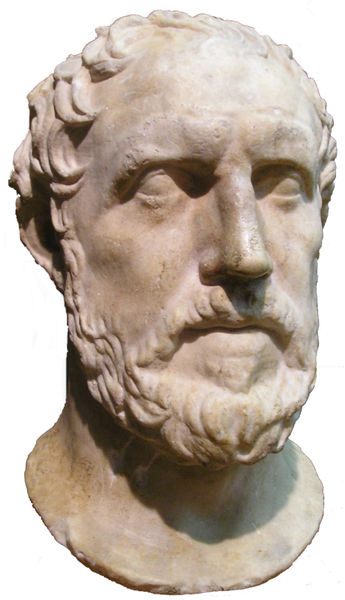
\includegraphics[width=0.9\textwidth]{FIGS/Thucydides-bust-noBG}
\end{center}
\end{minipage}
}

\begin{frame}{How infectious pathogens become mobile}
\bbullet
I used to show the following set of figures to illustrate the spatialisation of spread
\vfill
\bbullet
I tried to get Gemini to do the same but the ``returning home'' part was not working at all
\vfill
\bbullet
So enjoy my fantastic skills instead
\end{frame}

\maxFrameImage{FIGS/diffusion0}
\maxFrameImage{FIGS/diffusion1}
\maxFrameImage{FIGS/diffusion2}
\maxFrameImage{FIGS/diffusion3}
\maxFrameImage{FIGS/diffusion4}
\maxFrameImage{FIGS/diffusion5}
\maxFrameImage{FIGS/diffusion6}
\maxFrameImage{FIGS/diffusion7}
\maxFrameImage{FIGS/diffusion8}

\begin{frame}{So...}
\bbullet Bakery-driven pathogen spread
\vfill
\bbullet Joke aside, let's consider two examples
\end{frame}

\maxFrameImage{FIGS/SARS_CoV_halo}
\maxFrameImage{FIGS/SARS_countries_with_time}

\begin{frame}
\frametitle{Spatial spread of pH1N1 in 2009}
\nocite{KhanArinoHuRaposoEtAl2009}
	In March and April 2008 (used as surrogate for 2009 data), 
	\begin{itemize}
		\item 2.35 million passengers flew from MX to 1018 cities in 164 countries
		\item 80.7\% flew to US and Canada, 8.8\% South and Central America, 8.7\% Europe
		\item of 20 countries with highest volumes of passengers arriving from MX, 16 had confirmed importations from MX on 5/25
		\item ROC curve of relationship between international air-traffic flows
		and H1N1 importation: countries receiving more than 1400 passengers from MX at significantly elevated risk for importation
		\item Use this passenger threshold: international air-traffic volume 
		$>92\%$ sensitive and $>92\%$ specific in predicting importation (area under ROC curve 0.97)
	\end{itemize}
	\vfill
	\begin{flushright}
		Khan, JA, Hu et al, New England Journal of Medicine, 2009
	\end{flushright}
\end{frame}
\maxFrameImage{FIGS/VOC_countries_reporting_since_first_case_2022_04_07}

\maxFrameImage{FIGS/vaccine_coverage_Africa}
\maxFrameImage{FIGS/West_Central_Africa_Polio_2000_2006_noNGA}
\maxFrameImage{FIGS/West_Central_Africa_Polio_2000_2006}
\maxFrameImage{FIGS/spread_polio_from_Nigeria}

\begin{frame}{In a globalised world}
\bbullet
Public health policy decisions are taken at the jurisdictional level, typically national (ISO 3166-1) or first-level sub-national (ISO 3166-2) -- extremely rarely supra-nationally
\vfill
(International Health Regulations (IHR) define processes regarding reporting of disease outbreaks, make recommendations about handling of travellers, etc. See COVID-19: even those of the rules that were somewhat prescriptive were not followed)
\vfill
\bbullet
Individuals are mobile and thus so are the pathogens they harbour
\vfill
\bbullet 
Policy decisions have consequences outside the jurisdictions where they are taken!
\vfill
\bbullet
COVID-19 was a single outbreak, not one outbreak per country it affected
\end{frame}




%%%%%%%%%%%%%%%%%%%
%%%%%%%%%%%%%%%%%%%
%%%%%%%%%%%%%%%%%%%
%%%%%%%%%%%%%%%%%%%
\section{Metapopulations for disease spread modelling}
\newSectionSlide{FIGS-slides-admin/Gemini_Generated_Image_vqpscpvqpscpvqps.jpeg}
%%%%%%%%%%%%%%%%%%%
%%%%%%%%%%%%%%%%%%%
\subsection{Why use metapopulation models?}
\newSubSectionSlide{FIGS-slides-admin/Gemini_Generated_Image_vqpscpvqpscpvqps.jpeg}

\frame {\frametitle{Why use metapopulations for disease models?}
\begin{itemize}
\item Appropriate for the description of spatial spread of some diseases
\vfill
\item Ease of simulation
\vfill
\item Aggregation of data by governments is most often done at the jurisdictional level, very easy to reconcile with locations in metapopulations
\end{itemize}
}

\begin{frame}{A few pointers}
	\begin{itemize}
		\item JA \& PvdD. \href{https://julien-arino.github.io/assets/pdf/papers/2006_ArinoPvdD-FIC48.pdf}{Disease spread in metapopulations}. \emph{Fields Institute Communications} \textbf{48}:1-13 (2006) \nocite{ArinoVdD2006a}
		\vfill
		\item JA. \href{https://julien-arino.github.io/assets/pdf/papers/2009_Arino-metapopulations.pdf}{Diseases in metapopulations}. In \emph{Modeling and Dynamics of Infectious Diseases}, World Scientific (2009) \nocite{Arino2009}
		\vfill
		\item JA. \href{https://doi.org/10.1016/j.idm.2017.05.001}{Spatio-temporal spread of infectious pathogens of humans}. \emph{Infectious Disease Modelling} \textbf{2}(2):218-228 (2017) \nocite{Arino2017}
		\vfill
		\item JA, Bajeux \& Kirkland. \href{https://doi.org/10.1007/s11538-019-00593-1}{Number of source patches required for population persistence in a source-sink metapopulation}. \emph{Bulletin of Mathematical Biology} \textbf{81}: 1916–1942 (2019) \nocite{ArinoBajeuxKirkland2019}
	\end{itemize}
\end{frame}


%%%%%%%%%%%%%%%%%%%
%%%%%%%%%%%%%%%%%%%
\subsection[Explicit movement]{Metapopulations with explicit movement}
\newSubSectionSlide{FIGS-slides-admin/Gemini_Generated_Image_vqpscpvqpscpvqps.jpeg}


\frame{\frametitle{Metapopulations with explicit movement}
	Split continuous space into $N$ discrete geographical locations (\emph{ptatches})
	\vfill
	Each location contains \textbf{compartments} (homogeneous groups of individuals). E.g., preys, predators, etc. 
	\vfill
	Here, we consider a single compartment, the \emph{species of interest}, with no further compartmentalisation
	\vfill
	Individuals \emph{may} move between locations; $m_{qp}\geq 0$ rate of movement of individuals from location $p=1,\ldots,N$ to location $q=1,\ldots,N$
}

\frame{\frametitle{Explicit movement (focus on $P_1$)}
	\begin{center}		
	\begin{tikzpicture}[auto, %node distance = 2cm, auto,
	cloud/.style={minimum width={width("N-1")+2pt},
		draw, ellipse,fill=red!20}]
	\node [cloud] (P1) {$P_1$};
	\node [cloud, above right=of P1] (P2) {$P_2$};
	\node [cloud, right=of P1] (P3) {$P_3$};
	\node [cloud, below right=of P1] (P4) {$P_4$};
	\node [cloud, below=of P1] (P5) {$P_5$};
	\node [cloud, below left=of P1] (P6) {$P_6$};
	\node [cloud, above left=of P1] (Pk) {$P_k$};
	%% Outflows
	\path [line, very thick, blue] (P1) to [bend left = 20] node [midway, left] (TextNode) {$m_{21}$} (P2);
	\path [line, very thick, blue] (P1) to [bend left = 20] node [midway, below] (TextNode) {$m_{31}$} (P3);
	\path [line, very thick, blue] (P1) to [bend left = 20] node [pos=0.9, right] (TextNode) {$m_{51}$} (P5);
	\path [line, very thick, blue] (P1) to [bend left = 20] node [midway, right] (TextNode) {$m_{61}$} (P6);
	\path [line, very thick, blue, densely dashed] (P1) to [bend left = 20] node [midway, left] (TextNode) {$m_{k1}$} (Pk);
	%% Inflows
	\path [line, very thick, red] (P2) to [bend left = 20] node [midway, right] (TextNode) {$m_{12}$} (P1);
	\path [line, very thick, red] (P4) to [bend left = 20] node [right] (TextNode) {$m_{14}$} (P1);
	\path [line, very thick, red] (P6) to [bend left = 20] node [left] (TextNode) {$m_{16}$} (P1);
	\path [line, very thick, red, densely dashed] (Pk) to [bend left = 20] node [right, pos=0.1] (TextNode) {$m_{1k}$} (P1);
	\end{tikzpicture}
	\end{center}
	\[
	P_1' = {\red \sum_{\substack{j=1\\j\neq 1}}^{N}m_{1j}P_j}
	{\blue -P_1\sum_{\substack{j=1\\j\neq 1}}^{N}m_{j1}}
	\]
	or
	\[
	P_1' = \sum_{j=1}^{N} m_{1j}P_j
	\textrm{ assuming }
	m_{11}=-\sum_{\substack{j=1\\j\neq 1}}^{N} m_{j1}
	\]
}



%%%%%%%%%%%%%%%%%%%
%%%%%%%%%%%%%%%%%%%
\subsection{The graph setting}
\newSubSectionSlide{FIGS-slides-admin/Gemini_Generated_Image_vqpscpvqpscpvqps.jpeg}


\begin{frame}\frametitle{Graph setting}
Suppose
\begin{itemize} 
\item $|\P|$ locations, vertices in a (directed) graph $\G$
\item Each location contains a certain number of compartments belonging to a common set $\C$ of compartments
\item Arcs of $\G$ represent the possibility for a given compartment to move between two locations; any two locations are connected by a maximum of $|\C|$ edges
\end{itemize}
\vfill
Graph is a digraph: movement is not always symmetric
\end{frame}


\begin{frame}
$\G=(\P,\A)$ is multi-digraph, where 
\begin{itemize}
	\item $\P$ is the set of vertices (locations)
	\item $\A$ is the set of arcs, i.e., an ordered multiset of pairs of elements of $\P$
\end{itemize}
\vfill
Any two vertices $X,Y\in\P$ are connected by at most $|\C|$ arcs from $X$ to $Y$ and at most $|\C|$ arcs from $Y$ to $X$
\vfill
Because there are $|\C|$ compartments and movements are compartment-specific, we also define, for all $c\in\C$, $\P_c$ and $\A_c$ as well as the compartment-specific digraphs $\G^c=(\P_c,\A_c)$
\end{frame}



\frame{\frametitle{Connection matrix}
For a given compartment $c\in\C$, a \emph{connection matrix} can be associated to the digraph $\G_c$
\vfill
This is the \textbf{adjacency matrix} of $\G_c$, but we emphasize the reason why we use $\G_c$ by using the term \emph{connection}
\vfill
Choosing an ordering of elements of $\P$, the $(i,j)$ entry of the $|\P|\times|\P|$-matrix $\N_c=\N_c(\G_c)$ is one if $R^c(P_i,P_j)$ and zero otherwise, i.e., if $P_i$ has no direct access to $P_j$
\vfill
For convenience, the ordering of the locations is generally assumed the same for all compartments
}


\frame{\frametitle{Srong connectedness and irreducibility}
\begin{definition}[Reducible/irreducible matrix]
	\label{def:reducible_irreducible_matrix}
	A matrix $A$ is \textbf{reducible} if there exists a permutation matrix $P$ such that $P^TAP$ is block upper triangular. A matrix that is not reducible is \textbf{irreducible}
\end{definition}
\vfill
Matrix $A\in\IF^{n\times n}$ is irreducible if for all $i,j=1,\ldots,n$, there exists $k$ such that $a_{ij}^k>0$, where $a_{ij}^k$ is the $(i,j)$-entry in $A^k$
\vfill
\begin{theorem}
	Strong connectedness $\Leftrightarrow$ \textbf{irreducibility} of the connection matrix $\mathcal{C}_c$
\end{theorem}
}


%%%%%%%%%%%%%%%%%%%
%%%%%%%%%%%%%%%%%%%
\subsection{The models considered}
\newSubSectionSlide{FIGS-slides-admin/Gemini_Generated_Image_vqpscpvqpscpvqps.jpeg}


\frame{\frametitle{The prototype SLIRS used in patches}
\begin{center}
	\begin{tikzpicture}[scale=1, every node/.style={transform shape},
		auto, %node distance = 2cm, auto,
		box/.style={minimum width={width("N-1")+2pt},
			draw, rectangle,fill=gray!20}]
		%% States
		\node [box] at (0,2) (S) {$S$};
		\node [box] at (2,2) (L) {$L$};
		\node [box] at (4,2) (I) {$I$};
		\node [box] at (6,2) (R) {$R$};
		%% Flows
		\path [line, thick] (-1.25,2) to node [midway, above] (TextNode) {$b$} (S);
		\path [line, thick] (S) to node [midway, above, sloped] (TextNode) {$\Phi$} (L);
		\path [line, thick] (L) to node [midway, above] (TextNode) {$\varepsilon L$} (I);
		\path [line, thick] (I) to node [sloped, midway, above] (TextNode) {$\gamma I$} (R);
		\draw [>=latex,->, thick, rounded corners] (R) -- +(0,0.75) -- ++(-6,0.75) node[midway, above] {$\nu R$} -- (S);
		\path [line, thick] (S) to node [midway, right] (TextNode) {$dS$} ++(0,-1);
		\path [line, thick] (L) to node [midway, right] (TextNode) {$dL$} ++(0,-1);
		\path [line, thick] (I) to node [midway, right] (TextNode) {$dI$} ++(0,-1);
		\path [line, thick] (R) to node [midway, right] (TextNode) {$dR$} ++(0,-1);
	\end{tikzpicture}
\end{center}
\begin{subequations}\label{sys:SLIRS}
\begin{align}
S' &= b+\nu R-\Phi-dS \\
L' &= \Phi-(\varepsilon+d)L\\
I' &= \varepsilon L-(\gamma+d)I\\
R' &= \gamma I-(\nu+d)R
\end{align}
\end{subequations}
$\Phi$ force of infection. Depends on $S,I$, possibly $N$. In general
\[
\Phi=\beta(N)\phi(S,I)
\] 

Mass action, $\Phi=\beta SI$, proportional incidence, $\Phi=\beta SI/N$
}



\frame{\frametitle{$|\mathcal{P}|$-SLIRS model}
\begin{subequations}
	\label{sys:pSLIRS}
	\begin{align}
		S_{p}' &=b_p+\nu_pR_p-\Phi_p-d_pS_p 
		\color{red}{+\textstyle{\sum_{q\in\mathcal{P}}} m_{Spq}S_{q}} 
		\label{sys:pSLIRS_dS} \\
		L_{p}' &=\Phi_p-\left( \varepsilon_{p}+d_{p}\right)L_{p}
		\color{red}{+\textstyle{\sum_{q\in\mathcal{P}}} m_{Lpq}L_{q}} 
		\label{sys:pSLIRS_dL} \\
		I_{p}' &=\varepsilon_pL_p-(\gamma_p+d_p)I_p
		\color{red}{+\textstyle{\sum_{q\in\mathcal{P}}} m_{Ipq}I_{q}} 
		\label{sys:pSLIRS_dI} \\
		R_{p}' &=\gamma _{p}I_{p}-\left(\nu_{p}+d_{p}\right)R_{p}
		\color{red}{+\textstyle{\sum_{q\in\mathcal{P}}} m_{Rpq}R_{q}} 
		\label{sys:pSLIRS_dR} 
	\end{align}
	with incidence 
	\begin{equation}
		\Phi_p=\beta_p\frac{S_pI_p}{N_p^{q_p}},\qquad q_p\in\{0,1\}
		\label{sys:pSLIRS_incidence} 
	\end{equation}
\end{subequations}	
}

\begin{frame}
\frametitle{$|\S|\;|\P|$-SLIRS (multiple species)}
$p\in\P$ and $s\in\mathcal{S}$ (a set of species)
\vfill
\begin{subequations}
	\label{sys:spSLIRS}
	\begin{align}
		S_{sp}' &= b_p+\nu_{sp}R_{sp}-\Phi_{sp}-d_{sp}S_{sp}
		\color{red}{+\textstyle{\sum_{q\in\mathcal{P}}} m_{Sspq}S_{sq}} 
		\label{sys:spSLIRS_dS} \\
		L_{sp}' &= \Phi_{sp}-(\varepsilon_{sp}+d_{sp})L_{sp}
		\color{red}{+\textstyle{\sum_{q\in\mathcal{P}}}m_{Lspq}L_{sq}}
		\label{sys:spSLIRS_dL} \\
		I_{sp}' &= \varepsilon_{sp}L_{sp}-(\gamma_{sp}+d_{sp})I_{sp}
		\color{red}{+\textstyle{\sum_{q\in\mathcal{P}}} m_{Ispq}I_{sq}}
		\label{sys:spSLIRS_dI} \\
		R_{sp} &= \gamma _{sp}I_{sp}-(\nu_{sp}+d_{sp})R_{sp}
		\color{red}{+\textstyle{\sum_{q\in\mathcal{P}}} m_{Rspq}R_{sq}} 
		\label{sys:spSLIRS_dR} 
	\end{align}
	with incidence
	\begin{equation}
	\Phi_{sp}=\sum_{k\in\mathcal{S}}\beta_{skp}\frac{S_{sp}I_{kp}}{N_p^{q_p}},\qquad q_p\in\{0,1\}
	\label{sys:spSLIRS_incidence} 
	\end{equation}
\end{subequations}
\vfill
{\tiny
\begin{itemize}
\setlength{\itemsep}{-5pt}
\item JA, Davis, Hartley, Jordan, Miller \& PvdD. \href{https://julien-arino.github.io/assets/pdf/papers/2005_ArinoDavisHartleyJordanMillerPvdD-MMB22.pdf}{A multi-species epidemic model with spatial dynamics}. \emph{Mathematical Medicine and Biology} \textbf{22}(2):129-142 (2005) \nocite{ArinoDavisHartleyJordanEtAl2005}
\newline 
\item JA, Jordan \& PvdD. \href{https://julien-arino.github.io/assets/pdf/papers/2007_ArinoJordanPvdD-MBS206.pdf}{Quarantine in a multi-species epidemic model with spatial dynamics}. \emph{Mathematical Biosciences} \textbf{206}(1):46-60 (2007) \cite{ArinoJordanPvdD2007}
\end{itemize}}
\end{frame}

\frame{
\frametitle{$|\P|^2$-SLIRS (residents-travellers)}
\begin{subequations}
	\label{sys:ppSLIRS}
	\begin{align}
		S_{pq}' =& 
		b_p+\nu_{pq} R_{pq}-\Phi_{pq}-d_{pq}S_{pq} \color{red}{+\textstyle{\sum_{k\in\mathcal{P}}} m_{Spqk}S_{pk}} 
		\label{sys:ppSLIRS_dS} \\
		L_{pq}' =& \Phi_{pq}
		-(\varepsilon_{pq}+d_{pq})L_{pq}
		\color{red}{+\textstyle{\sum_{k\in\mathcal{P}}} m_{Lpqk}L_{pk}} 
		\label{sys:ppSLIRS_dL} \\
		I_{pq}' =& \varepsilon_{pq} L_{pq}
		-(\gamma_{pq}+d_{pq})I_{pq}
		\color{red}{+\textstyle{\sum_{k\in\mathcal{P}}} m_{Ipqk}I_{pk}} 
		\label{sys:ppSLIRS_dI} \\
		R_{pq}' =& \gamma_{pq} I_{pq}
		-(\nu_{pq}+d_{pq})R_{pq}
		\color{red}{+\textstyle{\sum_{k\in\mathcal{P}}} m_{Rpqk}R_{pk}}
		\label{sys:ppSLIRS_dR} 
	\end{align}
	with incidence
	\begin{equation}
		\Phi_{pq}=\sum_{k\in\mathcal{P}}\beta_{pqk}\frac{S_{pq}I_{kq}}{N_p^{q_q}},\qquad q_q=\{0,1\}
		\label{sys:ppSLIRS_incidence} 
	\end{equation}
\end{subequations}

\vfill
{\tiny
\begin{itemize}
%\setlength{\itemsep}{-5pt}
\item Sattenspiel \& Dietz. \href{https://doi.org/10.1016/0025-5564(94)00068-B}{A structured epidemic model incorporating geographic mobility among regions} (1995) \nocite{sattenspiel1995structured}
\item JA \& PvdD. \href{https://julien-arino.github.io/assets/pdf/papers/2003_ArinoPvdD-MPS10_correct.pdf}{A multi-city epidemic model}. \emph{Mathematical Population Studies} \textbf{10}(3):175-193 (2003) \nocite{ArinoVdD2003a}
\item JA \& PvdD. \href{https://julien-arino.github.io/assets/pdf/papers/2003_ArinoPvdD-LNCIS294.pdf}{The basic reproduction number in a multi-city compartmental epidemic model}. In \emph{Positive Systems} (2003) \nocite{ArinoVdD2003b}
\end{itemize}}
}


\frame{\frametitle{Steps for an analysis}
\textbf{Basic steps}
\begin{enumerate}
\item Well-posedness of the system
\item Existence of disease free equilibria (DFE)
\item Computation of a reproduction number $\R_0$, study local asymptotic stability of DFE
\item If DFE unique, prove global asymptotic stability when $\R_0<1$
\end{enumerate}
\textbf{Additional steps}
\begin{enumerate}\setcounter{enumi}{4}
\item Existence of \emph{mixed} equilibria, with some locations at DFE and others with disease
\item Computation of some bounds on $\R_0$
\item EEP and its LAS \& GAS properties
\end{enumerate}
$\ldots$
}

\begin{frame}{Analysis -- Toy system}
For simplicity, consider $|\mathcal{P}|$-SLIRS with $\mathcal{B}_p(N_p)=b_p$
\begin{subequations}
	\label{sys:pSLIRS_toy}
	\begin{align}
		S_{p}' &=b_p-\Phi_p-d_pS_p+\nu_pR_p
		+\textstyle{\sum_{q\in\mathcal{P}}} m_{Spq}S_{q} 
		\label{sys:pSLIRS_toy_dS} \\
		L_{p}' &=\Phi_p-\left( \varepsilon_{p}+d_{p}\right)L_{p}
		+\textstyle{\sum_{q\in\mathcal{P}}} m_{Lpq}L_{q} 
		\label{sys:pSLIRS_toy_dL} \\
		I_{p}' &=\varepsilon_pL_p-(\gamma_p+d_p)I_p
		+\textstyle{\sum_{q\in\mathcal{P}}} m_{Ipq}I_{q} 
		\label{sys:pSLIRS_toy_dI} \\
		R_{p}' &=\gamma _{p}I_{p}-\left(\nu_{p}+d_{p}\right)R_{p}
		+\textstyle{\sum_{q\in\mathcal{P}}} m_{Rpq}R_{q}
		\label{sys:pSLIRS_toy_dR} 
	\end{align}
	with incidence
	\begin{equation}
		\Phi_p=\beta_pS_pI_p
		\label{sys:pSLIRS_toy_incidence} 
	\end{equation}			
\end{subequations}
\vfill
System of $4|\mathcal{P}|$ equations
\end{frame}

\begin{frame}{Don't panic: size is not that bad..}
System of $4|\mathcal{P}|$ equations !!!
\vfill
However, a lot of structure: 
\begin{itemize}
	\item $|\mathcal{P}|$ \emph{copies} of individual units, each comprising 4 equations
	\item Dynamics of individual units well understood
	\item Coupling is linear
\end{itemize}
\vfill
$\implies$ Good case of large-scale system
\vfill
(matrix analysis is your friend)

\end{frame}




%%%%%%%%%%%%%%%%%%%
%%%%%%%%%%%%%%%%%%%
\subsection{Going to vector form}
\newSubSectionSlide{FIGS-slides-admin/Gemini_Generated_Image_vqpscpvqpscpvqps.jpeg}

\frame{\frametitle{Notation}
\begin{itemize}
	\item $X_{cp}(t)$ number of individuals of compartment $c$ in location $p$ at time $t$
	\vfill
	(Here and elsewhere: omit dependence on $t$ unless it causes confusion)
	\vfill
	\item $\bX_c=\left(X_{c1},\ldots,X_{c|\P|}\right)^T$ distribution of individuals of compartment $c\in\C$ among the different locations 
	\newline
	[E.g., for \eqref{sys:pSLIRS_toy}, $\bX_S=(S_1,\ldots,S_{|\P|})^T$]
	\vfill
	\item $\bX^p=\left(X_1^p,\ldots,X_{|\P|}^p\right)^T$ composition of the population in location $p\in\P$
	\newline
	[E.g., for \eqref{sys:pSLIRS_toy}, $\bX^p=(S_p,L_p,I_p,R_p)^T$]
\end{itemize}
}

\frame{\frametitle{Metapopulation models with linear movement}
Use a linear autonomous movement operator
\vfill
Then, for a given compartment $c\in\C$ and in a given location $p\in\P$
\[
	X_{cp}'=f_{cp}(\bX^p)
	+\sum\dind{q\in\P}{q\neq p}m_{cpq}X_{cq} 
	-\left(\sum\dind{q\in\P}{q\neq p}m_{cqp}\right)X_{cp}
\]
where $m_{cpq}$ rate of movement of individuals in compartment $c\in\C$ from location $q\in\P$ to location $p\in\P$
}

\begin{frame}{A more compact notation}
	To make 
	\[
		X_{cp}'=f_{cp}(\bX^p)
		+\sum\dind{q\in\P}{q\neq p}m_{cpq}X_{cq} 
		-\left(\sum\dind{q\in\P}{q\neq p}m_{cqp}\right)X_{cp}
	\]
	more compact, denote the rate of leaving location $p$ as
	\begin{equation}
		m_{cpp} = -\sum\dind{q\in\P}{q\neq p}m_{cqp}
	\end{equation}
	Then
	\begin{equation}\label{eq:general_metapop_linear_migration}
		X_{cp}'=f_{cp}(\bX^p)+\sum_{q\in\P}m_{cpq}X_{cq}
	\end{equation}
\end{frame}

\begin{frame}{Vector form of the system}
For compartment $c\in\C$,
\begin{equation}\label{eq:general_metapop}
\bX_c'=f(\bX)+\mathcal{M}_c\bX_c
\end{equation}
with
\begin{equation}\label{eq:movement_matrix}
\mathcal{M}_c =
\begin{pmatrix}
-\sum\limits_{k\in\P}m_{ck1} & m_{c12} & \cdots & m_{c1|\P|} \\
& & & \\
m_{c|\P|1} & m_{c|\P|2} & \cdots & -\sum\limits_{k\in\P}m_{ck|\P|}
\end{pmatrix}
\end{equation}
\end{frame}


%%%%%%%%%%%%%%%%%%
%%%%%%%%%%%%%%%%%%
\subsection{The movement matrix}
\newSubSectionSlide{FIGS-slides-admin/Gemini_Generated_Image_ebceq5ebceq5ebce.jpeg}

\begin{frame}{Definitions and notation for matrices}
\begin{itemize}
	\item $M\in\mathbb{R}^{n\times n}$ a square matrix with entries denoted $m_{ij}$
	\vfill
	\item $M\geq\mathbf{0}$ if $m_{ij}\geq 0$ for all $i,j$ (could be the zero matrix); $M>\mathbf{0}$ if $M\geq\mathbf{0}$ and $\exists i,j$ with $m_{ij}>0$; $M\gg\mathbf{0}$ if $m_{ij}>0$ $\forall i,j=1,\ldots,n$. Same notation for vectors
	\vfill
	\item $\sigma(M)=\{\lambda\in\mathbf{C}; M\lambda=\lambda\mathbf{v}, \mathbf{v}\neq\mathbf{0}\}$ \textbf{spectrum} of $M$
	\vfill
	\item $\rho(M)=\max_{\lambda\in\sigma(M)}\{|\lambda|\}$ \textbf{spectral radius}
	\vfill
	\item $s(M)=\max_{\lambda\in\sigma(M)}\{\Re(\lambda)\}$ \textbf{spectral abscissa} (or \textbf{stability modulus})
	\vfill
	\item $M$ is an \textbf{M-matrix} if it is a \textbf{Z-matrix} ($m_{ij}\leq 0$ for $i\neq j$) and $M = s\mathbb{I}-A$, with $A\geq 0$ and $s\geq \rho(A)$
\end{itemize}
\end{frame}

\begin{frame}{The movement matrix}
	The matrix
	\begin{equation}\tag{\ref{eq:movement_matrix}}
		\mathcal{M}_c =
		\begin{pmatrix}
		-\sum\limits_{k\in\P}m_{ck1} & m_{c12} & \cdots & m_{c1|\P|} \\
		& & & \\
		m_{c|\P|1} & m_{c|\P|2} & \cdots & -\sum\limits_{k\in\P}m_{ck|\P|}
		\end{pmatrix}
	\end{equation}
	is the \textbf{movement matrix}
	\vfill
	It plays an extremely important role in the analysis of metapopulation systems, so we'll spend some time discussing its properties
	\vfill
$\mathcal{M}_c$ describes
\begin{itemize} 
\item existence of connections
\item when they exist, their ``intensity''
\end{itemize}
\end{frame}

\begin{frame}{Properties of the movement matrix $\M$}
	First, remark $-\M_c$ is a weighted Laplacian matrix (using out-degrees)
	\vfill
	\begin{lemma}\label{lemma:behaviour_Mc}
		\begin{enumerate}
			\item $0\in\sigma(\M)$ corresponding to left e.v. $\11^T$ \hfill[$\sigma$ spectrum]
			\item $-\M$ is a singular M-matrix
			\item $0=s(\M)\in\sigma(\M)$ \hfill[$s$ spectral abscissa]
			\item If $\M$ irreducible, then $s(\M)$ has multiplicity 1
		\end{enumerate}
	\end{lemma}
	\vfill
	For complete proof of Lemma~\ref{lemma:behaviour_Mc} and Proposition~\ref{prop:behaviour_Mc} (next page), see \href{http://dx.doi.org/10.1007/s11538-019-00593-1}{Arino, Bajeux \& Kirkland, BMB 2019}
\end{frame}

\begin{frame}
	\begin{proposition}[$D$ a diagonal matrix]
		\label{prop:behaviour_Mc}
		\begin{enumerate}
			\item $s(\M+d\II)=d$, $\forall d\in\IR$
			\item $s(\M+D)\in\sigma(\M+D)$ associated to $\bv>\b0$. If $\M$ irreducible, $s(\M+D)$ has  multiplicity 1 and is associated to $\bv\gg \b0$
			\item If $\diag (D)\gg \b0$, then $D-\M$ invertible M-matrix and $(D-\M)^{-1}> \b0$
			\item $\M$ irreducible and $\diag(D)>\b0$ $\Longrightarrow$ $D-\M$ nonsingular irreducible M-matrix and $(D-\M)^{-1}\gg \b0$		
		\end{enumerate}
	\end{proposition}
\end{frame}


%%%%%%%%%%%%%%%%%
%%%%%%%%%%%%%%%%%
\subsection{Behaviour of the mobility component}
\newSubSectionSlide{FIGS-slides-admin/Gemini_Generated_Image_vqpscpvqpscpvqps.jpeg}


\frame{\frametitle{Behaviour of the mobility component -- No demography}
Assume no within-location dynamics, just movement. Then \eqref{eq:general_metapop} takes the form
\begin{equation}\label{eq:mobility_compartment}
	\bX_c' = \mathcal{M}_c\bX_c
\end{equation}
\vfill
\begin{theorem}\label{th:GAS_metapop1}
For a given compartment $c\in\C$, suppose that the movement matrix $\M_c$ is irreducible. Then for any $\bX_c(0)>0$, \eqref{eq:mobility_compartment} satisfies
\[
\lim_{t\to\infty}\bX_c(t)=\bX_c^\star\gg 0
\]
\end{theorem}
\vfill
Note that $\bX_c^\star$ depends on $\langle\nbOne,\bX_c(0)\rangle$
}


\begin{frame}{Reduction to total population per location -- Demography}
Let 
\[
	T_p = \sum_{c\in\C}X_{cp}
\]
be the total population in location $p$
\vfill
It is often posssible to obtain, in each location $p\in\P$, an equation for the evolution of the total population that takes the form
\begin{equation}\label{eq:dT_total_population}
	T_p' = 
	D_p(T_p)+\sum_{c\in\C}\sum_{q\in\P}m_{cpq}X_{cq}
\end{equation}
where $D_p(T_p)$ describes the demography in location $p$
\end{frame}

\begin{frame}{Nature of the demography}
	Most common types of demographic functions
	\begin{itemize}
		\item $D_p(T_p)=b_p-d_pT_p$ (asymptotically constant population)
		\item $D_p(T_p)=b_pT_p-d_pT_p$ 
		\item $D_p(T_p)=d_pT_p-d_pT_p=0$ (constant population)
		\item $D_p(T_p)=r_pT_p(1-T_p/K_p)$ (logistic demography)
	\end{itemize}
	\vfill
	We have assumed (since birth term is $b_p$) 
	\begin{equation}\label{eq:demography_function}
		D_p(T_p)=b_p-d_pT_p
	\end{equation}
\end{frame}

\begin{frame}{Vector / matrix form of the equation}
Assuming demography is of the form \eqref{eq:demography_function}, write \eqref{eq:dT_total_population} in vector form
\begin{equation}\label{sys:dN_general} 
	\mathbf{T}'=\mathbf{b}-\bd\bT+\sum_{c\in\C}\mathcal{M}_c\bX_{c}	
\end{equation}
where 
\begin{itemize}
	\item $\mathbf{b}=(b_1,\ldots,b_{|\mathcal{P}|})^T\in\IR^{|\P|}$
	\item $\mathbf{T}=(T_1,\ldots,T_{|\mathcal{P}|})^T\in\IR^{|\P|}$
	\item $\mathbf{X}=(X_{c1},\ldots,X_{c{|\mathcal{P}|}})^T\in\IR^{|\P|}$
	\item $\bd=\mathsf{diag}\left(d_1,\ldots,d_{|\mathcal{P}|}\right)\in\IR^{|\mathcal{P}|\times|\mathcal{P}|}$
	\item $\mathcal{M}_c\in\IR^{|\mathcal{P}|\times|\mathcal{P}|}$
\end{itemize}

\end{frame}


\begin{frame}{The nice case}
Suppose movement rates \textbf{equal for all compartments}, i.e.,
$$
\M_c\equiv\M
$$
\vfill
(stronger than the property of movement being \emph{similar for all compartments}, which only requires zero/nonzero patterns in all $\M_c$, $c\in\C$, to be the same)
\vfill
Then
\begin{align}
\bT' &= \bb-\bd\bT+\M\sum_{c\in\C}\bN_{c} \nonumber \\
&= \bb-\bd\bT+\M\bT \label{sys:pSLIRS_toy_dN}
\end{align}
\end{frame}


\begin{frame}{Equilibria}
$$
\begin{aligned}
\bT'=\b0 &\Leftrightarrow \mathbf{b}-\bd\mathbf{T}+\mathcal{M}\mathbf{T}=\mathbf{0} \\
&\Leftrightarrow (\bd-\mathcal{M})\mathbf{T}=\mathbf{b} \\
&\Leftrightarrow \mathbf{T}^\star=(\bd-\mathcal{M})^{-1}\mathbf{b}
\end{aligned}
$$
given, of course, that $\bd-\mathcal{M}$ (or, equivalently, $\mathcal{M}-\bd$) is invertible.. 
\vfill
Is it?
\end{frame}

\begin{frame}{Nonsingularity of $\mathcal{M}-\bd$}
Using the spectrum shift of Theorem~\ref{prop:behaviour_Mc}{(1)}
\[
s\left(\mathcal{M}-\min_{p\in\mathcal{P}}d_p\right)=-\min_{p\in\mathcal{P}}d_p
\]
This gives a constraint: for total population to behave well (in general, we want this), we \emph{must assume all death rates are positive}
\vfill
Assume they are (in other words, assume $\bd$ nonsingular). Then $\mathcal{M}-\bd$ is nonsingular and $\bT^\star=(\bd-\mathcal{M})^{-1}\mathbf{b}$ unique
\end{frame}


\begin{frame}{Behaviour of the total population}
\framesubtitle{Equal irreducible movement case}
$\mathbf{T}^\star=(\bd-\mathcal{M})^{-1}\mathbf{b}$ attracts solutions of
$$
\mathbf{T}'=\mathbf{b}-\bd\mathbf{T}+\mathcal{M}\mathbf{T}=:f(\mathbf{T})
$$
\vfill
Indeed, we have
$$
Df=\mathcal{M}-\bd
$$
\vfill
Since we now assume that $\bd$ is nonsingular, we have by Theorem~\ref{prop:behaviour_Mc}{(1)} that $s(\mathcal{M}-\min_{p\in\mathcal{P}}d_p)=-\min_{p\in\mathcal{P}}d_p<0$
\vfill
$\mathcal{M}$ irreducible $\rightarrow$ $\mathbf{T}^\star\gg 0$ (provided $\mathbf{b}>\mathbf{0}$, of course)
\end{frame}


\begin{frame}{Behaviour of total population (equal \emph{reducible} movement)}
\begin{theorem}
Assume $\mathcal{M}$ reducible. Let $a$ be the number of minimal absorbing sets in the corresponding connection graph $\mathcal{G}(\mathcal{M})$. Then
\begin{enumerate}
	\item The spectral abscissa $s(\mathcal{M})=0$ has multiplicity $a$
	\item Associated to $s(\mathcal{M})$ is a nonnegative eigenvector $\mathbf{v}$ s.t.
	\begin{itemize}
		\item $v_i>0$ if $i$ is a vertex in a minimal absorbing set
		\item $v_i=0$ if $i$ is a transient vertex
	\end{itemize}
\end{enumerate}
\end{theorem}

\vfill
From Foster and Jacquez, \href{https://doi.org/10.1016/0025-5564(75)90096-6}{Multiple zeros for eigenvalues and the multiplicity of traps of a linear compartmental system}, \emph{Mathematical Biosciences} (1975) \nocite{foster1975multiple}
\end{frame}


\begin{frame}{The not-so-nice case}
Recall that
$$
\bT'=\mathbf{b}-\bd\bT+\sum_{c\in\C}\mathcal{M}_c\bX_{c}
$$

Suppose movement rates \textbf{similar for all compartments}, i.e., the zero/nonzero patterns in all matrices are the same but not the entries

Let
$$
\underline{\mathcal{M}}=\left[\min_{c\in\C}m_{cpq}\right]_{pq,p\neq q}\qquad 
\underline{\mathcal{M}}=\left[\max_{c\in\C}m_{cpq}\right]_{pq,p=q}
$$
and
$$
\overline{\mathcal{M}}=\left[\max_{c\in\C}m_{cpq}\right]_{pq,p\neq q}\qquad
\overline{\mathcal{M}}=\left[\min_{c\in\C}m_{cpq}\right]_{pq,p=q}
$$
\end{frame}


\begin{frame}{Cool, no? No!}
Then we have
$$
\mathbf{b}-\bd\mathbf{T}+\underline{\mathcal{M}}\mathbf{T}\leq\mathbf{T}'\leq\mathbf{b}-\bd\mathbf{T}+\overline{\mathcal{M}}\mathbf{T}
$$
\vfill
Me, roughly every 6 months: \emph{Oooh, coooool, a linear differential inclusion!}
\vfill
Me, roughly 10 minutes after making that previous statement: \emph{Quel con!} 
\vfill
Indeed $\underline{\mathcal{M}}$ and $\overline{\mathcal{M}}$ are \textbf{are not} movement matrices  (in particular, their column sums are not all zero)
\vfill
So no luck there.. 
\vfill
We can still do stuff, however more on a case-by-case basis
\end{frame}



% \frame{\frametitle{Boundedness of solutions -- Identical movement rates for all epidemiological states}
% Consider system \eqref{sys:pSEIRS}. Assume $\delta_i=0$ and $M^{S}=M^{E}=M^{I}=M^{R}=:M=[m_{ij}]$. 
% Total population $N_i$ in location $i$:
% \begin{equation}\label{eq:N_pSEIRS}
% \frac{d}{dt}N_i=\B_i(N_i)-d_iN_i-\delta_i I_i+\sum_{j=1}^{|\P|}m_{ij}N_j -\sum_{j=1}^{|\P|}m_{ji}N_i.
% \end{equation}
% Total population in all locations $\nbOne^TN=N_{1}+N_{2}+\ldots +N_{|\P|}$:
% \begin{equation}
% \dfrac{d}{dt}\nbOne^TN=\dsum\limits_{i=1}^{|\P|}(\B_{i}\left( N_{i}\right)-d_{i}N_{i} 
% -\delta_{i}I_{i}).  \label{eq:dNdt}
% \end{equation}
% If $\B_i(N_i)$ has ``good" properties, $\nbOne^TN(t)$ is bounded.
% }

% \frame{
% \begin{theorem}\label{th:behaviorN_nSEIRS}
% Suppose that in system \eqref{sys:pSEIRS}, movement is identical for all epidemiological states, that the disease is not lethal ($\delta_i=0$), and that in each location, birth compensates natural death, that is, $\B_i(N_i)=d_iN_i$. Then for every location $i=1,\ldots,|\P|$, there holds
% \[
% \lim_{t\to\infty}N_i(t)=N_i^*>0.
% \]
% \end{theorem}
% }

% \frame{\frametitle{Proof}
% Under theorem assumptions, system is linear and decouples from the epidemic variables. For $i=1,\ldots,|\P|$,
% \[
% \dfrac{d}{dt}N_{i}=\dsum\limits_{j=1}^{|\P|}m_{ij}N_{j}-\dsum\limits_{j=1}^{|\P|}m_{ji}^{{}}N_{i}  
% \]
% or
% \[
% \frac{d}{dt}
% \begin{pmatrix}
% N_1 \\
% N_2 \\
% \vdots \\
% N_{|\P|}
% \end{pmatrix}=
% \begin{pmatrix}
% -\sum_{j=1}^{|\P|}m_{j1} & m_{12} & m_{13} & \cdots & m_{1|\P|} \\
% m_{21} & -\sum_{j=1}^{|\P|}m_{j1} & m_{23} & \cdots & m_{2|\P|} \\
% \vdots &\vdots &\vdots& & \vdots \\
% m_{|\P|1} & m_{|\P|2} & m_{|\P|3} & \cdots 
% & -\sum_{j=1}^{|\P|}m_{j|\P|}
% \end{pmatrix}
% \begin{pmatrix}
% N_1 \\
% N_2 \\
% \vdots \\
% N_{|\P|}
% \end{pmatrix}.
% \]
% The result then follows from Theorem~\ref{th:GAS_metapop1}.
% }

% \frame{
% \begin{theorem}\label{th:behaviorN_spSEIRS}
% Suppose that, in system \eqref{sys:spSEIRS}, movement is identical for all epidemiological states, that the disease is not lethal ($\delta_{sp}=0$), and that in each location, birth compensates natural death, that is, $\B_{sp}(N_{sp})=d_{sp}N_{sp}$. Then the movement model is given, for all $s=1,\ldots,|\C|$ and all $p=1,\ldots,|\P|$, by
% \begin{equation}\label{eq:Nsp_spSEIRS}
% \frac{d}{dt}N_{sp}=\sum_{q=1}^{|\P|}m_{spq}N_{sq}-\sum_{q=1}^{|\P|}m_{sqp}N_{sp},
% \end{equation}
% and there holds
% \[
% \lim_{t\to\infty}N_{sp}(t)=N_{sp}^*>0.
% \]
% \end{theorem}
% }

% \frame{
% \begin{theorem}\label{th:behaviorN_ppSEIRS}
% Suppose that, in system \eqref{sys:ppSEIRS}, movement is identical for all epidemiological states, that the disease is not lethal ($\delta_{sp}=0$), and that in each location, birth compensates natural death, that is, 
% \[
% \B_{ij}(N_i^r)=\left\{
% \begin{array}{ll}
% d_{ij}\sum_{k=1}^{|\P|}N_{ik} & \textrm{if } i=j, \\
% 0 & \textrm{if } i\neq j.
% \end{array}
% \right.
% \] 
% Then for every location $i,j=1,\ldots,|\P|$, there holds
% \[
% \lim_{t\to\infty}N_{ij}(t)=N_{ij}^*>0.
% \]
% \end{theorem}
% }

% \frame{
% In the case of system \eqref{sys:ppSEIRS}, boundedness can be obtained with more general birth functions.
% The variation of the number $N_i^r$ of residents in location $i$ is
% given by
% \begin{eqnarray}
% \frac{d}{dt}N^r_i&=& \frac{d}{dt}\sum_{j=1}^{|\P|} N_{ij}
% = \frac{d}{dt}N_{ii}+ \sum\dind{j=1}{j\neq i}^{|\P|}
% \frac{d}{dt}N_{ij} \nonumber\\
% &=& \B_{ii}(N_i^r)+\sum_{k=1}^{|\P|} m_{iik}N_{ik}
% -(d+\sum_{k=1}^n m_{iki})N_{ii} \nonumber \\
% &&+\sum\dind{j=1}{j\neq i}^{|\P|}\left[ \sum_{k=1}^{|\P|} m_{ijk}N_{ik}
% -(d_i+\sum_{k=1}^{|\P|} m_{ikj})N_{ij}
% \right] \nonumber\\
% &=& \B_{ii}(N_i^r) +\sum_{j=1}^{|\P|}\left[ \sum_{k=1}^{|\P|}
% m_{ijk}N_{ik} -(d_i+\sum_{k=1}^{|\P|} m_{ikj})N_{ij} \right]
%  \nonumber \\
%  &=& \B_{ii}(N_i^r)-d_iN_i^r \nonumber
% \end{eqnarray}
% }

% \frame{
% Therefore the resident population of each location either decreases or
% increases, depending on the value of
% \[
% \B_{ii}(N_i^r)-d_iN_i^r=A_i+(b_i-d_i)N^r_{i}.
% \]
% To ensure that the population remains bounded, we thus make the
% following hypotheses on the birth function. We suppose that for each
% location $i$ one of the following two conditions holds:
% \begin{enumerate}
% \item[\textbf{ H1}] $A_i>0$, $d_i>b_i$.
% \item[\textbf{ H2}] $A_i=0$, $d_i=b_i$.
% \end{enumerate}
% If \textbf{ H1} holds, then the
% population in location $i$ is bounded above by
% $\max\{A_i/(d_i-b_i),N^r_i(0)\}$. 

% If \textbf{ H2} holds, then the
% resident population of location $i$ is constant with $N^r_i=N^r_i(0)$,
% and if this is true for all locations, then the total population in
% the system is constant.
% }

% \frame{
% \frametitle{Different (but similar) movement rates in different epidemiological states}
% Consider system \eqref{sys:spSEIRS}.

% Total population $N_{sp}$ in location $p$ for species $s$:
% \begin{equation}\label{eq:dNdt_spSEIRS_statusdep}
% \frac{d}{dt}N_{sp}=\B_{sp}(N_{sp})-d_{sp}N_{sp}-\delta_{sp}I_{sp}+\sum_{X\in\{S,E,I,R\}}\left(\sum_{q=1}^{|\P|}m_{spq}^XX_{sq}-\sum_{q=1}^{|\P|}m_{sqp}^XX_{sp}\right)
% \end{equation}
% Cannot be evaluated independently of the dynamics of \eqref{sys:spSEIRS}.

% Let
% \[
% \underline{m}_{spq}=\min_{X\in\{S,E,I,R\}}\{m_{spq}^X\},\qquad
% \overline{m}_{spq}=\max_{X\in\{S,E,I,R\}}\{m_{spq}^X\}.
% \]
% }

% \frame{
% Equation \eqref{eq:dNdt_spSEIRS_statusdep} can then be bounded above
% \[
% \frac{d}{dt}N_{sp} \leq \B_{sp}(N_{sp})-d_{sp}N_{sp}+\sum_{q=1}^{|\P|}\overline{m}_{spq}N_{sq}-\sum_{q=1}^{|\P|}\underline{m}_{sqp}N_{sp}.
% \]
% If birth and death compensate, as before, then the total population is bounded.
% }

%%%%%%%%%%%%%%%%%%%
%%%%%%%%%%%%%%%%%%%
\subsection{Existence of a DFE}
\newSubSectionSlide{FIGS-slides-admin/Gemini_Generated_Image_vqpscpvqpscpvqps.jpeg}

\frame{\frametitle{Disease free equilibrium}
The model is at equilibrium if the time derivatives are zero
\vfill
\begin{definition}[Metapopulation DFE]
In the case of system \eqref{sys:pSLIRS_toy}, location $p\in\P$ is at a disease-free equilibrium (DFE) if $L_{p}=I_{p}=0$, and the $|\P|$-location model is at a \textbf{metapopulation DFE} if $L_{p}=I_{p}=0$ for all $p\in\P$
\end{definition}
\vfill
Here, we want to find the DFE for the $|\P|$-location model. Later, the existence of mixed equilibria, with some locations at the DFE and others at an endemic equilibrium, is considered
\vfill
(For \eqref{sys:spSLIRS}, replace $L_p$ with $L_{sp}$ and $I_p$ with $I_{sp}$, for \eqref{sys:ppSLIRS}, replace $L_p$ by $L_{pp}$ and $I_p$ by $I_{pp}$. To simplify notation, we could write $L_{\bullet}$ and $I_{\bullet}$)
}

\begin{frame}{}
Assume \eqref{sys:pSLIRS_toy} at metapopulation DFE. Then $\Phi_p=0$ and 
\begin{align*}
0 &=b_p-d_pS_p+\nu_pR_p
+\textstyle{\sum_{q\in\mathcal{P}}} m_{Spq}S_{q} \\
0 &=-\left(\nu_{p}+d_{p}\right)R_{p}
+\textstyle{\sum_{q\in\mathcal{P}}} m_{Rpq}R_{q}
\end{align*}
Want to solve for $S_p,R_p$. Here, it is best (crucial in fact) to remember some linear algebra. Write system in vector form:
\begin{align*}
\mathbf{0} &=\mathbf{b}-\bd\mathbf{S}+\mathbf{\nu}\bR+\mathcal{M}^S\mathbf{S} \\
\mathbf{0} &=-\left(\mathbf{\nu}+\bd\right)\bR+\mathcal{M}^R\bR
\end{align*}
where $\mathbf{S},\bR,\mathbf{b}\in\mathbb{R}^{|\mathcal{P}|}$, $\bd,\mathbf{\nu},\mathcal{M}^S,\mathcal{M}^R$ $|\mathcal{P}|\times|\mathcal{P}|$-matrices ($\bd,\mathbf{\nu}$ diagonal)
\end{frame}

\begin{frame}{$\bR$ at DFE}
Recall second equation:
$$
\mathbf{0} =-\left(\mathbf{\nu}+\bd\right)\bR+\mathcal{M}^R\bR \Leftrightarrow (\mathcal{M}^R-\mathbf{\nu}-\bd)\bR=\mathbf{0}
$$
\vfill
So unique solution $\bR=\mathbf{0}$ if $\mathcal{M}^R-\mathbf{\nu}-\bd$ invertible
Is it?
\vfill
We have been here before! 
\vfill
From spectrum shift, $s(\mathcal{M}^R-\mathbf{\nu}-\bd)=-\min_{p\in\mathcal{P}}(\nu_p+d_p)<0$
\vfill
So, given $\mathbf{L}=\mathbf{I}=\mathbf{0}$, $\bR=\mathbf{0}$ is the unique equilibrium and
$$
\lim_{t\to\infty}\bR(t)=\mathbf{0}
$$
\vfill
$\implies$ DFE has $\mathbf{L}=\mathbf{I}=\bR=\mathbf{0}$
\end{frame}


\begin{frame}{$\mathbf{S}$ at the DFE}
DFE has $\mathbf{L}=\mathbf{I}=\bR=\mathbf{0}$ and $\mathbf{b}-\bd\mathbf{S}+\mathcal{M}^S\mathbf{S}=\mathbf{0}$, i.e.,
$$
\mathbf{S}=(\bd-\mathcal{M}^S)^{-1}\mathbf{b}
$$
\vfill
Recall: $-\mathcal{M}^S$ singular M-matrix. From previous reasoning, $\bd-\mathcal{M}^S$ has \textbf{instability modulus} shifted \emph{right} by $\min_{p\in\mathcal{P}}d_p$. So:
\begin{itemize}
\item $\bd-\mathcal{M}^S$ invertible
\item $\bd-\mathcal{M}^S$ nonsingular M-matrix
\end{itemize}
\vfill
Second point $\implies (\bd-\mathcal{M}^S)^{-1}>\mathbf{0}\implies (\bd-\mathcal{M}^S)^{-1}\mathbf{b}> \mathbf{0}$  (would have $\gg\mathbf{0}$ if $\mathcal{M}^S$ irreducible)
\vfill
So DFE makes sense with
$$
(\mathbf{S},\mathbf{L},\mathbf{I},\bR)=\left((\bd-\mathcal{M}^S)^{-1}\mathbf{b},\mathbf{0},\mathbf{0},\mathbf{0}\right)
$$
\end{frame}

%%%%%%%%%%%%%%%%%%%
%%%%%%%%%%%%%%%%%%%
%%%%%%%%%%%%%%%%%%%
%%%%%%%%%%%%%%%%%%%
%%%%%%%%%%%%%%%%%%%
%%%%%%%%%%%%%%%%%%%
\subsection{Computation of a reproduction number}
\newSubSectionSlide{FIGS-slides-admin/Gemini_Generated_Image_vqpscpvqpscpvqps.jpeg}

\frame{
\begin{itemize}
\item
Linear stability of the disease free equilibrium can be investigated by using the next generation matrix method of \cite{VdDWatmough2002}
\vfill
\item
In general, $\R_0$ depends on the demographic, disease and mobility parameters
\end{itemize}
}

\begin{frame}{Computing the basic reproduction number $\R_0$}
Use next generation method with $\Xi=\{L_1,\ldots,L_{|\mathcal{P}|},I_1,\ldots,I_{|\mathcal{P}|}\}$, $\Xi'=\mathcal{F}-\mathcal{V}$
$$
\mathcal{F}=\left(\Phi_1,\ldots,\Phi_{|\mathcal{P}|},0,\ldots,0\right)^T
$$
$$
\mathcal{V}=
\begin{pmatrix}
\left( \varepsilon_{1}+d_{1}\right)L_{1}
-\sum\limits_{q\in\mathcal{P}} m_{L1q}L_{q} \\
\vdots \\
\left( \varepsilon_{|\mathcal{P}|}+d_{|\mathcal{P}|}\right)L_{|\mathcal{P}|}
-\sum\limits_{q\in\mathcal{P}} m_{L|\mathcal{P}|q}L_{q} \\
-\varepsilon_1L_1+(\gamma_1+d_1)I_1
-\sum\limits_{q\in\mathcal{P}} m_{I1q}I_{q} \\
\vdots \\
-\varepsilon_{|\mathcal{P}|}L_{|\mathcal{P}|}
+(\gamma_{|\mathcal{P}|}+d_{|\mathcal{P}|})I_{|\mathcal{P}|}
-\sum\limits_{q\in\mathcal{P}} m_{I|\mathcal{P}|q}I_{q}
\end{pmatrix}
$$
\end{frame}


\begin{frame}
Differentiate w.r.t. $\Xi$:
$$
D\mathcal{F}
=
\begin{pmatrix}
\dfrac{\partial\Phi_1}{\partial L_1} & \cdots &
\dfrac{\partial\Phi_1}{\partial L_{|\mathcal{P}|}} & 
\dfrac{\partial\Phi_1}{\partial I_1} & \cdots &
\dfrac{\partial\Phi_1}{\partial I_{|\mathcal{P}|}} \\
\vdots & & \vdots & \vdots & & \vdots \\
\dfrac{\partial\Phi_{|\mathcal{P}|}}{\partial L_1} & \cdots &
\dfrac{\partial\Phi_{|\mathcal{P}|}}{\partial L_{|\mathcal{P}|}} & 
\dfrac{\partial\Phi_{|\mathcal{P}|}}{\partial I_1} & \cdots &
\dfrac{\partial\Phi_{|\mathcal{P}|}}{\partial I_{|\mathcal{P}|}} \\
0 & \cdots & 0 & 0 & \cdots & 0 \\
\vdots & & \vdots & \vdots & & \vdots \\
0 & \cdots & 0 & 0 & \cdots & 0
\end{pmatrix}
$$
\end{frame}

\begin{frame}
Note that
$$
\frac{\partial\Phi_p}{\partial L_k}=\frac{\partial\Phi_p}{\partial I_k}=0
$$
whenever $k\neq p$, so
$$
D\mathcal{F}
=
\begin{pmatrix}
\mathsf{diag}\left(
\frac{\partial\Phi_1}{\partial L_1},\ldots,\frac{\partial\Phi_{|\mathcal{P}|}}{\partial L_{|\mathcal{P}|}}\right) &
\mathsf{diag}\left(
\frac{\partial\Phi_1}{\partial I_1},\ldots,\frac{\partial\Phi_{|\mathcal{P}|}}{\partial I_{|\mathcal{P}|}}\right) \\
\mathbf{0} & \mathbf{0} 
\end{pmatrix}
$$
\end{frame}

\begin{frame}{Evaluate $D\mathcal{F}$ at DFE}
	\begin{minipage}[t]{0.45\textwidth}
		If $\Phi_p=\beta_pS_pI_p$, then
		\begin{itemize}
			\item $\dfrac{\partial\Phi_p}{\partial L_p}=0$
			\item $\dfrac{\partial\Phi_p}{\partial I_p}=\beta_pS_p$
		\end{itemize}
	\end{minipage}
	\begin{minipage}[t]{0.45\textwidth}
		If $\Phi_p=\beta_p\dfrac{S_pI_p}{N_p}$, then
		\begin{itemize}
			\item $\dfrac{\partial\Phi_p}{\partial L_p}=\beta_p\dfrac{S_pI_p}{N_p^2}=0$ at DFE
			\item $\dfrac{\partial\Phi_p}{\partial I_p}=\beta_p\dfrac{S_p}{N_p}$ at DFE
		\end{itemize}
	\end{minipage}
	\vfill
In both cases, $\partial/\partial L$ block is zero so
$$
F=D\mathcal{F}(DFE)=
\begin{pmatrix}
\mathbf{0} & \mathsf{diag}\left(
\frac{\partial\Phi_1}{\partial I_1},\ldots,\frac{\partial\Phi_{|\mathcal{P}|}}{\partial I_{|\mathcal{P}|}}\right) \\
\mathbf{0} & \mathbf{0}
\end{pmatrix}
$$
\end{frame}

\begin{frame}{Compute $D\mathcal{V}$ and evaluate at DFE}
$$
V=
\begin{pmatrix}
\mathsf{diag}_p(\varepsilon_p+d_p)-\mathcal{M}^L & \mathbf{0} \\
-\mathsf{diag}_p(\varepsilon_p) & \mathsf{diag}_p(\gamma_p+d_p)-\mathcal{M}^I
\end{pmatrix}
$$
where $\mathsf{diag}_p(z_p):=\mathsf{diag}(z_1,\ldots,z_{|\mathcal{P}|})$
\vfill
Inverse of $V$ easy ($2\times 2$ block lower triangular):
$$
V^{-1}
=
\begin{pmatrix}
\left(\mathsf{diag}_p(\varepsilon_p+d_p)-\mathcal{M}^L\right)^{-1} & \mathbf{0} \\
\tilde V_{21}^{-1} & \left(\mathsf{diag}_p(\gamma_p+d_p)-\mathcal{M}^I\right)^{-1}
\end{pmatrix}
$$
where
\[
	\tilde V_{21}^{-1}=
	\left(\mathsf{diag}_p(\gamma_p+d_p)-\mathcal{M}^I\right)^{-1}		
	\mathsf{diag}_p(\varepsilon_p)
	\left(\mathsf{diag}_p(\varepsilon_p+d_p)-\mathcal{M}^L\right)^{-1}
\]
\end{frame}

\begin{frame}{$\R_0$ as $\rho(FV^{-1})$}
Next generation matrix
$$
FV^{-1}=
\begin{pmatrix}
\mathbf{0} & F_{12} \\
\mathbf{0} & \mathbf{0}
\end{pmatrix}
\begin{pmatrix}
\tilde V_{11}^{-1} & \mathbf{0} \\
\tilde V_{21}^{-1} & \tilde V_{22}^{-1}
\end{pmatrix}
=
\begin{pmatrix}
F_{12}\tilde V_{21}^{-1} & F_{12}\tilde V_{22}^{-1} \\
\mathbf{0} & \mathbf{0}
\end{pmatrix}
$$
where $\tilde V_{ij}^{-1}$ is block $ij$ in $V^{-1}$. So
$$
\R_0=\rho\left(F_{12}\tilde{V}_{21}^{-1}\right)
$$
i.e.,
\begin{multline*}
	\R_0=\rho\Biggl(
		\mathsf{diag}
		\left(
		\frac{\partial\Phi_1}{\partial I_1},\ldots,
		\frac{\partial\Phi_{|\mathcal{P}|}}{\partial I_{|\mathcal{P}|}}
		\right)
		\left(\mathsf{diag}_p(\gamma_p+d_p)-\mathcal{M}^I\right)^{-1}
		\\ 
		\mathsf{diag}_p(\varepsilon_p)
		\left(\mathsf{diag}_p(\varepsilon_p+d_p)-\mathcal{M}^L\right)^{-1} 
		\Biggr)			
\end{multline*}
\end{frame}

\begin{frame}{Local asymptotic stability of the DFE}
\begin{theorem}\label{th:LAS_DFE_pSLIRS_toy}
	Define $\R_0$ for the $|\mathcal{P}|$-SLIRS as 
  \begin{multline*}
	\R_0=\rho\Biggl(
		\mathsf{diag}
		\left(
		\frac{\partial\Phi_1}{\partial I_1},\ldots,
		\frac{\partial\Phi_{|\mathcal{P}|}}{\partial I_{|\mathcal{P}|}}
		\right)
		\left(\mathsf{diag}_p(\gamma_p+d_p)-\mathcal{M}^I\right)^{-1}
		\\ 
		\mathsf{diag}_p(\varepsilon_p)
		\left(\mathsf{diag}_p(\varepsilon_p+d_p)-\mathcal{M}^L\right)^{-1} 
		\Biggr)			
  \end{multline*}
	Then the DFE
	$$
	(\mathbf{S},\mathbf{L},\mathbf{I},\mathbf{R})=\left((\mathbf{d}-\mathcal{M}^S)^{-1}\mathbf{b},\mathbf{0},\mathbf{0},\mathbf{0}\right)
	$$
	is locally asymptotically stable if $\R_0<1$ and unstable if $\R_0>1$		
\end{theorem}
\vfill
{\setstretch{0.5}\tiny
From PvdD \& Watmough, \href{https://doi.org/10.1016/S0025-5564(02)00108-6}{Reproduction numbers and sub-threshold endemic equilibria for compartmental models of disease transmission}, \emph{Bulletin of Mathematical Biology} \textbf{180}(1-2): 29-48 (2002)}
\end{frame}

\begin{frame}{Some remarks about $\R_0$}
	The expression for $\R_0$ in Theorem~\ref{th:LAS_DFE_pSLIRS_toy} is exact
	\vfill
	However, unless you consider a very small set of locations, you will not get a closed form expression
	\vfill
	Indeed, by Theorem~\ref{prop:behaviour_Mc}{(3)} and more importantly (often $\M$ is irreducible), Theorem~\ref{prop:behaviour_Mc}{(4)}, the two inverses in $\R_0$ are likely crowded ($\gg 0$ in the irreducible case)
	\vfill
	However, numerically, this works easy unless conditioning is bad
\end{frame}


\begin{frame}{Do not in $\R_0$ put all your .. interpretation?}
\framesubtitle{An urban centre and satellite cities}
Winnipeg as urban centre and 3 smaller satellite cities: Portage la Prairie, Selkirk and Steinbach
\begin{itemize}
	\item population density low to very low outside of Winnipeg
	\item MB road network well studied by MB Infrastructure Traffic Engineering Branch
\end{itemize}
\vfill
JA \& S Portet. \href{https://julien-arino.github.io/assets/pdf/papers/2015_ArinoPortet-JMB71.pdf}{Epidemiological implications of mobility between a large urban centre and smaller satellite cities}. \emph{Journal of Mathematical Biology} \textbf{71}(5):1243-1265 (2015)
\end{frame}

\maxFrameImage{FIGS/MB_highways}

\begin{frame}{Known and estimated quantities}
\begin{center}
	\begin{tabular}{c|c|c|c|c}
		City & Pop. (2014) & Pop. (now) & Dist. & Avg. trips/day \\
		\hline
		Winnipeg (W) & 663,617 & 749,607 & - & - \\
		Portage la Prairie (1) & 12,996 & 13,270 & 88 & 4,115 \\
		Selkirk (2) & 9,834 & 10,504 & 34 & 7,983 \\
		Steinbach (3) & 13,524 & 17,806 & 66 & 7,505
	\end{tabular}
\end{center}
\end{frame}	

\maxFrameImage{FIGS/SIR_flow_diagram_UrbanCentre_Satellite}

\begin{frame}{Estimating movement rates}
	Assume $m_{yx}$ movement rate from city $x$ to city $y$. \emph{Ceteris paribus}, $N_x'=-m_{yx}N_x$, so $N_x(t)=N_x(0)e^{-m_{yx}t}$. Therefore, after one day, $N_x(1)=N_x(0)e^{-m_{yx}}$, i.e.,
	$$
	m_{yx}=-\ln\left(\frac{N_x(1)}{N_x(0)}\right)
	$$
	Now, $N_x(1)=N_x(0)-T_{yx}$, where $T_{yx}$ number of individuals going from $x$ to $y$ / day. So
	$$
	m_{yx}=-\ln\left(1-\frac{T_{yx}}{N_x(0)}\right)
	$$
	Computed for all pairs $(W,i)$ and $(i,W)$ of cities
\end{frame}
	
\begin{frame}{Sensitivity of $\mathcal{R}_0$ to variations of $\mathcal{R}_0^x\in[0.5,3]$}
\begin{center}
	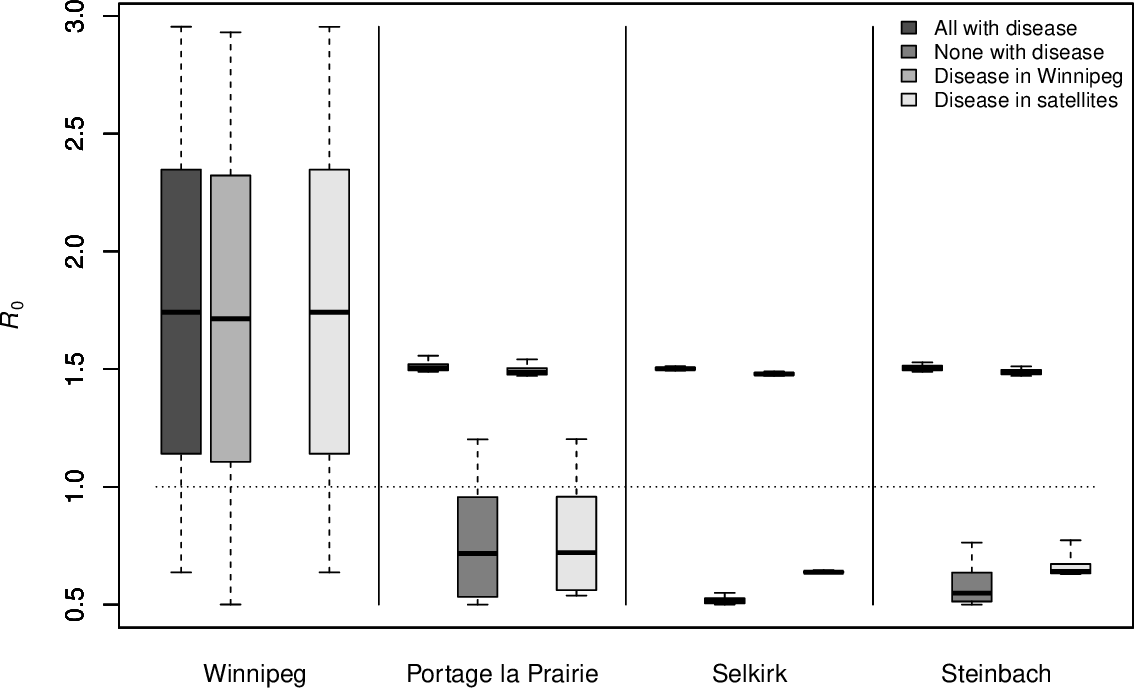
\includegraphics[width=\textwidth]{FIGS/sensitivity_4cities}
\end{center}
\emph{with disease}: $\mathcal{R}_0^x=1.5$; \emph{without disease}: $\mathcal{R}_0^x=0.5$. Each box and corresponding whiskers are 10,000 simulations
\end{frame}

\begin{frame}{Lower connectivity can drive $\mathcal{R}_0$}
	PLP and Steinbach have comparable populations but with parameters used, only PLP can cause the general $\mathcal{R}_0$ to take values larger than 1 when $\mathcal{R}_0^W<1$
	\vfill
	This is due to the movement rate: if $\mathcal{M}=0$, then
	$$
	\mathcal{R}_0=\max\{\mathcal{R}_0^W,\mathcal{R}_0^1,\mathcal{R}_0^2,\mathcal{R}_0^3\},
	$$
	since $FV^{-1}$ is then block diagonal
	\vfill
	Movement rates to and from PLP are lower $\rightarrow$ situation closer to uncoupled case and $\mathcal{R}_0^1$ has more impact on the general $\mathcal{R}_0$
\end{frame}

\begin{frame}{$\mathcal{R}_0$ does not tell the whole story!}
\begin{center}
	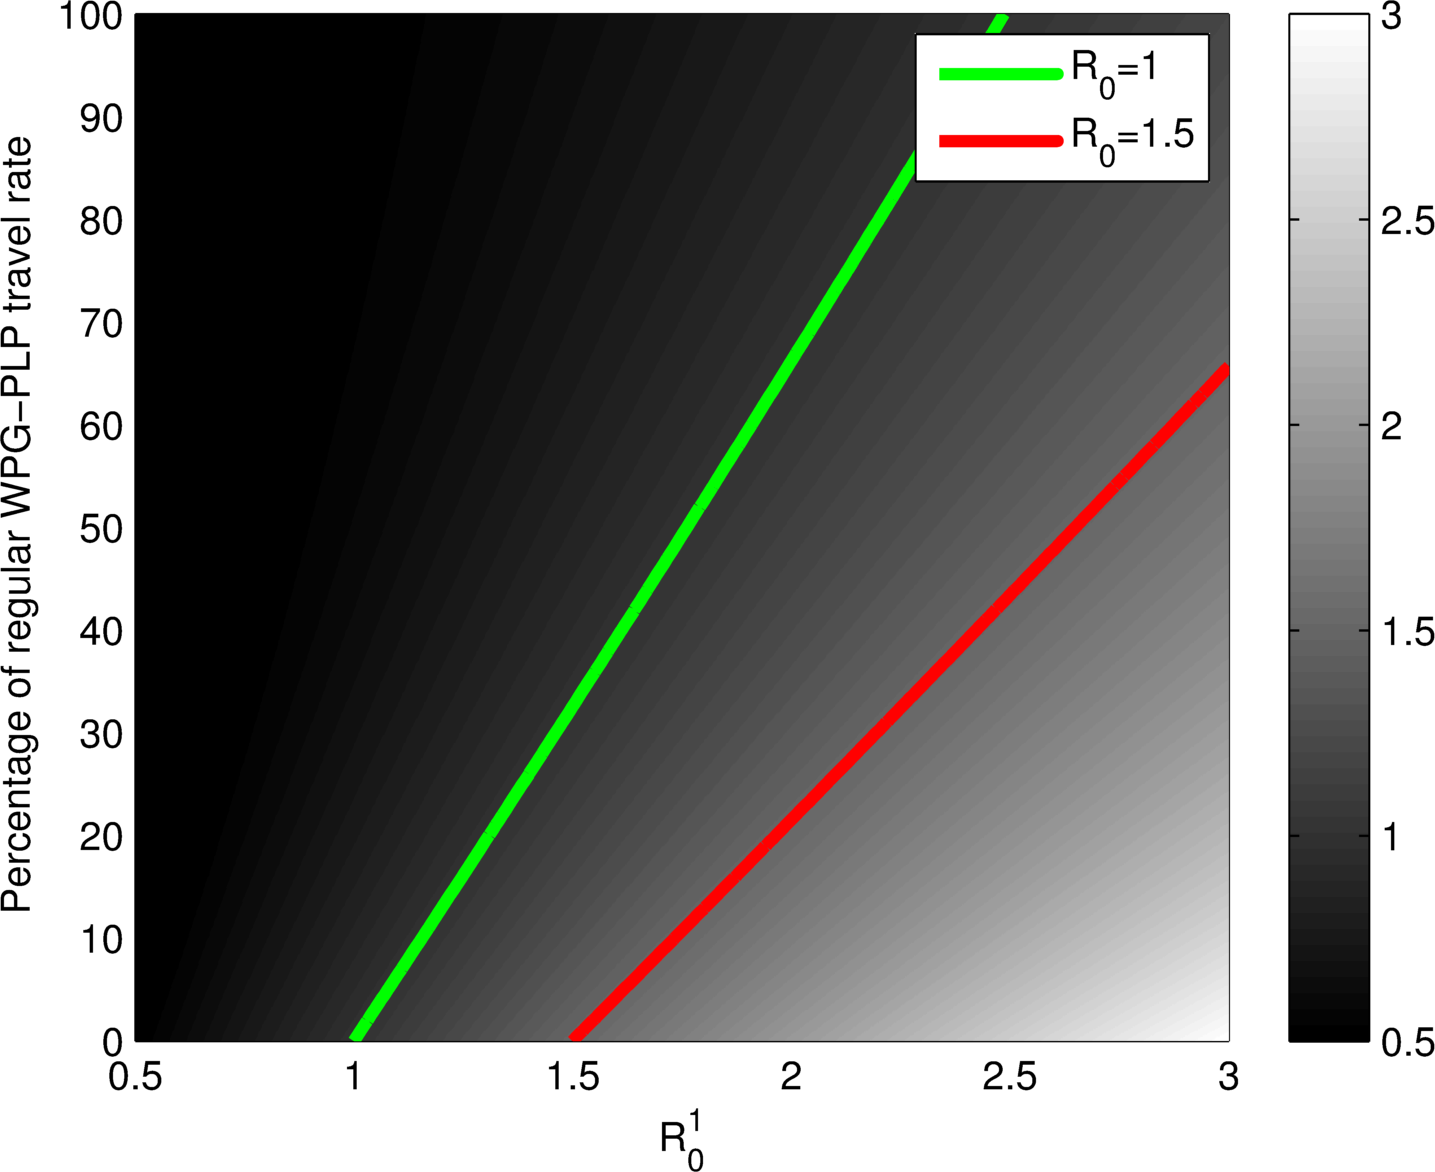
\includegraphics[width=0.49\textwidth]{FIGS/invasion_WPG_from_satellites_R01_m_caseR0W05_R0}
	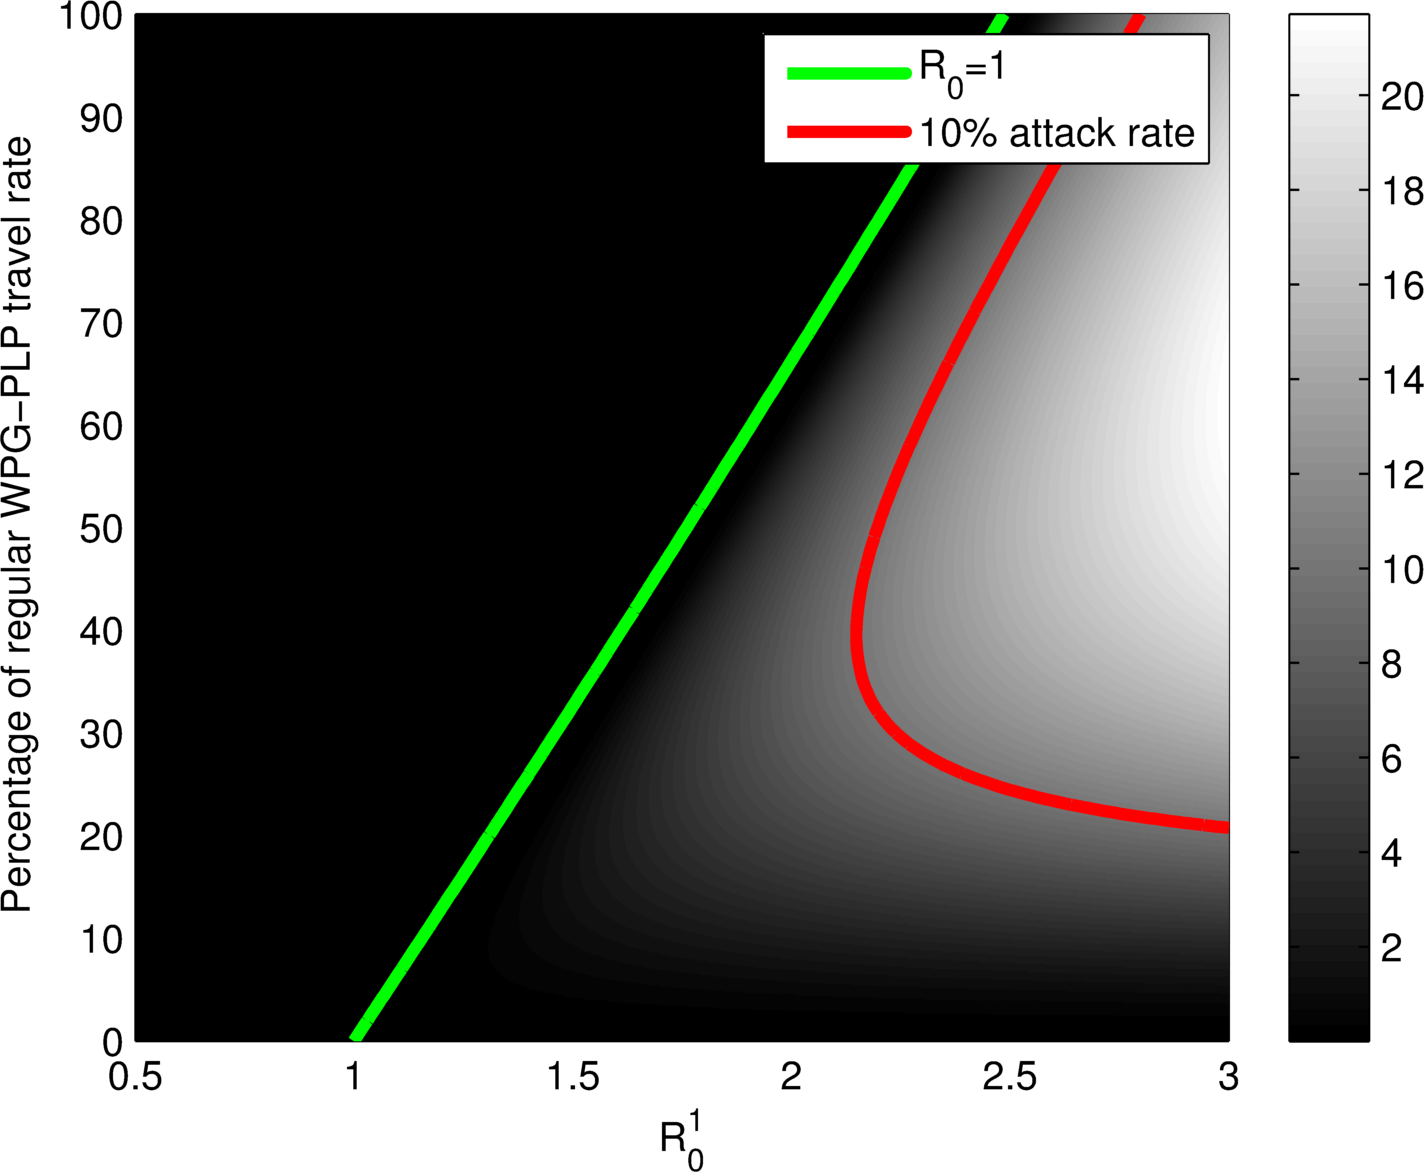
\includegraphics[width=0.49\textwidth]{FIGS/invasion_WPG_from_satellites_R01_m_caseR0W05_attackRate}
\end{center}
\vfill
Plots as functions of $\mathcal{R}_0^1$ in PLP and the reduction of movement between Winnipeg and PLP. Left: general $\mathcal{R}_0$. Right: Attack rate in Winnipeg
\end{frame}

% \frame{\frametitle{General SEIRS}
% System \eqref{sys:pSEIRS} with a generic force of infection.

% Order the infected variables as $E_{1},\ldots ,E_{|\P|},I_{1},\ldots,I_{|\P|}$. 

% Form the vectors
% \[
% \mathcal{F}=
% \begin{pmatrix}
% \Phi_1\\
% \vdots\\
% \Phi_{|\P|}\\
% 0\\
% \vdots\\
% 0
% \end{pmatrix},
% \] 
% representing new infections into the infected classes $E_{1},\ldots ,E_{|\P|},I_{1},\ldots,I_{|\P|}$,
% } 

% \frame{
% \[
% \mathcal{V}=-
% \begin{pmatrix}
% -(\varepsilon_1+d_1)E_1+\sum_{j=1}^{|\P|}m_{1j}^EE_j-\sum_{j=1}^{|\P|}m_{j1}^EE_1 \\
% \vdots\\
% -(\varepsilon_{|\P|}+d_{|\P|})E_{|\P|}+\sum_{j=1}^{|\P|}m_{{|\P|}j}^EE_j-\sum_{j=1}^{|\P|}m_{j{|\P|}}^EE_{|\P|}\\
% \varepsilon_1E_1-(\gamma_1+d_1+\delta_1)I_1+\sum_{j=1}^{|\P|}m_{1j}^II_j-\sum_{j=1}^{|\P|}m_{j1}^II_1\\
% \vdots\\
% \varepsilon_{|\P|}E_{|\P|}-(\gamma_{|\P|}+d_{|\P|}+\delta_{|\P|})I_{|\P|}+\sum_{j=1}^{|\P|}m_{{|\P|}j}^II_j-\sum_{j=1}^{|\P|}m_{j{|\P|}}^II_{|\P|}
% \end{pmatrix},
% \]
% representing other flows within and out off the infected classes $E_{1},\ldots ,E_{|\P|},I_{1},\ldots,I_{|\P|}$ (note that $\mathcal{V}$ has a minus sign).
% }

% \frame{
% \begin{itemize}
% \item
% Matrix of new infections $F$ and matrix of transfer between
% compartments $V$ are Jacobian matrices obtained by differentiating $\mathcal{F}$ and $\mathcal{V}$ with respect to the infected variables, evaluated at the disease free equilibrium (DFE).
% \end{itemize}
% Note that
% \[
% \frac{\partial\Phi_i}{\partial E_i}=\phi_i(S_i,I_i)\frac{\partial\beta_i}{\partial E_i}(N_i),
% \]
% and since $\phi=0$ at the DFE, it follows that $\partial\Phi_i/\partial E_i=0$ at the DFE.
% }

% \frame{
% Therefore, $F$ and $V$ are given in partitioned form by
% \begin{equation}\label{eq:FV_R0_pSEIRS}
% F=
% \begin{bmatrix}
% 0 & F_{12} \\ 
% 0 & 0%
% \end{bmatrix}%
% \text{ and }V=%
% \begin{bmatrix}
% V_{11} & 0 \\ 
% -V_{21} & V_{22}%
% \end{bmatrix}
% \end{equation}
% with
% \[
% F_{12}=\diag\left(\left.\frac{\partial \Phi_i}{\partial I_i}\right|_{DFE}\right),
% \]
% and
% \[
% V_{11}=-M_{{}}^{E}+\diag(\varepsilon
% _{i}+d_{i}+\dsum\limits_{j=1}^{|\P|}m_{ji}^{E})\quad 
% V_{21}=\diag\left( \varepsilon _{i}\right)
% \]
% \[
% V_{22}=-M_{{}}^{I}+\diag(\gamma
% _{i}+d_{i}+\delta_i+\dsum\limits_{j=1}^{|\P|}m_{ji}^{I}).
% \]
% }

% \frame{
% Matrices $V_{11}$ and $V_{22}$ are $|\P|\times|\P|$ irreducible 
% M-matrices and thus have positive inverses. 

% The next generation matrix%
% \begin{equation*}
% FV^{-1}=%
% \begin{bmatrix}
% F_{12}V_{22}^{-1}V_{21}V_{11}^{-1} & F_{12}V_{22}^{-1} \\ 
% 0 & 0%
% \end{bmatrix}%
% \end{equation*}%
% has spectral radius, denoted by $\rho $, given by $\rho \left(
% FV^{-1}\right) =\rho \left( F_{12}V_{22}^{-1}V_{21}V_{11}^{-1}\right)$. 
% }

% \frame{
% Jacobian matrix of the infected compartments at the
% DFE, $F-V$, has all eigenvalues with negative real parts
% if and only if $\rho \left( FV^{-1}\right) <1$. 

% This is summarized in the following theorem.
% \begin{theorem}\label{th:R0_pSEIRS}
% Define the \textit{basic reproduction number} $\R_0$ for system \eqref{sys:pSEIRS} with force of infection \eqref{eq:Phi_nSEIRSgeneral_generic} by
% \begin{equation}\label{eq:R0_pSEIRS}
% \R_0=\rho\left(FV^{-1}\right)=\rho \left( F_{12}V_{22}^{-1}V_{21}V_{11}^{-1}\right),
% \end{equation}
% with matrices $F$ and $V$ defined by \eqref{eq:FV_R0_pSEIRS}.
% Then the DFE is locally asymptotically stable if $\R_0<1$, and unstable if $\R_0>1$.
% \end{theorem} 
% }

% \frame{\frametitle{Case of proportional incidence}
% With a force of infection using standard (proportional) incidence, $\Phi=\beta_i S_iI_i/N_i$,
% \[
% \left.\frac{\partial\Phi_i}{\partial I_i}\right|_{DFE}=\beta_i\frac{S_i^*}{N_i^*}=\beta_i,
% \]
% so 
% \begin{itemize}
% \item $V$ unchanged
% \item $F_{12}=\diag(\beta_1,\ldots,\beta_{|\P|})$ provided that $\B_i(N_i)$ is such that $S_i^*=N_i^*$ (as is the case for example if $\B_i(N_i)=d_iN_i$). 
% \end{itemize}
% $\Rightarrow$ $\R_0$ does not depend on the movement parameters, only on the within-location parameters.
% }


% \frame{\frametitle{SEIRS with multiple species}
% Suppose $\B_{sp}$ are such that for all $s=1,\ldots,|\C|$ and $p=1,\ldots,|\P|$, $\lim_{t\to\infty}N_{sp}(t)=N_{sp}^*>0$.
 
% Method for multiple species is essentially the same as for a single species.

% To determine the matrices $F$ and $V$, order the state variables by
% species, then by location, \emph{i.e.}, 
% \begin{displaymath}
% E_{11},E_{21},\ldots,E_{|\C|1},E_{12},\ldots,E_{|\C||\P|},
% I_{11},I_{21},\ldots,I_{|\C|1},I_{12},\ldots,I_{|\C||\P|}.
% \end{displaymath}
% }

% \frame{
% The vector $\mathcal{F}$ then takes the form
% \[
% \mathcal{F}=
% \begin{pmatrix}
% \Phi_{11}\\
% \Phi_{21}\\
% \vdots\\
% \Phi_{|\C|1}\\
% \Phi_{21}\\
% \vdots\\
% \Phi_{|\C||\P|}\\
% 0\\
% \vdots\\
% 0
% \end{pmatrix},
% \]
% with the lower block of zeros consisting of $|\C||\P|$ zeros corresponding to the $I$ variables. 
% }

% \frame{
% At the DFE, $\partial\Phi_{sp}/\partial E_{ij}=0$, for all $s,i=1,\ldots,|\C|$ and all $p,j=1,\ldots,|\P|$. 

% Also, $\partial\Phi_{sp}/\partial I_{ij}=0$ for $s,i=1,\ldots,|\C|$ and all $p,j=1,\ldots,|\P|$, whenever $p\neq i$ (there are no contacts outside of the location).

% Then the nonnegative matrix $F$ takes the form
% \begin{displaymath}
% F=\begin{pmatrix}
% 0 & G \\
% 0 & 0 
% \end{pmatrix}
% =
% \begin{pmatrix}
% \hbox{\LARGE $0$} & \bigoplus\limits_{k=1}^{|\P|} G_k \\
% \hbox{\LARGE $0$} & \hbox{\LARGE $0$} 
% \end{pmatrix},
% \end{displaymath}
% with $G_k$ an $|\C|\times |\C|$-matrix with $(i,j)$ entry equal to
% \[
% [G_k]_{ij}=\left.\frac{\partial\Phi_{ik}}{\partial I_{jk}}\right|_{DFE}.
% \] 
% }

% \frame{
% The matrix $V$ is the block matrix
% \begin{displaymath}
% V=\begin{pmatrix}
% A & 0 \\
% -C & B
% \end{pmatrix}
% =\begin{pmatrix}
% \begin{matrix}
% A_{11} & \cdots & A_{1|\P|} \\
% \vdots & \ddots & \vdots \\
% A_{|\P|1} & \cdots & A_{|\P||\P|}
% \end{matrix}
% & \hbox{\LARGE $0$} \\
% -\bigoplus\limits_{k=1}^{|\P|}C_k &
% \begin{matrix}
% B_{11} & \cdots & B_{1|\P|} \\
% \vdots & \ddots & \vdots \\
% B_{|\P|1} & \cdots & B_{|\P||\P|}
% \end{matrix}
% \end{pmatrix}
% \end{displaymath}
% }


% \frame{
% Matrix $A$ is the block matrix $A=A_{jk}$, with each $A_{jk}$ block an
% $|\C|\times|\C|$ diagonal matrix. 
% The $(i,i)$ entry of $A_{kk}$ is equal to
% $d_{ik}+\varepsilon_{ik}+\sum_{l=1}^{|\P|} m_{ilk}$, whereas for $j\neq k$
% the $(i,i)$ entry of $A_{jk}$ is $-m_{ijk}$. 
% Matrix $B$ is the same as $A$ but with $\varepsilon_{ik}$ replaced by
% $\gamma_{ik}$. 
% Finally, $C_k$ is an $s\times s$
% diagonal matrix with $(i,i)$ entry equal to $\varepsilon_{ik}$.

% Matrices $G$, $A$, $B$ and $C$ are $|\C||\P|\times |\C||\P|$-matrices. 
% Matrices $A$ and $B$ are nonsingular $M$-matrices since they have the
% Z-sign pattern and are diagonally dominant by columns. Thus $A^{-1}$ and $B^{-1}$ are
% nonnegative. 
% }

% \frame{
% Due to the particular structure of $F$ and $V$, the computation of
% $\rho(FV^{-1})$ is greatly simplified. 
% Indeed, the inverse $V^{-1}$ of $V$ keeps its block triangular
% structure 
% \begin{displaymath}
% V^{-1}=\begin{pmatrix}
% A^{-1} & 0 \\
% B^{-1}CA^{-1} & B^{-1}
% \end{pmatrix},
% \end{displaymath}
% and it follows that
% \begin{displaymath}
% FV^{-1}=
% \begin{pmatrix}
% 0 & G\\
% 0 & 0 
% \end{pmatrix}
% \begin{pmatrix}
% A^{-1} & 0 \\
% B^{-1}CA^{-1} & B^{-1}
% \end{pmatrix}
% =
% \begin{pmatrix}
% GB^{-1}CA^{-1} & GB^{-1} \\
% 0 & 0
% \end{pmatrix}.
% \end{displaymath}
% Thus
% \begin{displaymath}
% \R_0=\rho(GB^{-1}CA^{-1})
% \end{displaymath}
% }

% \frame{
% Since $GB^{-1}CA^{-1}$ is a nonnegative matrix,
% its spectral radius is attained at the largest real eigenvalue.
% If $\R_0<1$, then the DFE is locally stable, whereas
% if $\R_0>1$, then the DFE is unstable. The following result has been proved.
% \begin{theorem}\label{th:R0_spSEIRS_LAS}
% For system \eqref{sys:spSEIRS} with $|\C|$ species and $\bar n$ locations,
% \begin{equation}\label{eq:R0_spSEIRS}
% \R_0=\rho(GB^{-1}CA^{-1})
% \end{equation}
% If $\R_0<1$, then the DFE is locally asymptotically stable, if $\R_0>1$
% then the DFE is unstable.
% \end{theorem}
% }

% \frame{\frametitle{Case of proportional incidence}
% In the case of a force of infection with proportional incidence, the $(i,j)$ entry of $G_k$ takes the form $\beta_{ijk}\hat S_{ik}/N^*_{jk}$.
% }



% \frame{\frametitle{SEIRS with residency location}
% Order the infected variables (exposed and infectives) as 
% \[
% E_{11},\ldots,E_{1|\P|}, E_{21},\ldots E_{2|\P|},\ldots
% E_{|\P||\P|},I_{11},\ldots,I_{1|\P|}, I_{21},\ldots I_{2|\P|},\ldots,
% I_{|\P||\P|}.
% \]

% Since $\Phi_{ij}$ describes the infection of susceptible residents of location $i$ who are currently in location $j$, there holds that $\partial \Phi_{pq}/\partial I_{ij}=0$ if $q\neq j$, for all $i,j,p,q=1,\ldots,|\P|$, since contacts only involve individuals that are in the same location.
% }

% \frame{
% This gives the block matrix $F$,
% \[
% F=\begin{pmatrix}
% 0 & G \\
% 0 & 0
% \end{pmatrix}
% \]
% where $G$ is an $|\P|^2\times|\P|^2$ matrix having $|\P|^2$ blocks, with each
% block $G_{ij}$ an $|\P|\times|\P|$
% diagonal matrix of the form $G_{ij}=\diag(g_{ijq})$, where 
% $g_{ijq}=\beta_{ijq} \hat N_{iq} /\hat N^p_{q}$, for
% $q=1,\ldots,|\P|$.
% \[
% G_{ij}=\diag
% \left(
% \left.\frac{\partial\Phi_{i1}}{\partial I_{j1}}\right|_{DFE},\left.\frac{\partial\Phi_{i2}}{\partial I_{j2}}\right|_{DFE},\ldots,\left.\frac{\partial\Phi_{i|\P|}}{\partial I_{j|\P|}}\right|_{DFE}
% \right).
% \]
% }

% \frame{
% Also, $V$ is a lower triangular block matrix,
% \[
% V=\begin{pmatrix}
% A & 0 \\
% C & B
% \end{pmatrix}
% =
% \begin{pmatrix}
% \bigoplus\limits_{p=1}^{|\P|}A_p & \hbox{\LARGE $0$} \\
% -\bigoplus\limits_{p=1}^{|\P|}C_p & \bigoplus\limits_{p=1}^{|\P|}B_p 
% \end{pmatrix}
% \] 
% where each block $A$, $B$ and $C$ is $|\P|^2\times|\P|^2$.
% }


% \frame{
% For $p=1,\ldots|\P|$, $A_p$ is an $|\P|\times|\P|$ matrix with
% \[
% A_p=
% \tiny
% \left[
% \begin{array}{ccccc}
% \varepsilon_{p1}+d_{p1}+\sum_{k=1}^{|\P|}m_{pk1}^E & -m_{p12}^E & -m_{p13}^E & \cdots & -m_{p1|\P|}^E \\
% -m_{p21}^E & \varepsilon_{p2}+d_{p2}+\sum_{k=1}^{|\P|}m_{pk2}^E & -m_{p23}^E & \cdots & -m_{p2|\P|}^E \\
% & & & \\
% -m_{p|\P|1}^E & -m_{p|\P|2}^E & -m_{p|\P|3}^E & \cdots & \varepsilon_{p|\P|}+d_{p|\P|}+\sum_{k=1}^{|\P|}m_{pk|\P|}^E
% \end{array}
% \right],
% \]
% }

% \frame{
% $B_p$ is an $|\P|\times|\P|$-matrix with
% \[
% B_p=\tiny
% \left[
% \begin{array}{ccccc}
% \gamma_{p1}+d_{p1}+\sum_{k=1}^{|\P|}m_{pk1}^I & -m_{p12}^I & -m_{p13}^I & \cdots & -m_{p1|\P|}^I \\
% -m_{p21}^I & \gamma_{p2}+d_{p2}+\sum_{k=1}^{|\P|}m_{pk2}^I & -m_{p23}^I & \cdots & -m_{p2|\P|}^I \\
% & & & \\
% -m_{p|\P|1}^I & -m_{p|\P|2}^I & -m_{p|\P|3}^I & \cdots & \gamma_{p|\P|}+d_{p|\P|}+\sum_{k=1}^{|\P|}m_{pk|\P|}^I
% \end{array}
% \right],
% \]
% and $C_p$ is an $|\P|\times|\P|$ diagonal matrix with $C_p=\diag(\varepsilon_{p1},\ldots,\varepsilon_{p|\P|})$.
% }

% \frame{
% Since $A_k$ and $B_k$ have the Z-sign pattern and have all positive
% column sums, $A_k$ and $B_k$ are nonsingular M-matrices. Note that
% \[
% \left(\bigoplus\limits_{p=1}^{|\P|}\left(B_p\right)^{-1}\right)
% \left(\bigoplus\limits_{p=1}^{|\P|}\left(C_p\right)\right)
% \left(\bigoplus\limits_{p=1}^{|\P|}\left(A_p\right)^{-1}\right)
% =\bigoplus\limits_{p=1}^{|\P|}\left(A_pC_p^{-1}B_p\right)^{-1}.
% \]
% }

% \frame{
% Therefore, the inverse of $V$ is the nonnegative matrix
% \begin{equation}\label{eq:invV_ppSEIRS}
% V^{-1}=
% \begin{pmatrix}
% \bigoplus\limits_{p=1}^{|\P|}\left(A_p\right)^{-1} & \hbox{\LARGE $0$} \\
% \bigoplus\limits_{p=1}^{|\P|}\left(A_pC_p^{-1}B_p\right)^{-1}
% & \bigoplus\limits_{p=1}^{|\P|}\left(B_p\right)^{-1}
% \end{pmatrix}.
% \end{equation}
% }

% \frame{
% Since $V^{-1}$ is lower triangular by blocks, $FV^{-1}$ can be given
% by blocks.
% The basic reproduction number
% for system (\ref{sys:ppSEIRS}) is 
% \begin{equation}
% \R_0=\rho
% \left\{
% G \left(
% \bigoplus\limits_{p=1}^{|\P|}
% (A_p)C_p^{-1}(B_p)\right)^{-1}
% \right\}
% \label{eq:R0}
% \end{equation} 
% where $\rho\{\cdot\}$ is the spectral radius, and the following result
% holds.
% \begin{theorem}
% Let $\R_0$ be defined as in (\ref{eq:R0}). If $\R_0<1$, then the
% DFE of (\ref{sys:ppSEIRS}) is locally asymptotically stable. 
% If $\R_0>1$, then the DFE of (\ref{sys:ppSEIRS}) is unstable.
% \label{th:R0}
% \end{theorem}
% }

%%%%%%%%%%%%%%%%%%%
%%%%%%%%%%%%%%%%%%%
%%%%%%%%%%%%%%%%%%%
%%%%%%%%%%%%%%%%%%%
%%%%%%%%%%%%%%%%%%%
%%%%%%%%%%%%%%%%%%%
\subsection{Global stability of the DFE when $\R_0<1$}
\newSubSectionSlide{FIGS-slides-admin/Gemini_Generated_Image_vqpscpvqpscpvqps.jpeg}

\frame{\frametitle{The toy $|\P|$-SLIRS}
LAS results for $\R_0<1$ can sometimes be strengthened to GAS. One class of models where this works often is when the population is either constant or asymptotically constant and incidence is \emph{standard}
\vfill
\begin{theorem}\label{th:pSLIRS_GAS}
Let $\R_0$ be defined as in Theorem~\ref{th:LAS_DFE_pSLIRS_toy} and use proportional incidence $\Phi_p=\beta_pS_pI_p/N_p$. If $\R_0<1$, then the DFE of system \eqref{sys:pSLIRS_toy} is globally asymptotically stable
\end{theorem}
}



\frame{\frametitle{$|\S|\;|\P|$-SLIRS with multiple species}
In the case in which movement is equal for all compartments and there is no disease death, a comparison theorem argument can be used as in Theorem~\ref{th:pSLIRS_GAS} to show that if $\R_0<1$, then the
DFE of the $|\S|\;|\P|$-SLIRS \eqref{sys:spSLIRS} is globally asymptotically stable. 
\vfill
\begin{theorem}\label{th:R0_spSEIRS_GAS}
For system \eqref{sys:spSLIRS} with $|\S|$ species and $|\P|$ locations, with movement equal for all compartments, define $\R_0$ appropriately and use proportional incidence. 
If $\R_0<1$, then the DFE is globally asymptotically stable
\end{theorem}
}



%%%%%%%%%%%%%%%%%%%
%%%%%%%%%%%%%%%%%%%
\subsection{Metapopulation-specific problems}
\newSubSectionSlide{FIGS-slides-admin/Gemini_Generated_Image_vqpscpvqpscpvqps.jpeg}

\begin{frame}{Metapopulation-specific problems -- Two main types}
\begin{itemize}
	\item \textbf{Inheritance problems --} Which of the properties of the constituting units are inherited by the metapopulation?
	\vfill
	\item \textbf{Metapopulation-specific behaviours --} Are there dynamic behaviours observed in a metapopulation not observed in the constituting units?
\end{itemize}
\end{frame}


\begin{frame}{Inherited dynamical properties (a.k.a. I am lazy)}
	Given
	\begin{subequations}
		\begin{align}
			s_{kp}' &= f_{kp}(S_p,I_p) \label{sys:generic_intra_ds} \\
			i_{\ell p}' &= g_{\ell p}(S_p,I_p) \label{sys:generic_intra_di}
		\end{align}				
	\end{subequations}
	with known properties, what is known of
	\begin{subequations}
		\begin{align}
			s_{kp}' &= f_{kp}(S_p,I_p)+\textstyle{\sum_{q\in\mathcal{P}}} m_{kpq}s_{kq} 
			\label{sys:generic_inter_ds} \\
			i_{\ell p}' &= g_{\ell p}(S_p,I_p)+\textstyle{\sum_{q\in\mathcal{P}}} m_{\ell pq}i_{\ell q}
			\label{sys:generic_inter_di}
		\end{align}				
	\end{subequations}
	\begin{itemize}
		\item Existence and uniqueness $\checkmark$
		\item Invariance of $\mathbb{R}_+^\bullet$ under the flow $\checkmark$
		\item Boundedness $\checkmark$
		\item Location of individual $\mathcal{R}_{0i}$ and general $\mathcal{R}_0$ ?
		\item GAS ?		
	\end{itemize}
	- 
\end{frame}

\begin{frame}{An inheritance problem -- Backward bifurcations}
	\begin{itemize}
		\item Suppose a model that, isolated in a single patch, undergoes so-called backward bifurcations
		\item This means the model admits subthreshold endemic equilibria
		\item What happens when you couple many such consistuting units?
	\end{itemize}
	\vfill
	\emph{YES}, coupling together backward bifurcating units can lead to a system-level backward bifurcation
	\vfill
	JA, Ducrot \& Zongo. \href{https://julien-arino.github.io/assets/pdf/papers/2012_ArinoDucrotZongo-JMB64.pdf}{A metapopulation model for malaria with transmission-blocking partial immunity in hosts}. \emph{Journal of Mathematical Biology} \textbf{64}(3):423-448 (2012) 		
\end{frame}

\begin{frame}{Metapopulation-induced behaviours ?}
	``Converse'' problem to inheritance problem. Given
	\begin{align}
	s_{kp}' &= f_{kp}(S_p,I_p)  \tag{9a} \\
	i_{\ell p}' &= g_{\ell p}(S_p,I_p) \tag{9b}
	\end{align}
	with known properties, does
	\begin{align}
	s_{kp}' &= f_{kp}(S_p,I_p)+\textstyle{\sum_{q\in\mathcal{P}}} m_{kpq}s_{kq}  \tag{10a} \\
	i_{\ell p}' &= g_{\ell p}(S_p,I_p)+\textstyle{\sum_{q\in\mathcal{P}}} m_{\ell pq}i_{\ell q}  \tag{10b}
	\end{align}
	exhibit some behaviours not observed in the uncoupled system?
	
	E.g.: units have $\{\mathcal{R}_0<1\implies$ DFE GAS, $\mathcal{R}_0>1\implies$ 1 GAS EEP$\}$ behaviour, metapopulation has periodic solutions
		
\end{frame}

\begin{frame}{Mixed equilibria}
	Can there be situations where some locations are at the DFE and others at an EEP?
	\vfill
	This is the problem of \textbf{mixed equilibria}
	\vfill
	This is a metapopulation-specific problem, not one of inheritance of dynamical properties!
\end{frame}

\begin{frame}{Types of equilibria}
	\begin{definition}[Location level EP]
		Location $p\in\mathcal{P}$ at equilibrium is \textbf{empty} if $X_p^\star=0$, at the \textbf{disease-free equilibrium} if $X_p^\star=(s_{k_1p}^\star,\ldots,s_{k_up}^\star,0,\ldots,0)$, where $k_1,\ldots,k_u$ are some indices with $1\leq u\leq|\mathcal{U}|$ and $s_{k_1p}^\star,\ldots,s_{k_up}^\star$ are positive, and at an \textbf{endemic equilibrium} if $X_p\gg 0$
	\end{definition}
	\vfill
	\begin{definition}[Metapopulation level EP]
		A \textbf{population-free equilibrium} has all locations empty. A \textbf{metapopulation disease-free equilibrium} has all locations at the disease-free equilibrium for the same compartments. A \textbf{metapopulation endemic equilibrium} has all locations at an endemic equilibrium
	\end{definition}
\end{frame}

\begin{frame}{Mixed equilibria}
	\begin{definition}
		A \textbf{mixed equilibrium} is an equilibrium such that
		\begin{itemize}
			\item all locations are at a disease-free equilibrium but the system is not at a metapopulation disease-free equilibrium
			\item or, there are at least two locations that have different types of location-level equilibrium (empty, disease-free or endemic)
		\end{itemize}
	\end{definition}
	E.g., 
	$$
	((S_1,I_1,R_1),(S_2,I_2,R_2))=((+,0,0),(+,+,+))
	$$
	is mixed and so is
	$$
	((S_1,I_1,R_1),(S_2,I_2,R_2))=((+,0,0),(+,0,+))
	$$
\end{frame}


\begin{frame}
Notation is specific here: $p\in\P$, $\A(p)$ and $\D(p)$ are the ancestry and descendents of $p$ in the movement digraph
	\begin{theorem}
		Suppose that movement is similar for all compartments (MSAC) and that the system is at equilibrium
		\begin{itemize}
			\item If patch $p\in\mathcal{P}$ is empty, then all patches in $\mathcal{A}(p)$ are empty 
			\item If patch $p\in\mathcal{P}$ is at a disease free equilibrium, then the subsystem consisting of all patches in $\{p,\mathcal{A}(p)\}$ is at a metapopulation disease free equilibrium 
			\item If patch $p\in\mathcal{P}$ is at an endemic equilibrium, then all patches in $\mathcal{D}(p)$ are also at an endemic equilibrium
			\item If $\mathcal{G}^c$ is strongly connected for some compartment $c\in\mathcal{C}$, then there does not exist mixed equilibria
		\end{itemize}
	\end{theorem}
	Note that MSAC $\implies$ $\mathcal{A}^c=\mathcal{A}$ and $\mathcal{D}^c=\mathcal{D}$ for all $c\in\mathcal{C}$
\end{frame}




% \frame{\frametitle{Similar movement}
% What is important here is not that movement be status-independent, but that different states have the same connection graph (irrespective of the movement rates).
% \begin{definition}\label{def:similar_movement}
% Movement in system \eqref{sys:pSEIRS} is similar for all states if, for all $i,j=1,\ldots,|\P|$, there holds that either
% \[
% m_{ij}^Sm_{ij}^Em_{ij}^Im_{ij}^R>0
% \]
% or
% \[
% m_{ij}^S=m_{ij}^E=m_{ij}^I=m_{ij}^R=0.
% \]
% Movement in system \eqref{sys:spSEIRS} is similar for all states if, for all $i,j=1,\ldots,|\P|$ and a given species $c\in\C$, there holds that either
% \[
% m_{sij}^Sm_{sij}^Em_{sij}^Im_{sij}^R>0
% \]
% or
% \[
% m_{sij}^S=m_{sij}^E=m_{sij}^I=m_{sij}^R=0.
% \]
% If this is true for all states and all species, then movement in \eqref{sys:spSEIRS} is similar for all states and all species.
% Movement in system \eqref{sys:ppSEIRS} is similar for all states if, for all $i,j,k=1,\ldots,|\P|$, there holds that either
% \[
% m_{ijk}^Sm_{ijk}^Em_{ijk}^Im_{ijk}^R>0
% \]
% or
% \[
% m_{ijk}^S=m_{ijk}^E=m_{ijk}^I=m_{ijk}^R=0.
% \]
% \end{definition}
% }


% \frame{\frametitle{Movement similar for all states -- Model with normal movement}
% System with multiple species \eqref{sys:spSEIRS}. Specialization to the case of a single species is trivial.

% \begin{theorem}\label{th:DFE_propagates_spSEIRS}
% Suppose that \eqref{sys:spSEIRS} with movement similar for all states is at an equilibrium. 

% If a given location $p$ is at a DFE, then all locations that have an access to location $p$ for a given species $s$ are also at a DFE.
% \end{theorem}
% }

% \frame{\frametitle{Proof}
% Fix the species index at $s$. For simplicity suppose that $p=1$, i.e., there is no disease in location 1. Thus $E_{s1}=I_{s1}=0$. Then for $p=1$, \eqref{sys:spSEIRS_Isp} is
% \[
% 0=\frac{d}{dt}I_{s1}=\sum_{r=2}^{|\P|}m_{s1r}I_{sr}.
% \]
% For a given location $r$, define
% \[
% \mathcal{P}_{\to r}=\{q:m_{srq}>0\},
% \]
% the subset of locations with a direct access to location $r$, and
% \[
% \mathcal{P}_{\not\to r}=\{q\neq r: m_{srq}=0\},
% \]
% the subset of locations with no direct access to location $r$. 
% }

% \frame{
% Then, since $I_{sr}\geq 0$ and
% \[
% \sum_{r=2}^{|\P|}m_{s1r}I_{sr}=\sum_{r\in\mathcal{P}_{\to 1}}m_{s1r}I_{sr}+
% \sum_{r\in\mathcal{P}_{\not\to 1}}m_{s1r}I_{sr}=0,
% \]
% it follows that $I_{sr}=0$ for $r\in\mathcal{P}_{\to 1}$. Similarly, setting $p=1$ in \eqref{sys:spSEIRS_Esp} and using $\mathcal{P}_{\to 1}$, it follows that $E_{sr}=0$ for $r\in\mathcal{P}_{\to 1}$. Thus, all locations $r$ with a direct access to location 1 have no disease, i.e., are such that $E_{sr}=I_{sr}=0$.


% Now consider a location $r$ in $\mathcal{P}_{\to 1}$. Using the same argument as previously, it follows that $E_{sw}=I_{sw}=0$ for all $w\in\mathcal{P}_{\to r}$. locations that are in $\mathcal{P}_{\to r}\setminus\mathcal{P}_{\to 1}$ have a length 2 access to location 1. By induction, all locations in $\overline{\mathcal{P}}_{\to 1}$ are at the DFE if location 1 is at the DFE.
% }

% \frame{
% \begin{itemize}
% \item
% This result is independent of the nature of the birth function $\B_{sp}$. 
% \item Conclusions have not been derived on the nature of $R_p$ for those locations that are at the DFE, nor has it been shown that $S_p\to N_p^*$. 
% \item In fact, with a little additional work, it can be shown that $\lim_{t\to\infty}R_k(t)=0$ for $k\in\overline{\mathcal{P}}_{\to p}$. In this case, $S_p\to N_p^*$, with the precise value of $N_p^*$ undetermined until a birth function has been chosen.
% \end{itemize}
% }

% \frame{
% \begin{theorem}\label{th:EEP_propagates_spSEIRS}
% Suppose that \eqref{sys:spSEIRS} with movement similar for all states is at an equilibrium. 

% If a given location $p$ is at an endemic equilibrium, then all locations that can be accessed from location $p$ for a given species $s$ are also at an endemic equilibrium.
% \end{theorem}
% }

% \frame{\frametitle{Proof}
% Fix the species index $s$. For simplicity suppose that $p=1$, i.e., $E_{s1}+I_{s1}>0$. From \eqref{sys:spSEIRS_Esp} and \eqref{sys:spSEIRS_Isp} with $q\neq 1$,
% \begin{align*}
% 0=\frac{d}{dt}(E_{sq}+I_{sq}) &= \Phi_{sq}-d_{sq}(E_{sq}+I_{sq})-\gamma_{sq}I_{sq} \\
% &\quad +\sum_{r=1}^{|\P|}m_{sqr}(E_{sr}+I_{sr})-\sum_{r=1}^{|\P|}m_{srq}(E_{sq}+I_{sq}).
% \end{align*}
% Assume that $E_{sq}+I_{sq}=0$ and $m_{sq1}>0$, i.e., location 1 has access to location $q$. Then the above equation reduces to 
% \[
% 0=\sum_{r=1}^{|\P|}m_{sqr}(E_{sr}+I_{sr}),
% \]
% and implies that $E_{s1}+I_{s1}=0$, giving a contradiction. Thus the disease in location $q$ is at an endemic equilibrium. The remainder of the proof follows as in the proof of Theorem~\ref{th:DFE_propagates_spSEIRS}.
% }

% %%%%%%%%%%%%%%%
% \frame{\frametitle{Movement similar for all states -- Model with residency location}
% \begin{theorem}\label{th:DFE_propagates_ppSEIRS}
% Suppose that system \eqref{sys:ppSEIRS} with movement similar for all states is at an equilibrium, and that a given location $p$ is at the DFE. 

% Then all locations that can be accessed from location $p$, and all locations that have an access to location $p$, are at the DFE.
% \end{theorem}
% }

% \frame{\frametitle{Proof}
% Suppose, without loss of generality, that location $1$ is at the DFE, i.e., $I_{k1}=E_{k1}=0$ for all $k=1,\ldots,|\P|$. 

% Then consider \eqref{sys:ppSEIRS_Eij} and \eqref{sys:ppSEIRS_Iij} with $i=1$. Since $I_{11}=0$, it follows that $\Phi_{11}=0$ and thus
% \begin{align*}
% \frac{d}{dt}E_{11} &= \sum_{k=1}^{|\P|} m_{11k}^E E_{1k} \\
% \frac{d}{dt}I_{11} &= \sum_{k=1}^{|\P|} m_{11k}^I I_{1k}. 
% \end{align*}
% Recall that variables remain nonnegative. 

% Since the system is at equilibrium, $E_{1k}=0$ for all locations $k$ such that E individuals from location $k$ have direct access to location 1, and $I_{1k}=0$ for all locations $k$ such that I individuals from location $k$ have direct access to location 1. 
% }

% \frame{
% These sets of locations are denoted $\mathcal{P}_{\to 1}^E$ and $\mathcal{P}_{\to 1}^I$, respectively. Since movement is similar for all states, $\mathcal{P}_{\to 1}^E=\mathcal{P}_{\to 1}^I=:\mathcal{P}_{\to 1}$. 

% In summary, if location 1 is at the DFE, then there holds that for all locations $j$ in $\mathcal{P}_{\to 1}$, $E_{1j}=I_{1j}=0$, i.e., there is no disease in visitors from location 1 visiting locations that have direct access to location 1. 
% }

% \frame{
% Consider now \eqref{sys:ppSEIRS_Eij} for one of these locations, i.e., for $j\in\mathcal{P}_{\to 1}$. There holds, for visitors to $j$ from location 1,
% \[
% \frac{d}{dt}E_{1j} = \Phi_{1j}.
% \]
% Since the system is at an equilibrium, $\Phi_{1j}=0$, that is 
% \[
% 0=\Phi_{1j}=\sum_{k=1}^{|\P|}\phi_{1k}(S_{1j},I_{kj}).
% \]
% It was shown (Theorem~\ref{th:Spositive}) that $S_{ij}>0$ for all positive times, provided that $m_{ijk}>0$. Since the $S_{ij}$ are positive, there holds that for all $j\in\mathcal{P}_{\to 1}$ such that $m_{1jk}>0$,
% $I_{kj}=0$. Using the same type of argument that was used to show that $R=0$ in the proof of Theorem~\ref{th:R0_spSEIRS_GAS}, it follows that for these locations, there also holds that $E_{kj}=0$.

% To summarize, if location 1 is at the DFE, then locations $j\in\mathcal{P}_{\to 1}$ are also at the DFE. By induction, all locations that are in $\overline{\mathcal{P}}_{\to 1}$ are at the DFE.
% }




%%%%%%%%%%%%%%%%%%
%%%%%%%%%%%%%%%%%%
\subsection{Computational aspects of metapopulation models}
\newSubSectionSlide{FIGS-slides-admin/Gemini_Generated_Image_vqpscpvqpscpvqps.jpeg}

\begin{frame}
	\begin{itemize}
		\item JA. \href{https://doi.org/10.1016/j.idm.2017.05.001}{Spatio-temporal spread of infectious pathogens of humans}. \emph{Infectious Disease Modelling} \textbf{2}(2):218-228 (2017)
		\item JA. \href{https://doi.org/10.1016/j.idm.2019.12.008}{Mathematical epidemiology in a data-rich world}. \emph{Infectious Disease Modelling} \textbf{5}:161-188 (2020)
		\item github repo \href{https://github.com/julien-arino/modelling-with-data}{modelling-with-data}
	\end{itemize}
\end{frame}

\begin{frame}{Not very difficult}
As for the mathematical analysis: if you do things carefully and think about things a bit, numerics are not hard. Well: not harder than numerics in low-D
\vfill
Exploit vector structure
\end{frame}

\begin{frame}[fragile]{Set up parameters}
\begin{knitrout}
\definecolor{shadecolor}{rgb}{0.969, 0.969, 0.969}\color{fgcolor}\begin{kframe}
\begin{alltt}
\hldef{pop} \hlkwb{=} \hlkwd{c}\hldef{(}\hlnum{34.017}\hldef{,} \hlnum{1348.932}\hldef{,} \hlnum{1224.614}\hldef{,} \hlnum{173.593}\hldef{,} \hlnum{93.261}\hldef{)} \hlopt{*} \hlnum{1e+06}
\hldef{countries} \hlkwb{=} \hlkwd{c}\hldef{(}\hlsng{"Canada"}\hldef{,} \hlsng{"China"}\hldef{,} \hlsng{"India"}\hldef{,} \hlsng{"Pakistan"}\hldef{,} \hlsng{"Philippines"}\hldef{)}
\hldef{T} \hlkwb{=} \hlkwd{matrix}\hldef{(}\hlkwc{data} \hldef{=} \hlkwd{c}\hldef{(}\hlnum{0}\hldef{,} \hlnum{1268}\hldef{,} \hlnum{900}\hldef{,} \hlnum{489}\hldef{,} \hlnum{200}\hldef{,}
                    \hlnum{1274}\hldef{,} \hlnum{0}\hldef{,} \hlnum{678}\hldef{,} \hlnum{859}\hldef{,} \hlnum{150}\hldef{,}
                    \hlnum{985}\hldef{,} \hlnum{703}\hldef{,} \hlnum{0}\hldef{,} \hlnum{148}\hldef{,} \hlnum{58}\hldef{,}
                    \hlnum{515}\hldef{,} \hlnum{893}\hldef{,} \hlnum{144}\hldef{,} \hlnum{0}\hldef{,} \hlnum{9}\hldef{,}
                    \hlnum{209}\hldef{,} \hlnum{174}\hldef{,} \hlnum{90}\hldef{,} \hlnum{2}\hldef{,} \hlnum{0}\hldef{),}
           \hlkwc{nrow} \hldef{=} \hlnum{5}\hldef{,} \hlkwc{ncol} \hldef{=} \hlnum{5}\hldef{,} \hlkwc{byrow} \hldef{=} \hlnum{TRUE}\hldef{)}
\end{alltt}
\end{kframe}
\end{knitrout}
\end{frame}

\begin{frame}[fragile]{Computing birth and death rates}
Average life expectancy at birth (years): 81.30, 78.59, 67.74, 66.43, 72.19
\begin{knitrout}
\definecolor{shadecolor}{rgb}{0.969, 0.969, 0.969}\color{fgcolor}\begin{kframe}
\begin{alltt}
\hldef{pop} \hlkwb{=} \hlkwd{c}\hldef{(}\hlnum{34.017}\hldef{,} \hlnum{1348.932}\hldef{,} \hlnum{1224.614}\hldef{,} \hlnum{173.593}\hldef{,} \hlnum{93.261}\hldef{)} \hlopt{*} \hlnum{1e+06}
\hldef{countries} \hlkwb{=} \hlkwd{c}\hldef{(}\hlsng{"Canada"}\hldef{,} \hlsng{"China"}\hldef{,} \hlsng{"India"}\hldef{,} \hlsng{"Pakistan"}\hldef{,} \hlsng{"Philippines"}\hldef{)}
\hldef{death_rates} \hlkwb{=} \hlnum{1}\hlopt{/}\hldef{(}\hlnum{365.25}\hlopt{*}\hlkwd{c}\hldef{(}\hlnum{81.30}\hldef{,} \hlnum{78.59}\hldef{,} \hlnum{67.74}\hldef{,} \hlnum{66.43}\hldef{,} \hlnum{72.19}\hldef{))}
\hldef{birth_rates} \hlkwb{=} \hldef{pop}\hlopt{*}\hldef{death_rates}
\end{alltt}
\end{kframe}
\end{knitrout}
\end{frame}

\begin{frame}[fragile]{Work out movement matrix}
Use the approximation explained in Arino \& Portet (JMB 2015)
\begin{knitrout}
\definecolor{shadecolor}{rgb}{0.969, 0.969, 0.969}\color{fgcolor}\begin{kframe}
\begin{alltt}
\hldef{p} \hlkwb{=} \hlkwd{list}\hldef{()}
\hldef{p}\hlopt{$}\hldef{M} \hlkwb{=} \hlkwd{mat.or.vec}\hldef{(}\hlkwc{nr} \hldef{=} \hlkwd{dim}\hldef{(T)[}\hlnum{1}\hldef{],} \hlkwc{nc} \hldef{=} \hlkwd{dim}\hldef{(T)[}\hlnum{2}\hldef{])}
\hlkwa{for} \hldef{(from} \hlkwa{in} \hlnum{1}\hlopt{:}\hlnum{5}\hldef{) \{}
  \hlkwa{for} \hldef{(to} \hlkwa{in} \hlnum{1}\hlopt{:}\hlnum{5}\hldef{) \{}
    \hldef{p}\hlopt{$}\hldef{M[to, from]} \hlkwb{=} \hlopt{-}\hlkwd{log}\hldef{(}\hlnum{1} \hlopt{-} \hldef{T[from, to]}\hlopt{/}\hldef{pop[from])}
  \hldef{\}}
  \hldef{p}\hlopt{$}\hldef{M[from, from]} \hlkwb{=} \hlnum{0}
\hldef{\}}
\hldef{p}\hlopt{$}\hldef{M} \hlkwb{=} \hldef{p}\hlopt{$}\hldef{M} \hlopt{-} \hlkwd{diag}\hldef{(}\hlkwd{colSums}\hldef{(p}\hlopt{$}\hldef{M))}
\end{alltt}
\end{kframe}
\end{knitrout}
\vfill
For simplicity, let's assume all movement rates are equal
\end{frame}

\begin{frame}[fragile]
\begin{knitrout}
\definecolor{shadecolor}{rgb}{0.969, 0.969, 0.969}\color{fgcolor}\begin{kframe}
\begin{alltt}
\hldef{p}\hlopt{$}\hldef{P} \hlkwb{=} \hlkwd{dim}\hldef{(p}\hlopt{$}\hldef{M)[}\hlnum{1}\hldef{]}
\hldef{p}\hlopt{$}\hldef{epsilon} \hlkwb{=} \hlkwd{rep}\hldef{((}\hlnum{1}\hlopt{/}\hlnum{1.5}\hldef{), p}\hlopt{$}\hldef{P)}
\hldef{p}\hlopt{$}\hldef{gamma} \hlkwb{=} \hlkwd{rep}\hldef{((}\hlnum{1}\hlopt{/}\hlnum{5}\hldef{), p}\hlopt{$}\hldef{P)}
\hldef{p}\hlopt{$}\hldef{nu} \hlkwb{=} \hlkwd{rep}\hldef{((}\hlnum{1}\hlopt{/}\hlnum{365.25}\hldef{), p}\hlopt{$}\hldef{P)}
\hldef{p}\hlopt{$}\hldef{b} \hlkwb{=} \hldef{birth_rates}
\hldef{p}\hlopt{$}\hldef{d} \hlkwb{=} \hldef{death_rates}
\hlcom{# The desired values for R_0}
\hldef{R_0} \hlkwb{=} \hlkwd{rep}\hldef{(}\hlnum{1.5}\hldef{, p}\hlopt{$}\hldef{P)}
\end{alltt}
\end{kframe}
\end{knitrout}
\end{frame}

\begin{frame}[fragile]{Write down indices of the different state variable types}
	Save index of state variable types in state variables vector (we have to use a vector and thus, for instance, the name ``S'' needs to be defined)
\begin{knitrout}
\definecolor{shadecolor}{rgb}{0.969, 0.969, 0.969}\color{fgcolor}\begin{kframe}
\begin{alltt}
\hldef{p}\hlopt{$}\hldef{idx_S} \hlkwb{=} \hlnum{1}\hlopt{:}\hldef{p}\hlopt{$}\hldef{P}
\hldef{p}\hlopt{$}\hldef{idx_L} \hlkwb{=} \hldef{(p}\hlopt{$}\hldef{P}\hlopt{+}\hlnum{1}\hldef{)}\hlopt{:}\hldef{(}\hlnum{2}\hlopt{*}\hldef{p}\hlopt{$}\hldef{P)}
\hldef{p}\hlopt{$}\hldef{idx_I} \hlkwb{=} \hldef{(}\hlnum{2}\hlopt{*}\hldef{p}\hlopt{$}\hldef{P}\hlopt{+}\hlnum{1}\hldef{)}\hlopt{:}\hldef{(}\hlnum{3}\hlopt{*}\hldef{p}\hlopt{$}\hldef{P)}
\hldef{p}\hlopt{$}\hldef{idx_R} \hlkwb{=} \hldef{(}\hlnum{3}\hlopt{*}\hldef{p}\hlopt{$}\hldef{P}\hlopt{+}\hlnum{1}\hldef{)}\hlopt{:}\hldef{(}\hlnum{4}\hlopt{*}\hldef{p}\hlopt{$}\hldef{P)}
\end{alltt}
\end{kframe}
\end{knitrout}
\end{frame}

\begin{frame}[fragile]{Set up IC and time}
\begin{knitrout}
\definecolor{shadecolor}{rgb}{0.969, 0.969, 0.969}\color{fgcolor}\begin{kframe}
\begin{alltt}
\hlcom{# Set initial conditions. For example, we start with 2}
\hlcom{# infectious individuals in Canada.}
\hldef{L0} \hlkwb{=} \hlkwd{mat.or.vec}\hldef{(p}\hlopt{$}\hldef{P,} \hlnum{1}\hldef{)}
\hldef{I0} \hlkwb{=} \hlkwd{mat.or.vec}\hldef{(p}\hlopt{$}\hldef{P,} \hlnum{1}\hldef{)}
\hldef{R0} \hlkwb{=} \hlkwd{mat.or.vec}\hldef{(p}\hlopt{$}\hldef{P,} \hlnum{1}\hldef{)}
\hldef{I0[}\hlnum{1}\hldef{]} \hlkwb{=} \hlnum{2}
\hldef{S0} \hlkwb{=} \hldef{pop} \hlopt{-} \hldef{(L0} \hlopt{+} \hldef{I0} \hlopt{+} \hldef{R0)}
\hlcom{# Vector of initial conditions to be passed to ODE solver.}
\hldef{IC} \hlkwb{=} \hlkwd{c}\hldef{(}\hlkwc{S} \hldef{= S0,} \hlkwc{L} \hldef{= L0,} \hlkwc{I} \hldef{= I0,} \hlkwc{R} \hldef{= R0)}
\hlcom{# Time span of the simulation (5 years here)}
\hldef{tspan} \hlkwb{=} \hlkwd{seq}\hldef{(}\hlkwc{from} \hldef{=} \hlnum{0}\hldef{,} \hlkwc{to} \hldef{=} \hlnum{100}\hldef{,} \hlkwc{by} \hldef{=} \hlnum{0.1}\hldef{)}
\end{alltt}
\end{kframe}
\end{knitrout}
\end{frame}

\begin{frame}{Computing $\R_0$ in patches in isolation to set up $\beta$}
Useful to know $\R_{0p}$, basic reproduction numnber for patch $p\in\P$ disconnected from the network
\vfill
In the absence of movement, system in $p\in\P$ is
\begin{subequations}
	\label{sys:pSLIRS_toy_isolated}
	\begin{align}
		S_{p}' &=b_p-\beta_pS_pI_p-d_pS_p+\nu_pR_p 
		\label{sys:pSLIRS_toy_isolated_dS} \\
		L_{p}' &=\beta_pS_pI_p-\left( \varepsilon_{p}+d_{p}\right)L_{p}
		\label{sys:pSLIRS_toy_isolated_dL} \\
		I_{p}' &=\varepsilon_pL_p-(\gamma_p+d_p)I_p
		\label{sys:pSLIRS_toy_isolated_dI} \\
		R_{p}' &=\gamma _{p}I_{p}-\left(\nu_{p}+d_{p}\right)R_{p}
		\label{sys:pSLIRS_toy_isolated_dR} 
	\end{align}
\end{subequations}
\end{frame}

\begin{frame}
DFE is clearly $(S_p,L_p,I_p,R_p)=(b_p/d_p,0,0,0)$
\vfill
Infected variables are $\I=\{L,I\}$
\vfill
\[
\F = (\beta_p S_pI_p,0)^T
\text{ and }
\V = ((\varepsilon_p+d_p)L_p,-\varepsilon_pL_p+(\gamma_p+d_p)I_p)
\]
so
\[
F=\begin{pmatrix}
0 & \beta_p\frac{b_p}{d_p} \\ 0 & 0
\end{pmatrix}
\text{ and }
V=\begin{pmatrix}
\varepsilon_p+d_p & 0 \\
-\varepsilon_p & \gamma_p+d_p
\end{pmatrix}
\]
\vfill
Thus
\[
\R_{0p} = 
\rho(FV^{-1})
=\rho\left(
\begin{pmatrix}
0 & \beta_p\frac{b_p}{d_p} \\ 0 & 0
\end{pmatrix}
\frac{1}{(\varepsilon_p+d_p)(\gamma_p+d_p)}
\begin{pmatrix}
\gamma_p+d_p & 0 \\
\varepsilon_p & \varepsilon_p+d_p
\end{pmatrix}
\right)
\]
and it follows that
\begin{equation}\label{eq:R0p}
\R_{0p}=
\frac{\beta_p}{\gamma_p+d_p}\;
\frac{\varepsilon_p}{\varepsilon_p+d_p}\;
\frac{b_p}{d_p}
\end{equation}
\end{frame}

\begin{frame}[fragile]{Set up $\beta$ to avoid blow up}
	Let us take $\R_{0p}=1.5$ for patches in isolation. Solve \eqref{eq:R0p} for $\beta_p$:
	\[
	\beta_p=\frac{\R_{0p}(\gamma_p+d_p)(\varepsilon_p+d_p)d_p}{\varepsilon_pb_p}
	\]
\begin{knitrout}
\definecolor{shadecolor}{rgb}{0.969, 0.969, 0.969}\color{fgcolor}\begin{kframe}
\begin{alltt}
\hlkwa{for} \hldef{(i} \hlkwa{in} \hlnum{1}\hlopt{:}\hldef{p}\hlopt{$}\hldef{P) \{}
  \hldef{p}\hlopt{$}\hldef{beta[i]} \hlkwb{=}
    \hldef{R_0[i]} \hlopt{*}\hldef{(p}\hlopt{$}\hldef{gamma[i]}\hlopt{+}\hldef{p}\hlopt{$}\hldef{d[i])} \hlopt{*} \hldef{(p}\hlopt{$}\hldef{epsilon[i]}\hlopt{+}\hldef{p}\hlopt{$}\hldef{d[i])} \hlopt{*} \hldef{p}\hlopt{$}\hldef{d[i]} \hlopt{/}
    \hldef{(p}\hlopt{$}\hldef{epsilon[i]}\hlopt{*}\hldef{p}\hlopt{$}\hldef{d[i])}
\hldef{\}}
\end{alltt}
\end{kframe}
\end{knitrout}
\end{frame}

\begin{frame}[fragile]{Define the vector field}
\begin{knitrout}
\definecolor{shadecolor}{rgb}{0.969, 0.969, 0.969}\color{fgcolor}\begin{kframe}
\begin{alltt}
\hldef{SLIRS_metapop_rhs} \hlkwb{<-} \hlkwa{function}\hldef{(}\hlkwc{t}\hldef{,} \hlkwc{x}\hldef{,} \hlkwc{p}\hldef{) \{}
        \hlkwd{with}\hldef{(}\hlkwd{as.list}\hldef{(p), \{}
                \hldef{S} \hlkwb{=} \hldef{x[idx_S]}
                \hldef{L} \hlkwb{=} \hldef{x[idx_L]}
                \hldef{I} \hlkwb{=} \hldef{x[idx_I]}
                \hldef{R} \hlkwb{=} \hldef{x[idx_R]}
                \hldef{Phi} \hlkwb{=} \hldef{beta}\hlopt{*}\hldef{S}\hlopt{*}\hldef{I}
                \hldef{dS} \hlkwb{=} \hldef{b} \hlopt{-} \hldef{d}\hlopt{*}\hldef{S} \hlopt{-} \hldef{Phi} \hlopt{+} \hldef{M}\hlopt\hldef{S}
                \hldef{dL} \hlkwb{=} \hldef{Phi} \hlopt{-} \hldef{(epsilon}\hlopt{+}\hldef{d)}\hlopt{*}\hldef{L} \hlopt{+} \hldef{M}\hlopt\hldef{L}
                \hldef{dI} \hlkwb{=} \hldef{epsilon}\hlopt{*}\hldef{L} \hlopt{-} \hldef{(gamma}\hlopt{+}\hldef{d)}\hlopt{*}\hldef{I} \hlopt{+} \hldef{M}\hlopt\hldef{I}
                \hldef{dR} \hlkwb{=} \hldef{gamma}\hlopt{*}\hldef{I} \hlopt{+ -} \hldef{(nu}\hlopt{+}\hldef{d)}\hlopt{*}\hldef{R} \hlopt{+} \hldef{M}\hlopt\hldef{R}
                \hlkwd{return}\hldef{(}\hlkwd{list}\hldef{(}\hlkwd{c}\hldef{(dS, dL, dI, dR)))}
        \hldef{\})}
\hldef{\}}
\end{alltt}
\end{kframe}
\end{knitrout}
\end{frame}
	

\begin{frame}[fragile]{And now call the solver}
\begin{knitrout}
\definecolor{shadecolor}{rgb}{0.969, 0.969, 0.969}\color{fgcolor}\begin{kframe}
\begin{alltt}
\hlcom{# Call the ODE solver}
\hlcom{# sol <- ode(y = IC,}
\hlcom{# 			times = tspan,}
\hlcom{# 			func = SLIRS_metapop_rhs,}
\hlcom{# 			parms = p,}
\hlcom{# 			method = "ode45")}
\end{alltt}
\end{kframe}
\end{knitrout}
\end{frame}
	
\begin{frame}[fragile]{One little trick (case with demography)}
	Suppose demographic EP is $\mathbf{N}^\star=(\bd-\mathcal{M})^{-1}\mathbf{b}$

	Want to maintain $\mathbf{N}(t)=\mathbf{N}^\star$ for all $t$ to ignore convergence to demographic EP. Think in terms of $\mathbf{b}$:
	
	$$
	\mathbf{N}'=0\iff \mathbf{b}-\bd\mathbf{N}+\mathcal{M}\mathbf{N}=0 \iff \mathbf{b} = (\bd-\mathcal{M})\mathbf{N}
	$$
	
	So take $\mathbf{b}=(\bd-\mathcal{M})\mathbf{N}^\star$
	
	Then
	$$
	\mathbf{N}' = (\bd-\mathcal{M})\mathbf{N}^\star
	-\bd\mathbf{N}+\mathcal{M}\mathbf{N}
	$$
	and thus if $\mathbf{N}(0)=\mathbf{N}^\star$, then $\mathbf{N}'(0)=0$ and thus $\mathbf{N}'=0$ for all $t\geq 0$, i.e., $\mathbf{N}(t)=\mathbf{N}^\star$ for all $t\geq 0$
\end{frame}

\begin{frame}{Word of warning about that trick, though..}
$$
\mathbf{b}=(\bd-\mathcal{M})\mathbf{N}^\star
$$
\vfill
$\bd-\M$ has nonnegative (typically positive) diagonal entries and nonpositive off-diagonal entries
\vfill
Easy to think of situations where the diagonal will be dominated by the off-diagonal, so $\bb$ could have negative entries
\vfill
$\implies$ use this for numerics, not for the mathematical analysis
\end{frame}


%%%%%%%%%%%%%%%%%%%
%%%%%%%%%%%%%%%%%%%
%%%%%%%%%%%%%%%%%%%
%%%%%%%%%%%%%%%%%%%
\section{Other spatial models}
\newSectionSlide{FIGS-slides-admin/Gemini_Generated_Image_vqpscpvqpscpvqps.jpeg}

%%%%%%%%%%%%%%%%
%%%%%%%%%%%%%%%%
\subsection{Spatial propagation on a ``road''}
\newSubSectionSlide{FIGS-slides-admin/Gemini_Generated_Image_vqpscpvqpscpvqps.jpeg}

\maxFrameImage{FIGS/LopezCoutinhoBurratiniMassad-1999.png}
\nocite{lopez1999modelling}

\begin{frame}\frametitle{Spatial spread of an epidemic on a ``road''}
\begin{itemize}
\item SIS and SIR models
\vfill
\item Consider a road of length $L$
\vfill
\item $S(x,t)$, $I(x,t)$ and (when relevant) $R(x,t)$ are the densities of individuals in the different compartments at location $x\in[0,L]$ at time $t$
\vfill
\item For simplicity, denote 
\[
\frac{\partial}{\partial t}X(x,t) = X_t(x,t) 
\]
\end{itemize}
\end{frame}

\begin{frame}\frametitle{The SIR model on the road}
\begin{subequations}\label{sys:SIRS_spatial}
\begin{align}
S_t(x,t) &= -\beta(x,t)S(x,t)-dS(x,t)+dN(x)+\lambda_1I(x,t) 
\label{sys:SIRS_spatial_S} \\
I_t(x,t) &= \lambda(x,t)S(x,t)-dI(x,t)-(\gamma_1+\gamma_2)I(x,t)
\label{sys:SIRS_spatial_I} \\
R_t(x,t) &= \gamma_2I(x,t)-dR(x,t)
\end{align}
where the force of infection is
\begin{equation}\label{sys:SIRS_spatial_lambda}
\lambda(x,t)=\frac 1N \int_0^L\beta(x,x')I(x,x')dx'
\end{equation}
and the total population along the road is
\begin{equation}
N=\int_0^LN(x')dx'
\end{equation}
\end{subequations}
\end{frame}


\begin{frame}
Take the SIS model as an example ($\gamma_2=0,\gamma_1=\gamma$). Solve \eqref{sys:SIRS_spatial_I} in terms of $\lambda$:
\begin{equation}\label{sys:SIS_spatial_compute_I}
\begin{aligned}
I(x,t) &= \exp\left(-\int_0^t\lambda(x,s)-(d+\gamma)tds\right) \\
& \times \int_0^t \lambda(x,t')N(x)
e^{\int_0^{t'}\lambda(x,s)+(d+\gamma)t' ds}dt' \\
&+I(x,0)\exp\left(-\int_0^t \lambda(x,s)-(d+\gamma)tds\right)
\end{aligned}
\end{equation}
\end{frame}

\begin{frame}
Substitute \eqref{sys:SIS_spatial_compute_I} into \eqref{sys:SIRS_spatial_lambda}
\[
\begin{aligned}
\lambda(x,t) &=
\int_0^L \beta(x,x')n(x')
\int_0^t \lambda(x',t')
e^{-\int_{t'}^t \lambda(x',s)-(d+\gamma)(t-t')ds}dt'dx' \\
&+\int_0^L \beta(x,x')i(x',0)
e^{-\int_0^t \lambda(x',s)-(d+\gamma)t ds}dx'
\end{aligned}
\]
where $n(x)=N(x)/N$ and $i(x,t)=I(x,t)/N$. Without demography ($d=0$):
\[
\begin{aligned}
\lambda(x,t) &=
\int_0^L \beta(x,x')n(x')
\int_0^t \lambda(x',t')
e^{-\int_{t'}^t \lambda(x',s)-\gamma(t-t')ds}dt'dx' \\
&\quad +\int_0^L \beta(x,x')i(x',0)
e^{-\int_0^t \lambda(x',s)-\gamma t ds}dx'
\end{aligned}
\]
\end{frame}


\begin{frame}
Thus the problem is in the form
\[
\bB\lambda(x,t)=\lambda(x,t)
\]
\vfill
In both cases, $\bB$ is a Hammerstein-type operator in $x$
\vfill
\begin{itemize}
\item SIR case: $\bB$ is a nonlinear Volterra operator in $t$ \imply existence and uniqueness of solutions
\vfill
\item SIS case: $\bB$ is not a nonlinear Volterra operator in $t$. However, it resembles one and the authors establish existence and uniqueness of solutions
\end{itemize}
\end{frame}


\begin{frame}
In both cases, there is a travelling wave front then convergence to a steady state
\vfill
In the SIS case
\[
\lambda(x)=\lim_{t\to\infty}\bB\lambda(x,t)
=\bB_\infty\lambda(x)=
\int_0^L\beta(x,x')n(x')
\frac{\lambda(x',\infty)}{\lambda(x',\infty)+\gamma}
\]
which does not depend on $t$
\vfill 
They then discuss conditions s.t. this limit $\neq 0$, by looking for values of $z$ s.t. $\bB_\infty\lambda(x)=z\lambda(x)$ has a positive solution
\vfill
Show there exists a threshold $z_{\text{threshold}}=\R_0$ s.t. $\lambda(x)\equiv 0$ if $\R_0<1$ and a positive solution if $\R_0>1$
\end{frame}


%%%%%%%%%%%%%%%%
%%%%%%%%%%%%%%%%
%%%%%%%%%%%%%%%%
%%%%%%%%%%%%%%%%
\subsection{A diffusion spatial spread model}
\newSubSectionSlide{FIGS-slides-admin/Gemini_Generated_Image_vqpscpvqpscpvqps.jpeg}

\maxFrameImage{FIGS/MurraySeward-1992.png}
\nocite{murray1992spatial}

\begin{frame}{Spatial spread of rabies with immunity}
\begin{subequations}
\label{sys:rabies}
\begin{align}
\frac{\partial S}{\partial t} &= 
(a-b)\left(1-\frac NK\right)S+a^\star R-\beta SI \label{sys:rabies_S} \\
\frac{\partial L}{\partial t} &= 
\beta SI-\sigma L-\left(b+(a-b)\frac NK\right)L \label{sys:rabies_L} \\
\frac{\partial I}{\partial t} &= 
\sigma L-\alpha I-\gamma I-\left(b+(a-b)\frac NK\right)I 
+ D_I\frac{\partial^2 I}{\partial x^2} \label{sys:rabies_I} \\
\frac{\partial R}{\partial t} &= 
\gamma I+(a-a^\star)R+\left(b+(a-b)\frac NK\right)R \label{sys:rabies_R}
\end{align}
\end{subequations}
where $N=S+L+I+R$
\end{frame}

%%%%%%%%%%%%%%%%%%%
%%%%%%%%%%%%%%%%%%%
%%%%%%%%%%%%%%%%%%%
%%%%%%%%%%%%%%%%%%%
\section{A model with arbitrary sojourn time}
\newSectionSlide{FIGS-slides-admin/Gemini_Generated_Image_vqpscpvqpscpvqps.jpeg}

%%%%%%%%%%%%%%%%%%%%%%%%%%
%%%%%%%%%%%%%%%%%%%%%%%%%%
\subsection{The general model}
\newSubSectionSlide{FIGS-slides-admin/Gemini_Generated_Image_vqpscpvqpscpvqps.jpeg}

\maxFrameImage{FIGS/ArinoCookePvdDVelasco.png}
\nocite{ArinoCookeVdDVelasco2004}

\begin{frame}{A model with vaccine efficacy and waning}
\begin{itemize}
\item Exponential distribution of recovery times (rate $\gamma$)
\vfill
\item Susceptible individuals are vaccinated (number of vaccinated at time $t$ is denoted $V(t)$)
\vfill
\item Vaccination wanes, a fraction $P(t)$ of the vaccinated at time $t=0$ remain protected by the vaccine
\vfill
\item Vaccination is imperfect, $0\leq 1-\sigma\leq 1$ is the vaccine \textbf{efficacy}
\end{itemize}
\end{frame}

\begin{frame}\frametitle{Model structure}
\centering
\def\skip{*3.5}
\begin{tikzpicture}[scale=1, transform shape]
%% Regular nodes
\node [circle, fill=green!50, text=black] at (0,0) (S) {$S$};
\node [circle, fill=red!90, text=black] at (2\skip,0) (I) {$I$};
\node [circle, fill=blue!50, text=black] at (1\skip,-1\skip) (V) {$V$};
%% Fake nodes for arrows
\node [left=2cm of S] (birthS) {};
\node [left=1.5cm of V] (birthV) {};
\node [above=0.75cm of S] (dS) {};
\node [above=0.75cm of I] (dI) {};
\node [below=0.75cm of V] (dV) {};
%% Flows
\path [line, very thick] (birthS) to node [midway, above] (TextNode) {$(1-\alpha)dN$} (S);
\path [line, very thick] (birthV) to node [midway, below] (TextNode) {$\alpha dN$} (V);
\path [line, very thick] (S) to node [midway, right] (TextNode) {$dS$} (dS);
\path [line, very thick] (I) to node [midway, right] (TextNode) {$dI$} (dI);
\path [line, very thick] (V) to node [midway, right] (TextNode) {$dV$} (dV);
\path [line, very thick, bend left=10] (S) to node [midway, above] (TextNode) {$\beta SI/N$} (I);
\path [line, very thick, bend left=10] (I) to node [midway, below] (TextNode) {$\gamma I$} (S);
\path [line, very thick, bend left=10] (S) to node [midway,above,sloped] (TextNode) {$\phi S$} (V);
\path [line, very thick, bend left=10,color=red] (V) to node [midway,below,sloped] (TextNode) {$P(t)$} (S);
\path [line, very thick] (V) to node [midway, below, sloped] (TextNode) {$\sigma\beta VI/N$} (I);
\end{tikzpicture}    
\end{frame}

\begin{frame}\frametitle{Parametres}
\begin{itemize}
\item $d> 0$: mortality rate
\vfill
\item $\gamma\geq 0$: recovery rate
\vfill
\item $\beta> 0$: infectiousness of the disease
\vfill
\item $\phi\geq 0$: vaccination rate of susceptible individuals
\vfill
\item $\alpha\in[0,1)$: fraction of newborns vaccinates
\vfill
\item $0\leq 1-\sigma\leq 1$: efficacy of the vaccine. From now on, assume $0\leq \sigma< 1$
\end{itemize}
\end{frame}


\begin{frame}\frametitle{}
\begin{itemize}
\item Disease transmission: standard incidence
\vfill
\item Vaccination of newborns
\vfill
\item Birth and death rate equal (\imply constant total population)
\end{itemize}

\textbf{Assumptions on $P$}: $P(t)$ is a nonnegative and nonincreasing
function with $P(0^+)=1$, and such that $\int_0^\infty P(u)du$ is
positive and finite
\vfill
Constant total population $\Rightarrow$ $S(t)=N-I(t)-V(t)$; further, we
switch to \textbf{proportions}: $S$, $I$ and $V$ represent the
proportions in the population, and $N=1$ ($S$ used in equations for
conciseness)
\end{frame}

\begin{frame}\frametitle{The SIS model with vaccination} 
\begin{subequations}\label{sys:SIVS_general}
\begin{align}
  \frac{dI(t)}{dt}&= \beta(S(t)+\sigma V(t))I(t)-(d+\gamma)I(t)
  \label{sys:SIVS_general_I}\\ 
  V(t)&= V_0(t) 
  +\int_0^t(\phi S(u)+\alpha d)P(t-u)e^{-d(t-u)}
  e^{-\sigma\beta\int_u^tI(x)dx}du \label{sys:SIVS_general_V}
\end{align}
\end{subequations}
\vfill
\begin{itemize}
\item $\alpha d$ proportion of vaccinated newborns,
\item $\phi S(u)$ proportion of vaccinated susceptibles, 
\item $P(t-u)$ fraction of the proportion vaccinated still in the $V$
  class $t-u$ time units after going in,
\item $e^{-d(t-u)}$ fraction of the proportion vaccinated
not dead due to natural causes,
\item $e^{-\sigma\beta\int_u^t I(x)dx}$ fraction of the proportion
  vaccinated not gone to the infective class.
\end{itemize} 
\end{frame}

\begin{frame}\frametitle{Obtaining the initial condition}
Let $v(t,\tau)$ be the (density) proportion of individuals in vaccination class-age $\tau$ still vaccinated at time $t$,
then
\begin{equation}\label{eq:SIVS_age_of_vaccination}
\left(\frac{\partial}{\partial t}+\frac{\partial}{\partial\tau}\right)
v(t,\tau)=
-(\sigma\beta I(t)+d+\eta(\tau))v(t,\tau)
\end{equation}
where $V(t)=\int_0^\infty v(t,\tau)d\tau$. $\eta(\tau)$ is the vaccine waning rate coefficient, with proportion still in the vaccination class-age $\tau$ being $P(\tau)=\exp\left(-\int_0^\tau\eta(q)dq\right)$.
It is assumed that $P$ is a survival function
\vfill
Inflow in class-age zero is 
\[
v(t,0)=\phi S(t)+\alpha d
\]
and $v(0,\tau)\geq 0$ is assumed
\end{frame}

\begin{frame}
Integrating \eqref{eq:SIVS_age_of_vaccination} along characteristics, dividing the integral for $V(t)$ at $t$, substituting in the solutions, and changing integration variables, we get
\begin{equation}
V_0(t)=e^{-\int_0^t(\sigma\beta I(x)+d)dx} \int_0^\infty
v(0,u)\frac{P(t+u)}{P(u)}du 
\label{eq:V0}
\end{equation}
The ratio $P(t+u)/P(u)=\exp\left(\int_u^{t+u}\eta(q)dq\right)$ is well defined for $t+u\geq u\geq 0$ and bounded above by 1. 
\vfill
Since $V(0)$ is finite, the integral in $V_0(t)$ converges, and thus $V_0(t)$ is nonnegative,
nonincreasing and $\lim_{t\to\infty}V_0(t)=0$
\end{frame}

\begin{frame}
Let
\[
\D=\{
(S,I,V); S\geq 0, I\geq 0, V\geq 0, S+I+V=1
\}
\]
\vfill
\begin{theorem}
The set $\D$ is positively invariant under the flow of \eqref{sys:SIVS_general} with $I(0)>0, S(0)>0$
\label{th:invariance_gen_model}
\end{theorem}
\end{frame}


\begin{frame}\frametitle{}
With the assumed initial conditions in $\D$, it can be shown that the system defined by \eqref{sys:SIVS_general_I} and \eqref{sys:SIVS_general_V} is equivalent to the system defined by \eqref{sys:SIVS_general_I} and
\begin{align}
\label{eq:Vprime_general}
\frac{d}{dt}V(t) &= \frac{d}{dt}V_0(t)+\phi S(t)+\alpha d -(d+\sigma\beta I(t))(V(t)-V_0(t)) 
+ Q(t)
\end{align}
where to simplify notation, we denote
\[
Q(t)=\int_0^t (\phi S(u)+\alpha d) d_t(P(t-u))e^{-d(t-u)}
e^{-\sigma\beta\int_u^t I(x)dx}du
\]
\vfill
The system defined by \eqref{sys:SIVS_general_I} and \eqref{eq:Vprime_general} is of standard form, therefore results of Hale \cite{hale2013introduction} ensure the local existence, uniqueness and continuation of solutions of model \eqref{sys:SIVS_general}
\end{frame}

\begin{frame}\frametitle{$\R_0$}
Define $\R_0$ with vaccination as
\begin{equation}
\R_v=\R_0\left[
\frac{1+\sigma\phi\tilde P-(1-\sigma)\alpha d\tilde P}
{1+\phi\tilde P}
\right]
\label{eq:generalRphi}
\end{equation}
where $\R_0=\frac{\beta}{d+\gamma}$ is the reproduction number in the absence of vaccination and 
\[
\tilde P=\lim_{t\to\infty}\int_0^t P(v)e^{-dv}dv
\]
in such a way that $\tilde P<1/d$
\vfill
\bbullet
$\R_v\leq \R_0$ and, in absence of vaccination,
$\R_v=\R_0$
\end{frame}

\begin{frame}
\begin{theorem}
System \eqref{sys:SIVS_general} with an arbitrary loss of vaccination function $P(t)$ always admits the disease-free equilibrium
\begin{itemize}
\item
If $\R_0< 1$, then the DFE is the only equilibrium of the system and the disease goes extinct
\item
If $\R_v<1$, the DFE is LAS; if $\R_v>1$, the DFE is unstable
\end{itemize}
\label{th:R0_gen_mod}
\end{theorem}
\vfill
\begin{figure}[htbp]
 \begin{center}
   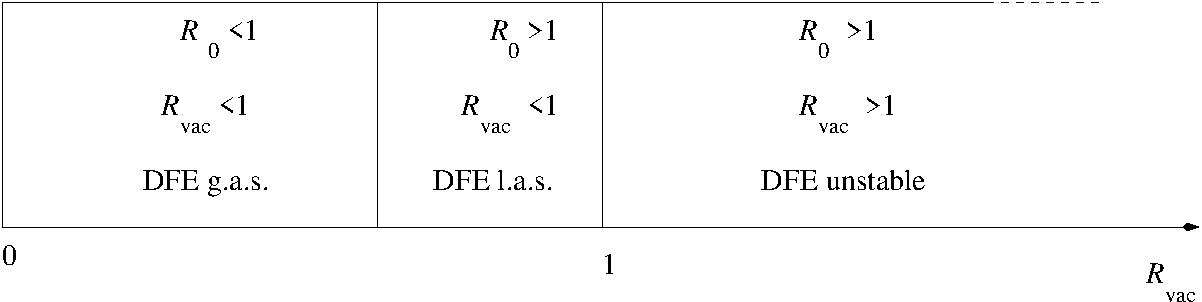
\includegraphics[width=0.95\textwidth]{FIGS/Rvac}
 \end{center}
\end{figure}
\end{frame}


%%%%%%%%%%%%%%%%%%%%%%%%%%
%%%%%%%%%%%%%%%%%%%%%%%%%%
\subsection{Case reducing to an ODE}
\newSubSectionSlide{FIGS-slides-admin/Gemini_Generated_Image_vqpscpvqpscpvqps.jpeg}

\begin{frame}\frametitle{Reduction of the system using specific $P(t)$ functions}
As before, two examples
\vfill
\begin{itemize}
\item The distribution of waning times is exponential, which leads to
 an ODE system. Treated briefly here, just so as to emphasize the
 presence of a so-called \emph{backward bifurcation}, a rather
 uncommon phenomenon in epidemiological models
\vfill
\item The waning time is a constant, which leads to a DDE model. We
 show that the backward bifurcation is also present
\end{itemize}
\end{frame}

\begin{frame}\frametitle{Case reducing to an ODE system}
Assume $P(v)=e^{-\theta v}$, $\theta>0$.
$V_0(t)=V_0(0)e^{-(d+\theta)t}e^{-\int_0^t\sigma\beta I(x)dx}$ from
(\ref{eq:V0}). Then (\ref{sys:SIVS_general_I}) and
(\ref{eq:Vprime_general}) give the ODE system
\begin{subequations}\label{ODEmodel}
\begin{align}
\frac{dI}{dt}&= \beta(1-I-(1-\sigma)V)I-(d+\gamma)I
\label{ODEmodelI}\\
\frac{dV}{dt}&= \phi(1-I-V)-\sigma\beta IV -(d+\theta)V+\alpha d
\label{ODEmodelV}
\end{align}
\end{subequations}
which with no newborn vaccination ($\alpha=0$) is the model studied in
Kribs-Zaletta \& Velasco-Hernandez, 2000 (extended to SIR with
vaccination: Arino,
McCluskey and van den Driessche).\\[0.2cm]

From Theorem~\ref{th:R0_gen_mod} the DFE always exists, with
\[
I_{DFE}=0,
S_{DFE}=\frac{\theta+d(1-\alpha)}{d+\theta+\phi},
V_{DFE}=\frac{\phi+\alpha d}{d+\theta+\phi}
\]
\end{frame}



\begin{frame}\frametitle{Backward bifurcation}
Assume that $\R_0>1$, then endemic equilibria (positive $I$
equilibria, denoted
by $I^\star$) can be obtained analytically from the quadratic equation
\[
\mathcal{P} (I)=AI^2+BI+C=0
\]
where
\begin{eqnarray*}
A&=& -\sigma\beta \\
B&=& \sigma(\beta-(d+\gamma))-(d+\theta+\sigma\phi)\\
C&=& (d+\gamma)(d+\theta+\phi)(\R_v-1)/\beta
\end{eqnarray*}
with
\[
\R_v=\R_0\frac{d+\theta+\sigma\phi-\alpha(1-\sigma)d}{d+\theta+\phi}
\]
from  (\ref{eq:generalRphi}).
\end{frame}

\begin{frame}
Backward bifurcation leading to two endemic
equilibria occurs for $\sigma>0$ if $ \mathcal{P}'(0)=B>0$,
$\mathcal{P}(0)=C<0$ and $B^2>4AC$ (we always have
$\mathcal{P}(1)<0$)
\vfill
\bbullet
On an $(\R_v,I)$ bifurcation diagram, this occurs for
$\R_c<\R_v<1$, where $\R_c$ is the value of $\R_v$ at
the saddle node bifurcation point where the two values of $I$ coincide,
\emph{i.e.}, $I=I_c=B/(-2A)$
\vfill
\bbullet
For $\R_v<\R_c$, there is no endemic equilibrium (EEP).
For $\R_v>1$, the constant term $C>0$, and there is a unique EEP
\vfill
\bbullet
In the case of forward bifurcation, $\R_c=1$; this is the case in
particular if the vaccine is totally effective ($\sigma=0$)
\end{frame}


\begin{frame}
By standard planar ODE arguments the following can be shown
\vfill
\begin{theorem}
For the ODE system (\ref{ODEmodel}) with $V(0)\geq 0$, $I(0)>0$, and
$\R_0>1$
\vskip0.3cm
(i) if $\R_v<\R_c$, then the disease dies out,
\vskip0.3cm
(ii) if $\R_c<\R_v<1$, then the EEP
with larger $I$ is l.a.s., and the EEP with smaller $I$ is unstable
\vskip0.3cm
(iii) if $\R_v>1$, then the unique EEP is globally
asymptotically stable in $\D-\{I=0\}$
\label{th:odecase}
\end{theorem}
\end{frame}

\begin{frame}
Pertussis:
\begin{itemize}
\item 3 week average disease duration ($\gamma=0.04762$)
\item Average lifetime 75 years ($d=3.6530E-05$)
\item Average number of adequate contacts per infective per day is
 estimated at 0.4 ($\beta=0.4$)
\item Most newborns are vaccinated in the first few months of life
 ($\alpha=0.9$)
\item  Vaccine is effective, $\sigma=0.1$ (90\% effective vaccine).
\item Pertussis vaccine begins to wane after about 3 years
 and the average waning time of the vaccine
 $1/\theta$ is assumed to be 5 years, giving $\theta=5.4794E-04$
\end{itemize}
\vfill
With these parameter values, there is backward
bifurcation for a range of $\phi$ values given by $0.0254\leq\phi\leq0.1506$
\end{frame}

\begin{frame}
\begin{minipage}{0.3\textwidth}
With the above parameter values, $\R_0=8.3936$ and $\R_v(\phi)=0.8807$ for
$\phi=0.1$, which is in the range of backward bifurcation since the
critical value $\R_c(\phi)=0.8669<\R_v(\phi)<1$
\end{minipage}
\begin{minipage}{0.68\textwidth}
   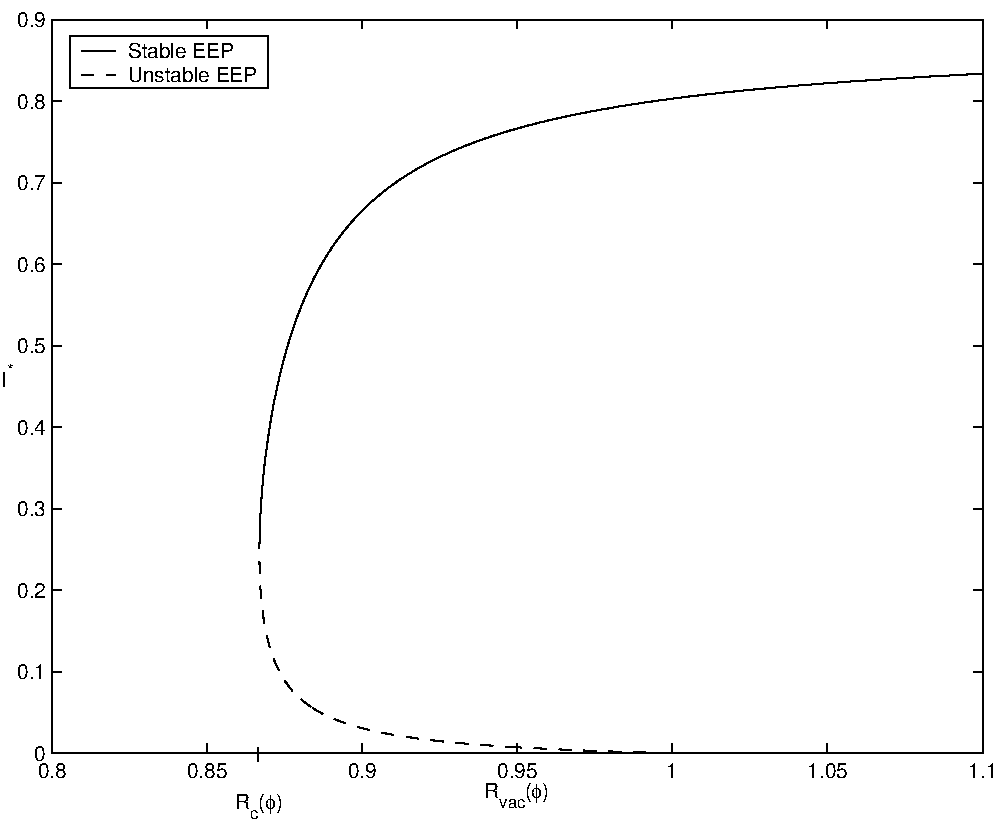
\includegraphics[width=\linewidth]{FIGS/SIV_ode_bif_phi}
\end{minipage}
\end{frame}

%%%%%%%%%%%%%%%%%%%%%%%%%%
%%%%%%%%%%%%%%%%%%%%%%%%%%
\subsection{Case reducing to a DDE}
\newSubSectionSlide{FIGS-slides-admin/Gemini_Generated_Image_vqpscpvqpscpvqps.jpeg}

\begin{frame}\frametitle{Step function case: a delay integral model}
Suppose that
\[ 
P(v)=
\left\{
\begin{array}{l}
1\textrm{ if }v\in[0,\omega] \\
0\textrm{ otherwise} 
\end{array}
\right.
\]
Since $V_0(t)=0$ for $t>\omega$, with $S=1-I-V$ the
integral equation \eqref{sys:SIVS_general_V} becomes, for $t>\omega$
\begin{equation}
  V(t)=\int_{t-\omega}^t(\phi (1-I(u)-V(u))+\alpha d)e^{-d(t-u)}
  e^{-\sigma\beta\int_u^tI(x)dx}du
  \label{eq:VoftStepCase}
\end{equation}
\end{frame}

\begin{frame}
Differentiating \eqref{eq:VoftStepCase} (see equation
\eqref{eq:Vprime_general}) gives the model as the two
dimensional system, for $t>\omega$
\begin{subequations}\label{sys:SIVS_DDE}
\begin{align}
  \frac{d}{dt}I(t) &= 
  \beta(1-I(t)-(1-\sigma)V(t))I(t)-(d+\gamma)I(t) \label{sys:SIVS_DDE_dS} \\
  \frac{d}{dt}V(t) &=
  \phi(1-I(t)-V(t)) \label{sys:SIVS_DDE_dV}\\
  &\qquad-\phi(1-I(t-\omega)-V(t-\omega))e^{-d\omega}
  e^{-\sigma\beta\int_{t-\omega}^t I(x)dx} \nonumber \\
  &\qquad -\sigma\beta IV-dV
  +\alpha d\left(1-e^{-d\omega}e^{-\sigma\beta\int_{t-\omega}^t I(x)dx}
  \right) \nonumber
\end{align}
\end{subequations}
Hereafter, shift time by $\omega$ so that these equations hold for $t>0$
\end{frame}


\begin{frame}
The well posedness of the problem follows from
Theorem~\ref{th:invariance_gen_model} and from the fact that solutions
of (\ref{sys:SIVS_general}) exist and are unique.
For a constant waning period, the basic reproduction number from
(\ref{eq:generalRphi}) is
\begin{equation}
 \R_v = \R_0
 \frac{d+(\sigma\phi-\alpha(1-\sigma)d)
 (1-e^{-d\omega})}{d+\phi(1-e^{-d\omega})}
 \label{eq:Rphi}
\end{equation}


With $I_{DF}=0$, from Theorem~\ref{th:R0_gen_mod}
\begin{equation}
 V_{DF}=\frac{(\phi+\alpha d)(1-e^{-d\omega})}{d+\phi(1-e^{-d\omega})}
,\,\,
S_{DF}=\frac{d-\alpha d(1-e^{-d\omega})}{d+\phi(1-e^{-d\omega})}
 \label{eq:DFE_V}
\end{equation}
\end{frame}

\begin{frame}\frametitle{Finding the EEP's}
From nullclines, there exists one (or more) endemic equilbria
(EEP) iff there exists $0<I^\star\leq 1$ such that
\begin{equation}
 V^\star=f(I^\star)=g(I^\star)
 \label{eq:f_egal_g}
\end{equation}
where
\begin{equation}
 f(I)=\frac{1-1/\R_0-I}{1-\sigma}
 \label{eq:f(I)}
\end{equation}
for $\sigma<1$, and
\begin{equation}
 g(I)=\frac{(\phi(1-I)+\alpha d)(1-e^{-d\omega-\sigma\beta\omega I})}
 {\phi(1-e^{-d\omega-\sigma\beta\omega I})+d+\sigma\beta I}
 \label{eq:g(I)}
\end{equation}
\end{frame}


%%%%%%%%%%%%%%%%%%%
%%%%%%%%%%%%%%%%%%%
\begin{frame}\frametitle{Visualising and locating the bifurcation}
From the nullcline equations, an EEP exists iff there exists an
$I^\star\in(0,1]$ such that equations (\ref{eq:f_egal_g})-(\ref{eq:g(I)})
hold.
So we study the zeros of
\[
H(I)=\frac{1-1/\R_0-I}{1-\sigma} -
\frac{(\phi(1-I)+\alpha d)(1-e^{-d\omega-\sigma\beta\omega I})}
{\phi(1-e^{-d\omega-\sigma\beta\omega I})+d+\sigma\beta I}
\]
To state the problem in a formal way, let
$\mathcal{A}=\{\alpha,\beta,\gamma,\omega,\phi,\sigma\}$ be the set of
parameters of interest, and denote
\begin{equation}
H(I,\mathcal{A})=
f(I)-g(I)
\label{eq:H}
\end{equation}
to show the dependence on these parameters.
\end{frame}

\begin{frame}
We proceed as follows.
\begin{enumerate}
\item Choose a parameter $a_i\in\mathcal{A}$.
\item Fix all other $a_j$'s ($j\neq i$).
\item Choose $a_{i,min}$, $a_{i,max}$ and
 $\Delta a_i$ for $a_i$.
\item For all
  $a_{i,k}=a_{i,min}+k\Delta a_i$ ($k$
  such that $a_{i,k}\leq a_{i,max}$), compute
  $I^\star$ such that $H(I^\star,a_{i,k})=0$. \label{point1}
\end{enumerate}
Step~\ref{point1} is carried out using the {\sc MatLab} {\tt fzero}
function.

Further precision can be gained by showing that
\[
H(0)=\frac{\R_v-1}{(1-\sigma)\R_0}
\]
and that, for $\sigma<1$
\[
H(1)=-\frac{1}{(1-\sigma)\R_0}-\frac{\alpha
d(1-e^{-d\omega-\sigma\beta\omega})}{\phi(1
-e^{-d\omega-\sigma\beta\omega})+d+\sigma\beta}<0
\]
\end{frame}

\begin{frame}
Define $\R_c$ as previously. For $\R_0>1$ and
$\R_v<1$, there are several possibilities.
\begin{itemize}
\item If $\R_v<\R_c$, then there is no EEP. $H(0)$ and $H(1)$
 are strictly negative, and numerical simulations seem to indicate
 that $H$ has no roots in $(0,1]$ (\emph{i.e.}, that $H<0$ on this
 interval).
\item If $\R_c<\R_v<1$, then there are endemic equilibria.
 Here, since $H(0)$
 and $H(1)$ are strictly negative, the only possibility is thus to
 have an even number of zeros of $H$. Numerical simulations appear to
 indicate that the number of endemic equilibria is 2.
\end{itemize}
In between these two situations $\R_v=\R_c$ and there is
one endemic equilibrium $I^\star$. Using the same procedure as for the
visualisation of the bifurcation, it is possible to compute
$\R_c$ by finding the value $I^\star$ such that
$H(I^\star,\mathcal{A})=0$ and $H'(I^\star,\mathcal{A})=0$, for a given
parameter $a_i\in\mathcal{A}$.

If $\R_v>1$ then $H(0)>0$ and so there is an odd number of endemic
equilibria. Numerical simulations indicate that there is a unique
EEP.
\end{frame}

\begin{frame}\frametitle{Numerical bifurcation analysis}
Same parameter values as in ODE case, except that the
constant waning time
(the delay) $\omega$ has to be substituted for $\theta$. We take
$\omega=1825$, \emph{i.e.}, corresponding to a 5 years waning time
\vfill
These parameters give $\R_0=8.3936$ and $\R_v(\phi)=0.8819$, which
is in the range of the backward bifurcation since (using the above
method) $\R_c(\phi)=0.8675$
\vfill
The bifurcation diagram is very like that depicted in
earlier for the ODE. Numerical simulations of the DDE model
(using {\tt dde23}) indicate that there are no additional
bifurcations; solutions either go to the DFE or to the (larger) EEP
\end{frame}


\begin{frame}
\begin{center}
   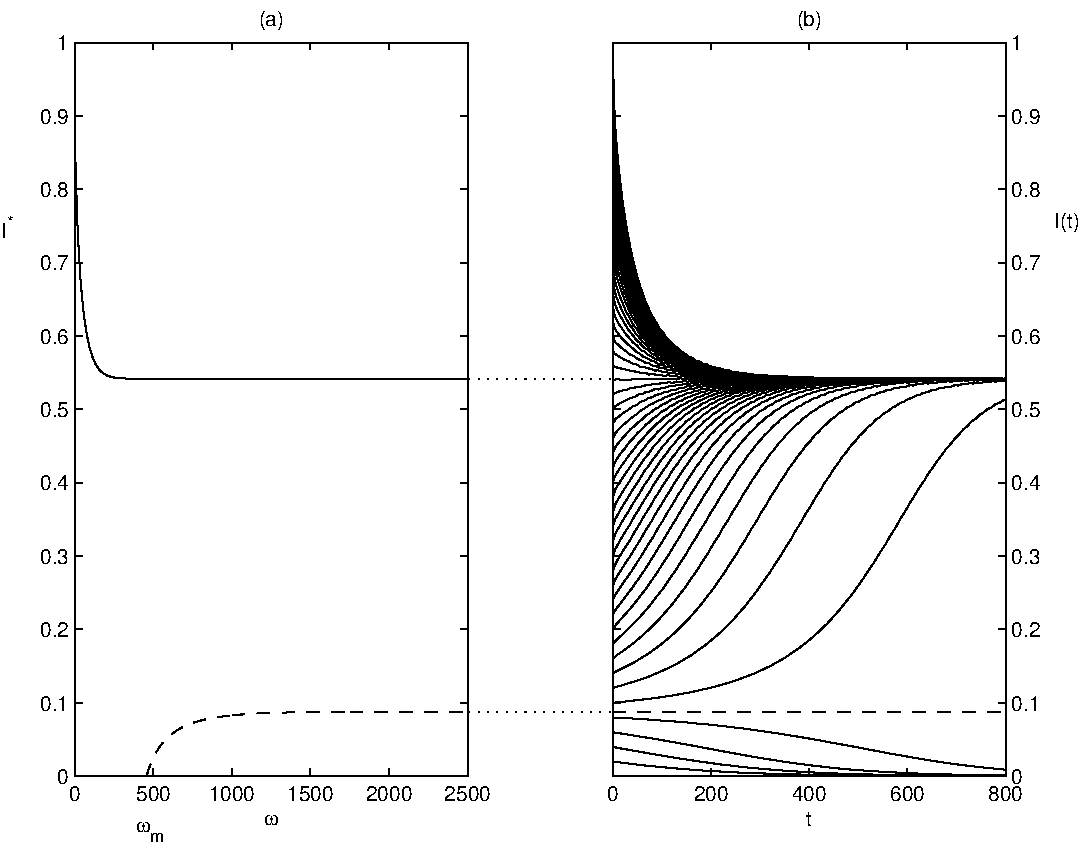
\includegraphics[width=0.6\textwidth]{FIGS/bif_and_time}
\end{center}
(a) Values of $I^\star$ as a function of $\omega$ by solving $H(I,\mathcal{A})=0$ with $a_i=\omega$. (b) Value of $I(t)$ versus time, obtained by numerical integration of system \eqref{sys:SIVS_DDE} with initial data $I(t)=c$, for $t\in[-\omega,0]$, $\omega=1825$, $c$ varying from 0 to 1 by steps of 0.02
\end{frame}


%%%%%%%%%%%%%%%%
%%%%%%%%%%%%%%%%
%%%%%%%%%%%%%%%%
%%%%%%%%%%%%%%%%
\section{Age of infection}
\newSectionSlide{FIGS-slides-admin/Gemini_Generated_Image_vqpscpvqpscpvqps.jpeg}

\begin{frame}\frametitle{Age of infection}
We have seen that infinite dimensionality could result from a detailed description (or an unspecified one) of the sojourn time in compartments
\vfill
Originally, age of infection was introduced to account for differences in infectivity depending on the time since an individual became infected
\vfill
For instance, it is known that infectiousness of HIV positive patients vary as a function of time since infection
\end{frame}

%%%%%%%%%%%%%%%%
%%%%%%%%%%%%%%%%
%%%%%%%%%%%%%%%%
\subsection{Age of vaccination}
% The section page
\newSubSectionSlide{FIGS-slides-admin/Gemini_Generated_Image_5yvymh5yvymh5yvy.jpeg}


\begin{frame}\frametitle{Age of vaccination}
We used age of vaccination to find the initial condition of \eqref{sys:SIVS_general}
\vfill
Here we take a closer look at this type of model
\end{frame}



\maxFrameImage{FIGS/BowmanArinoMoghadas-2011-cover.png}

\begin{frame}{How to model time between vaccine doses}
\begin{subequations}
\begin{align}
S\pprime &= -fS-V_1(t,0) \\
A\pprime &= \left(
(1-p)S+(1-p_1)\delta_1\tilde V_1+(1-p_2)\delta_2 V_2
\right)f-\mu_AA \\
I\pprime &= (pS+p_1\delta_1\tilde V_1+p_2\delta_2 V_2)f-\mu I \\
V_2\pprime &= V_1(t,a^\star)-\delta_2fV_2(t)
\end{align}
\begin{equation}\label{eq:V1_age_time}
\left(
\frac{\partial}{\partial t}+\frac{\partial}{\partial a}
\right) V_1(t,a) = -\delta_1fV_1(t,a),\quad 0\leq a\leq a^\star
\end{equation}
and boundary condition
\begin{equation}
V_1(t,0) = \begin{cases}
\gamma S_0\left(\frac{S(t)}{S(t)+A(t)}\right) & \text{if } T\leq t\leq T_e \text{ and }S>0 \\
0 & \text{otherwise}
\end{cases}
\end{equation}
\end{subequations}
where $f=\beta(\delta_AA+I)$ and $\tilde V_1(t)=\int_0^{a^\star}V_1(t,a)da$
\end{frame}

\begin{frame}{Simplifying a bit}
Integrate \eqref{eq:V1_age_time} using characteristics along lines $a=s$ and $t=T+s$, with $s$ as a new variable
\begin{equation}\label{eq:V1_age_time_integrated}
V_1(t,a)=V_1(t-a,0)\exp\left(\int_{t-a}^t -\delta_1f(\xi)\ d\xi\right)
\end{equation}
Define
\[
\zeta(t)=\int_0^t\delta_1f(\xi)d\xi
\]
and substitute into \eqref{eq:V1_age_time_integrated}, giving
\[
V_1(t,a)=V_1(t-a,0)\exp\left(\zeta(t-a)\zeta(t)\right)
\]
So the distributed delay is now discrete
\end{frame}

\begin{frame}{Simplifying a bit more}
Let
\[
\nu(t)=\int_0^t V_1(s,0)e^{\zeta(s)}ds
\]
Then the total number of individuals having been vaccinated with a single dose is
\[
\tilde V_1(t)=e^{-\zeta(t)}
\left(
\nu(t)-\nu(t-a^\star)
\right)
\]
\begin{subequations}
\begin{align}
S\pprime &= -fS-V_1(t,0) \\
A\pprime &= \left(
(1-p)S+(1-p_1)\delta_1\tilde V_1+(1-p_2)\delta_2 V_2
\right)f-\mu_AA \\
I\pprime &= (pS+p_1\delta_1\tilde V_1+p_2\delta_2 V_2)f-\mu I \\
V_2\pprime &= V_1(t-a^\star,0)e^{\zeta(t-a^\star)}-\delta_2fV_2(t) \\
\zeta\pprime &= \delta_1f \\
\nu\pprime &= V_1(t,0)e^{\zeta(t)}
\end{align}
\end{subequations}
\end{frame}


%%%%%%%%%%%%%%%%
%%%%%%%%%%%%%%%%
%%%%%%%%%%%%%%%%
%%%%%%%%%%%%%%%%
\section{Structuration in age}
\newSectionSlide{FIGS-slides-admin/Gemini_Generated_Image_sw1w5bsw1w5bsw1w.jpeg}

% \begin{frame} 
% \begin{tikzpicture}[remember picture, overlay]
%     \node[anchor=center, 
%     inner sep=0pt,
%     opacity=0.95] (image) at (current page.center) 
%     {\includegraphics[height=\paperheight, keepaspectratio]{FIGS/Pierre-Magal.jpg}};
%    \node[anchor=north, 
%    align=center, 
%    text=black, 
%    font=\Large] at (image.north) 
%    {Pierre Magal\\(1967-10-24 -- 2024-02-20)}; 
% \end{tikzpicture}
% \end{frame}
% 



\begin{frame}\frametitle{Age structure}
Taking into account age can be important in some cases
\vfill
\begin{itemize}
\item Demographic characteristics vary with age
\item Interactions are in general more frequent between people of a similar age. They are also more frequent in younger individuals
\item Some diseases attack preferentially younger individuals
\item The immunity of individuals changes with age, so for instance, older people may be more susceptible to some diseases than younger people
\end{itemize}
\vfill
This is based on courses given by Jia Li during a Banff summer school in 2004 \nocite{li2008continuous}
\end{frame}

\maxFrameImage{FIGS/BrauerPvdDWu-book.png}
\nocite{brauer2008mathematical}

\begin{frame}{Note on age}
\defword{Chronological age}, as a structuring variable, is ``easier'' than other structuring variables
\vfill
Indeed, if $a$ is (chronological) age, then
\[
\frac{d}{dt}a = 1
\]
\end{frame}


\begin{frame}\frametitle{Formulation of an SIR model}
Let $a$ be the age. Assume that natural death and recovery occur at the rates $\mu$ and $\gamma$, respectively, both dependent on $a$
\vfill
When an individual is sick, they are subject to disease-induced death at the rate $\delta(a)$
\vfill
Governing equations are
\footnotesize
\begin{subequations}\label{sys:SIR_age_structure}
\begin{align}
(\partial_t+\partial_a)S(t,a) &=
\Lambda(a)-(\mu(a)+\lambda(t,a))S(t,a)
\label{sys:SIR_age_structure_S} \\
(\partial_t+\partial_a)I(t,a) &=
-(\mu(a)+\gamma(a)+\delta(a))I(t,a)+\lambda(t,a)S(t,a)
\label{sys:SIR_age_structure_I} \\
(\partial_t+\partial_a)R(t,a) &=
\gamma(a)I(t,a)
\label{sys:SIR_age_structure_R}
\end{align}
\end{subequations}
\end{frame}

\begin{frame}
Boundary conditions are
\addtocounter{equation}{-1}\
\begin{subequations}
\setcounter{equation}{3}
\begin{align}
S(t,a_0)&=B \label{sys:SIR_age_structure_BCS} \\
I(t,a_0)&=0 \label{sys:SIR_age_structure_BCI} \\
R(t,a_0)&=0 \label{sys:SIR_age_structure_BCR}
\end{align}
while initial conditions take the form
\begin{align}
S(0,a)&=\Phi(a) \label{sys:SIR_age_structure_ICS} \\
I(0,a)&=\Psi(a) \label{sys:SIR_age_structure_ICI} \\
R(0,a)&=0 \label{sys:SIR_age_structure_ICR}
\end{align}
\end{subequations}
\end{frame}

\begin{frame}{Force of infection}
Transmission $\lambda(t,a)$ of the disease takes the form
\[
\lambda(t,a)=r(a)\int_{a_0}^\infty \beta(a,s)\rho(a,s)
\frac{I(t,s)}{N(t,s)}ds
\]
where 
\begin{itemize}
\item $r(a)$ is the number of contacts by individuals of age $a$ per unit time
\item $\beta(a,s)$ is the probability of disease transmission to a susceptible of age $a$ by an infectious of age $s$
\item $\rho(a,s)$ is the meeting rate between people of age $a$ and people of age $s$
\item $N(t,a)=S(t,a)+I(t,a)+R(t,a)$ is the distribution of total population
\end{itemize}
\end{frame}


\begin{frame}
To simplify, assume that $\beta(a,s)$ is separable
\[
\beta(a,s)=f(a)g(s)
\]
where $f(a)$ is the susceptibility of individuals aged $a$ and $g(s)$ is the force of infection of individuals aged $s$
\vfill
Then
\begin{equation}\label{eq:beta_age_dep}
\lambda(t,a)=r(a)f(a)\int_{a_0}^\infty g(s)\rho(a,s)
\frac{I(t,s)}{N(t,s)}ds
\end{equation}
\end{frame}

%%%%%%%%%%%%%%%%
%%%%%%%%%%%%%%%%
\begin{frame}\frametitle{Analysis of the SIR model}
We seek the DFE by setting $I=0$
\vfill
We find $(S,I,R)=(S^0(a),0,0)$ with
\[
S^0(a)=Be^{-M(a)} +e^{-M(a)}\int_{a_0}^a e^{M(x)}\Lambda(x)dx
\]
where
\[
M(a)=\int_{a_0}^a \mu(s)ds
\]
\end{frame}


\begin{frame}
Consider the perturbed solution $u(t,a)=S(t,a)-S^0(a)$. Assume that the meeting rate $\rho$ is also separable,
\[
\rho(a,s)=p_1(a)p_2(s)
\]
Then
\[
\tilde\lambda(t,a):=r(a)f(a)p_1(a)\int_{a_0}^\infty
\frac{g(s)p_2(s)}{S^0(s)}I(t,s) ds \simeq \lambda(t,a)
\]
and we obtain the linearisation
\begin{align*}
(\partial_t+\partial_a)u&=-\mu(a)u-\tilde\lambda(t,a)S^0(a) \\
(\partial_t+\partial_a)I&=-(\mu(a)+\gamma(a)+\delta(a))I
+\tilde\lambda(t,a)S^0(a) \\
(\partial_t+\partial_a)R&=\gamma(a)I
\end{align*}
\end{frame}


\begin{frame}
Let
\[
u(t,a)=\tilde u(a)e^{c(t-a)}\quad\quad I(t,a)=\tilde I(a)e^{c(t-a)}
\]
and denote
\[
b(a)=S^0(a)r(a)f(a)p_1(a)\quad\quad W=\int_{a_0}^\infty
\frac{g(s)p_2(s)}{S^0(s)}e^{-cs}\tilde I(s)ds
\]
\end{frame}


\begin{frame}
Then
\begin{align*}
\frac{d\tilde u(a)}{da} &= -\mu(a)\tilde u(a)-b(a)e^{ca}W \\
\frac{d\tilde I(a)}{da} &= -(\mu(a)+\gamma(a))\tilde I(a)+b(a)e^{ca}W
\end{align*}
\[
\tilde I(a)=We^{-M(a)-\Gamma(a)}\int_{a_0}^\infty
e^{M(s)+\Gamma(s)}b(s)e^{cs}ds
\]
where $\Gamma(a)=\int_{a_0}^a\gamma(s)ds$
\vfill
Therefore
\[
W=W\int_{a_0}^\infty \frac{g(s)p_2(s)}{S^0(s)}e^{-M(s)-\Gamma(s)}
\int_{a_0}^s e^{M(v)+\Gamma(v)}b(v)e^{-c(s-v)}dvds
\]
\end{frame}

\begin{frame}
Let then
\[
H(c):=\int_{a_0}^\infty \frac{g(s)p_2(s)}{S^0(s)}e^{-M(s)-\Gamma(s)}
\int_{a_0}^s e^{M(v)+\Gamma(v)}b(v)e^{-c(s-v)}dvds
\]
\vfill
We seek roots of the characteristic equation $H(c)=1$
\vfill
We have
{\footnotesize
\[
\frac{dH(c)}{dc}=-\int_{a_0}^\infty
\frac{g(s)p_2(s)}{S^0(s)}e^{-M(s)-\Gamma(s)}
\int_{a_0}^s (s-v)e^{M(v)+\Gamma(v)}b(v)e^{-c(s-v)}dvds<0
\]}
implying that $H(c)$ is a decreasing function
\end{frame}


\begin{frame}
\bbullet 
Let $c^\star$ be a real solution to $H(c)=1$. If $H(0)>1$, then $c>0$, whereas if $H(0)<1$, $c<0$
\vfill
\bbullet
Suppose that $c^\star=\alpha+i\beta$ is a complex root of $H(c)=1$. Then
{\footnotesize
\[
\Re H(c)=
\int_{a_0}^\infty \frac{g(s)p_2(s)}{S^0(s)}e^{-M(s)-\Gamma(s)}
\int_{a_0}^s e^{M(v)+\Gamma(v)}b(v)e^{-\alpha(s-v)}\cos\beta(s-v)dvds
\]}
As a consequence, $H(0)<1$ $\implies$ $\alpha<0$
\vfill
So $H(0)=1$ is a threshold and we take $\R_0=H(0)$
\end{frame}


%%%%%%%%%%%%%%%%
%%%%%%%%%%%%%%%%
\begin{frame}{Analysis using semigroups: SIA model}
To illustrate the use of the semigroup method in this context, we consider an SIA model describing the evolution of HIV/AIDS
\vfill
The model is almost equivalent to \eqref{sys:SIR_age_structure}, with a few differences
\vfill
The $I$ compartment contains inviduals bearing HIV, but not yet in the AIDS stage
\vfill
The rate $\gamma(a)$ represents the progression towards the AIDS stage
\vfill
The AIDS stage is represented by compartment $A$, where individuals are subject 
to a specific mortality rate
\end{frame}

\begin{frame}
\begin{subequations}\label{sys:SIA_age_structure}
\begin{align}
(\partial_t+\partial_a)S(t,a) &=
\Lambda(a)-(d(a)+\lambda(t,a))S(t,a)
\label{sys:SIA_age_structure_S} \\
(\partial_t+\partial_a)I(t,a) &=
-(d(a)+\gamma(a))I(t,a)+\lambda(t,a)S(t,a)
\label{sys:SIA_age_structure_I} \\
(\partial_t+\partial_a)A(t,a) &=
\gamma(a)A(t,a)-(d(a)+\delta(a))A(t,a)
\label{sys:SIA_age_structure_R}
\end{align}
\vfill
Assume
\begin{equation}\label{sys:SIA_age_structure_force_infection}
\lambda(t,a)=h(a)\int_{a_0}^\infty \rho(a,a')
\frac{I(t,a')}{T(t,a')}da'
\end{equation}
\end{subequations}
where $T(t,a')=S(t,a')+I(t,a')$
\end{frame}

\begin{frame}
An individual in AIDS stage no longer has contacts. Therefore the dynamics of $S$ and $I$ do not depend on the dynamics of $A$, and we consider the system consisting of the first two variables
\vfill
Let $\omega$ be the maximum age. The system in proportions takes the form
\[
x:=\frac ST\quad\quad y:=\frac IT
\]
\vfill
As we are only considering $S$ and $I$, we have $x+y=1$ and the system reads
\begin{subequations}\label{sys:SIA_age_struct}
\begin{align}
(\partial_t+\partial_a)y(t,a)&=(1-y)(-\gamma(a)y+\lambda(t,a)) \\
\lambda(t,a)&=h(a)\int_0^\omega p(a,a')y(t,a')da'
\end{align}
\end{subequations}
\end{frame}



\begin{frame}
Let $X=\{f\in L^1(0,\omega)\}$. Define
\[
(Af)(a):=-\frac{d}{da}f(a),\quad f\in D(A)
\]
with $D(a)=\{f\in X,\; f\text{ is absolutely continuous, }f(0)=0\}$,
and
\[
F(f)(a)\equiv (1-f(a))\left(
-\gamma(a)f(a)+h(a)\int_0^\omega p(a,a')f(a')da'\right)
\]
an operator from $X\to X$
\vfill
Let $\Omega=\{f\in X,\; 0\leq f\leq 1\textrm{ a.e.}\}$. Then
\eqref{sys:SIA_age_struct} takes the form
\begin{align*}
\frac{dy}{dt}&= Ay+F(y) \\
y(0)&= y_0\in\Omega
\end{align*}
\end{frame}



\begin{frame}
Let
\[
(\mathcal{B}f)(a)=-\frac{df(a)}{da}-\gamma(a)f(a)
\quad\quad
(\mathcal{P}f)(a)=h(a)\int_0^\omega p(a,a')f(a')da'
\]
\vfill
We have
\[
(\partial_t+\partial_a)y=-\gamma(a)y+h(a)\int_0^\omega
\rho(a,a')y(t,a')da' \Leftrightarrow
\frac{dy}{dt}=(\mathcal{B}+\mathcal{P})y
\]
\vfill
$\mathcal{B}+\mathcal{P}$ generates a $C_0$-semigroup $T(t)$,
$t\geq 0$, which is eventually uniformly continuous
%Les bornes
%de croissance de $T$ sont donn\'e par les bornes spectrales de
%$\mathcal{B}+\mathcal{P}$.
\end{frame}


\begin{frame}
The  resolvant of $\mathcal{B}+\mathcal{P}$ is
\[
R(\lambda;\mathcal{B}+\mathcal{P})=(S_\lambda-I)^{-1}G
\]
with
\[
(Gf)(a)=\int_0^a
e^{-\lambda(a-\sigma)}\frac{\Gamma(a)}{\Gamma(\sigma)}
f(\sigma)d\sigma
\]
\[
(S_\lambda f)(a)=\int_0^\omega\int_0^a
e^{-\lambda(a-\sigma)}\frac{\Gamma(a)}{\Gamma(\sigma)}
\rho(\sigma,\xi)d\sigma f(\xi)d\xi
\]
where we denoted
\[
\Gamma(a)=\exp\left(-\int_0^a \gamma(a')da'\right)
\]
\end{frame}


\begin{frame}\frametitle{$\R_0$}
$\R_0$ is the spectral radius of the operator
\[
(Sf)(a)=\int_0^\omega\int_0^a \frac{\Gamma(a)}{\Gamma(\sigma)}
h(\sigma)p(\sigma,\xi)d\sigma f(\xi)d\xi
\]
\end{frame}


\begin{frame}\frametitle{Pair formation}
$\rho(t,a,a')$ proportion of partners of an individual aged $a$ who are aged $a'$
\vfill
$r(t,a)$ mean number of partners of an individual aged $a$
\vfill
$T(t,a)$ total number of individuals aged $a$
\vfill
The following conditions must hold
\begin{itemize}
\item $0\leq\rho\leq 1$
\item $\int_0^\infty \rho(t,a,a')da'=1$
\item $\rho(t,a,a')r(t,a)T(t,a)=\rho(t,a',a)r(t,a')T(t,a')$
\item $r(t,a)T(t,a)r(t,a')T(t,a')=0\Rightarrow \rho(t,a,a')=0$
\end{itemize}
\end{frame}

\begin{knitrout}
\definecolor{shadecolor}{rgb}{0.969, 0.969, 0.969}\color{fgcolor}\begin{kframe}
\begin{alltt}
\hlcom{# From https://stackoverflow.com/questions/36868287/purl-within-knit-duplicate-label-error}
\hldef{rmd_chunks_to_r_temp} \hlkwb{<-} \hlkwa{function}\hldef{(}\hlkwc{file}\hldef{)\{}
  \hldef{callr}\hlopt{::}\hlkwd{r}\hldef{(}\hlkwa{function}\hldef{(}\hlkwc{file}\hldef{,} \hlkwc{temp}\hldef{)\{}
    \hldef{out_file} \hlkwb{=} \hlkwd{sprintf}\hldef{(}\hlsng{"../CODE/%s"}\hldef{,} \hlkwd{gsub}\hldef{(}\hlsng{".Rnw"}\hldef{,} \hlsng{".R"}\hldef{, file))}
    \hldef{knitr}\hlopt{::}\hlkwd{purl}\hldef{(file,} \hlkwc{output} \hldef{= out_file,} \hlkwc{documentation} \hldef{=} \hlnum{1}\hldef{)}
  \hldef{\},} \hlkwc{args} \hldef{=} \hlkwd{list}\hldef{(file))}
\hldef{\}}
\hlkwd{rmd_chunks_to_r_temp}\hldef{(}\hlsng{"course-02-metapopulations-and-advanced-models.Rnw"}\hldef{)}
\end{alltt}


{\ttfamily\noindent\bfseries\color{errorcolor}{\#\# Error: ! in callr subprocess.\\\#\# Caused by error in `file(con, "{}r"{})`:\\\#\# ! cannot open the connection}}\end{kframe}
\end{knitrout}

\begin{frame}[allowframebreaks]{Bibliography}
\bibliographystyle{apalike}
\bibliography{local-bibliography}
\end{frame}


\end{document}
